\chapter{Część praktyczna}
Cykl życia standardowej strony internetowej może przedstawić od następujących kroków przedstawionych na rysunku \ref{fig:rysunek_7}

\begin{figure}[htbp]
    \centering
    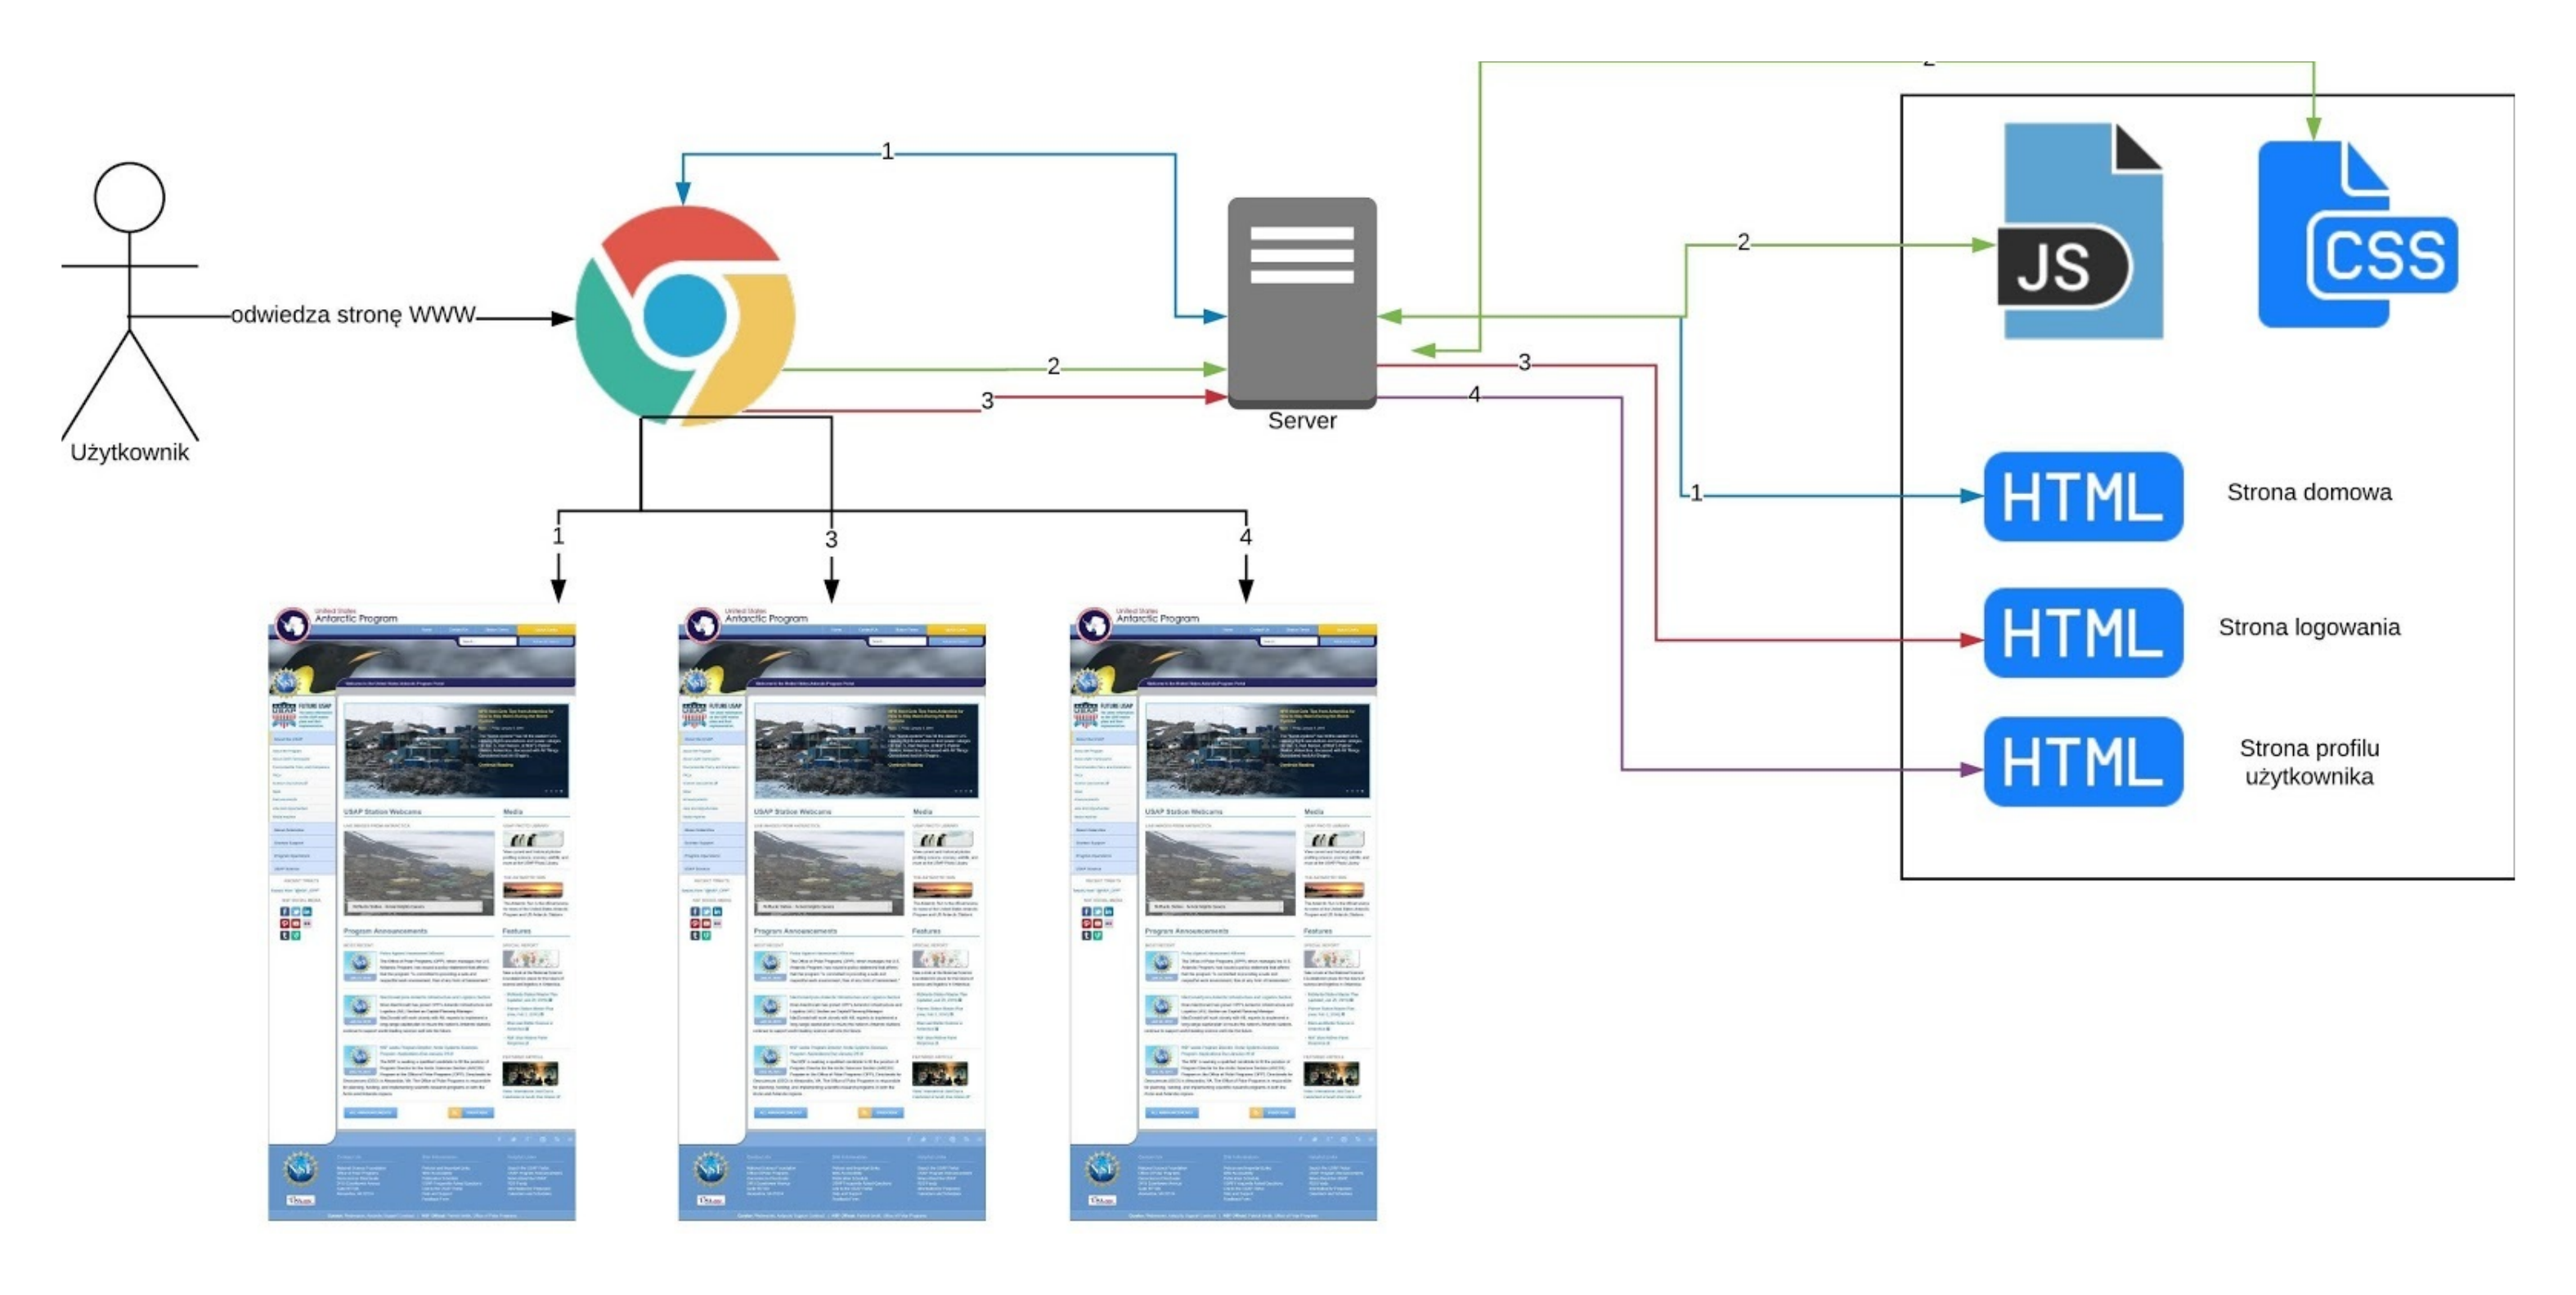
\includegraphics[width=14cm]{rysunek_7.png}
    \caption{Ilustracja przedstawiająca cykl życia statycznej strony internetowej}
    \label{fig:rysunek_7}
\end{figure}

\begin{itemize}
	\item Użytkownik otwiera przeglądarkę i odwiedza stronę WWW;
    \item Przeglądarka wysyła zapytanie do serwera z żądaniem zasobów;
    \item Serwer odsyła plik HTML w którym znajdują się odnośniki do plików JavaScript oraz CSS;
    \item Przeglądarka pobiera pliki JavaScript oraz CSS;
    \item Przeglądarka renderuje stronę dla użytkownika;
    \item Użytkownik klika w odnośnik do kolejnej strony ( w przykładzie strona logowania);
    \item Przeglądarka pobiera cały nowy plik HTML;
    \item Przeglądarka renderuje nową stronę od nowa;
    \item Przeglądarka ponownie pobiera dodatkowe pliki JavaScript oraz CSS (zakładamy, że przeglądarka nie przechowuje plików w pamięci podręcznej);
    \item Przeglądarka renderuje stronę od nowa.
\end{itemize}

Jak zostało przedstawione, cały proces odwiedzenia dwóch stron w tej samej domenie wymaga każdorazowego przeładowania strony oraz pobrania tych samych danych.
Proces ten wymaga ciągłego pobierania plików HTML, pobierania plików dodatkowych co obciąża procesor, pamięć łącze oraz sam serwer.

Dla porównania, przedstawiona poniżej ilustracja pokazuje cykl działania aplikacji SPA (rysunek \ref{fig:rysunek_8})

\begin{figure}[htbp]
    \centering
    \advance\leftskip-3.5cm
    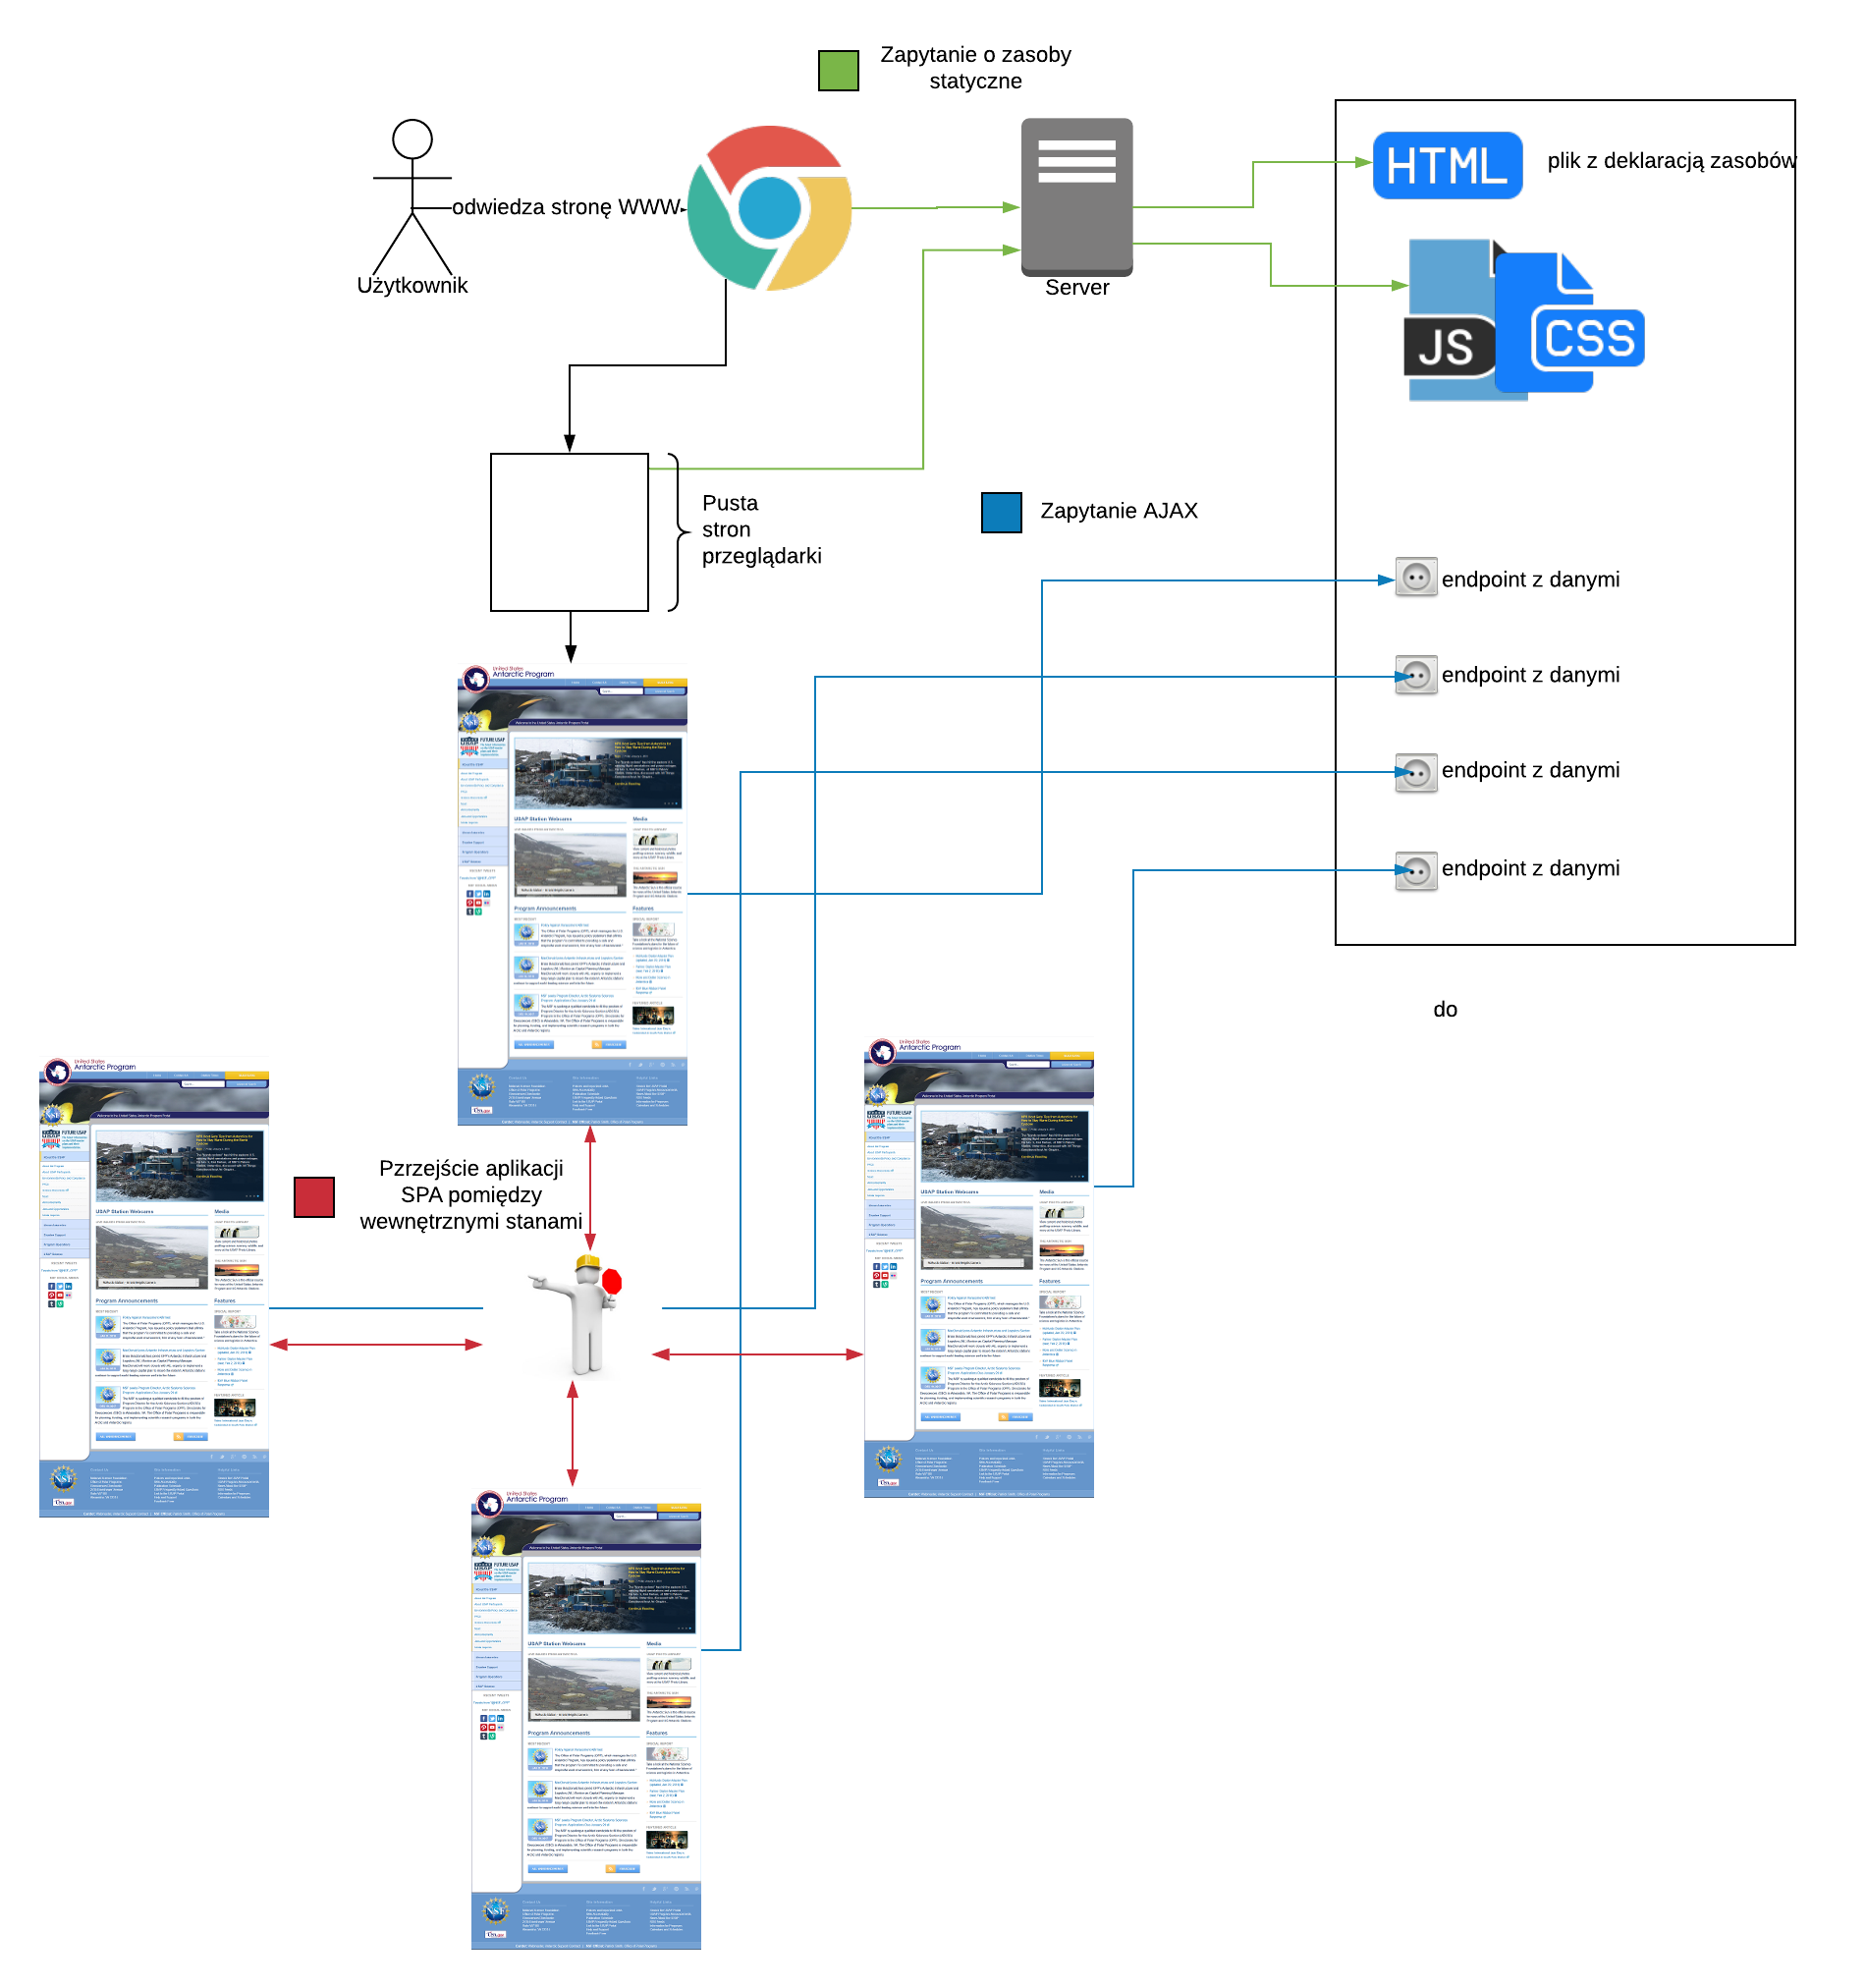
\includegraphics[width=22cm]{rysunek_8.png}
    \caption{Ilustracja przedstawiająca cykl działania aplikacji SPA}
    \label{fig:rysunek_8}
\end{figure}

\begin{itemize}
    \item Użytkownik odwiedza tę samą stronę;
    \item Przeglądarka pobiera plik HTML z definicją potrzebnych zasobów. Zazwyczaj sekcja body pliku jest pusta;
    \item Przeglądarka pobiera dodatkowe pliki JavaScript oraz CSS;
    \item Często pliki te są zoptymalizowane poprzez kompresję i sklejone w jeden plik tak, aby wykonać tylko jedno zapytanie zamiast dwóch;
    \item Pliki JavaScript, generują treść strony HTML;
    \item Przeglądarka może ( ale nie musi ) wykonać dodatkowe zapytanie o dane do jednego z endpointów serwera;
    \item Użytkownik klika na odnośnik do kolejnej strony. Przeglądarka nie pobiera już dodatkowego pliku HTML, jako, że aplikacja jest dynamiczna. Skrypt JavaScript może, ale nie musi pobrać dodatkowych informacji z serwera.
\end{itemize}

Jak zostało przedstawione, wykonano znacznie mniej zapytań do serwera. Dodatkowe zapytania które skrypt może wykonać w celu pobrania danych zazwyczaj są znacznie mniejsze od pełnego pliku HTML z wybraną treścią.
Dodatkowo, przeglądarka nie przeładowuje strony przy każdej zmianie podstrony, co także odciąża procesor jak i łącze sieciowe.

\section{Problem pomiaru wydajności aplikacji SPA}

Z racji, że w aplikacjach SPA nigdy nie następuje przeładowanie strony, a ich działanie jest ciągłe pojawia się problem następującej natury. 

W celu ułatwienia zrozumienia problemu posłużę się przykładem przedstawionym na rysunku \ref{fig:rysunek_9}. Załóżmy że jesteśmy na platformie Netflix. Otworzyliśmy stronę z listą dostępnych filmów do obejrzenia. 

\begin{figure}[htbp]
    \centering
    \advance\leftskip-2cm
    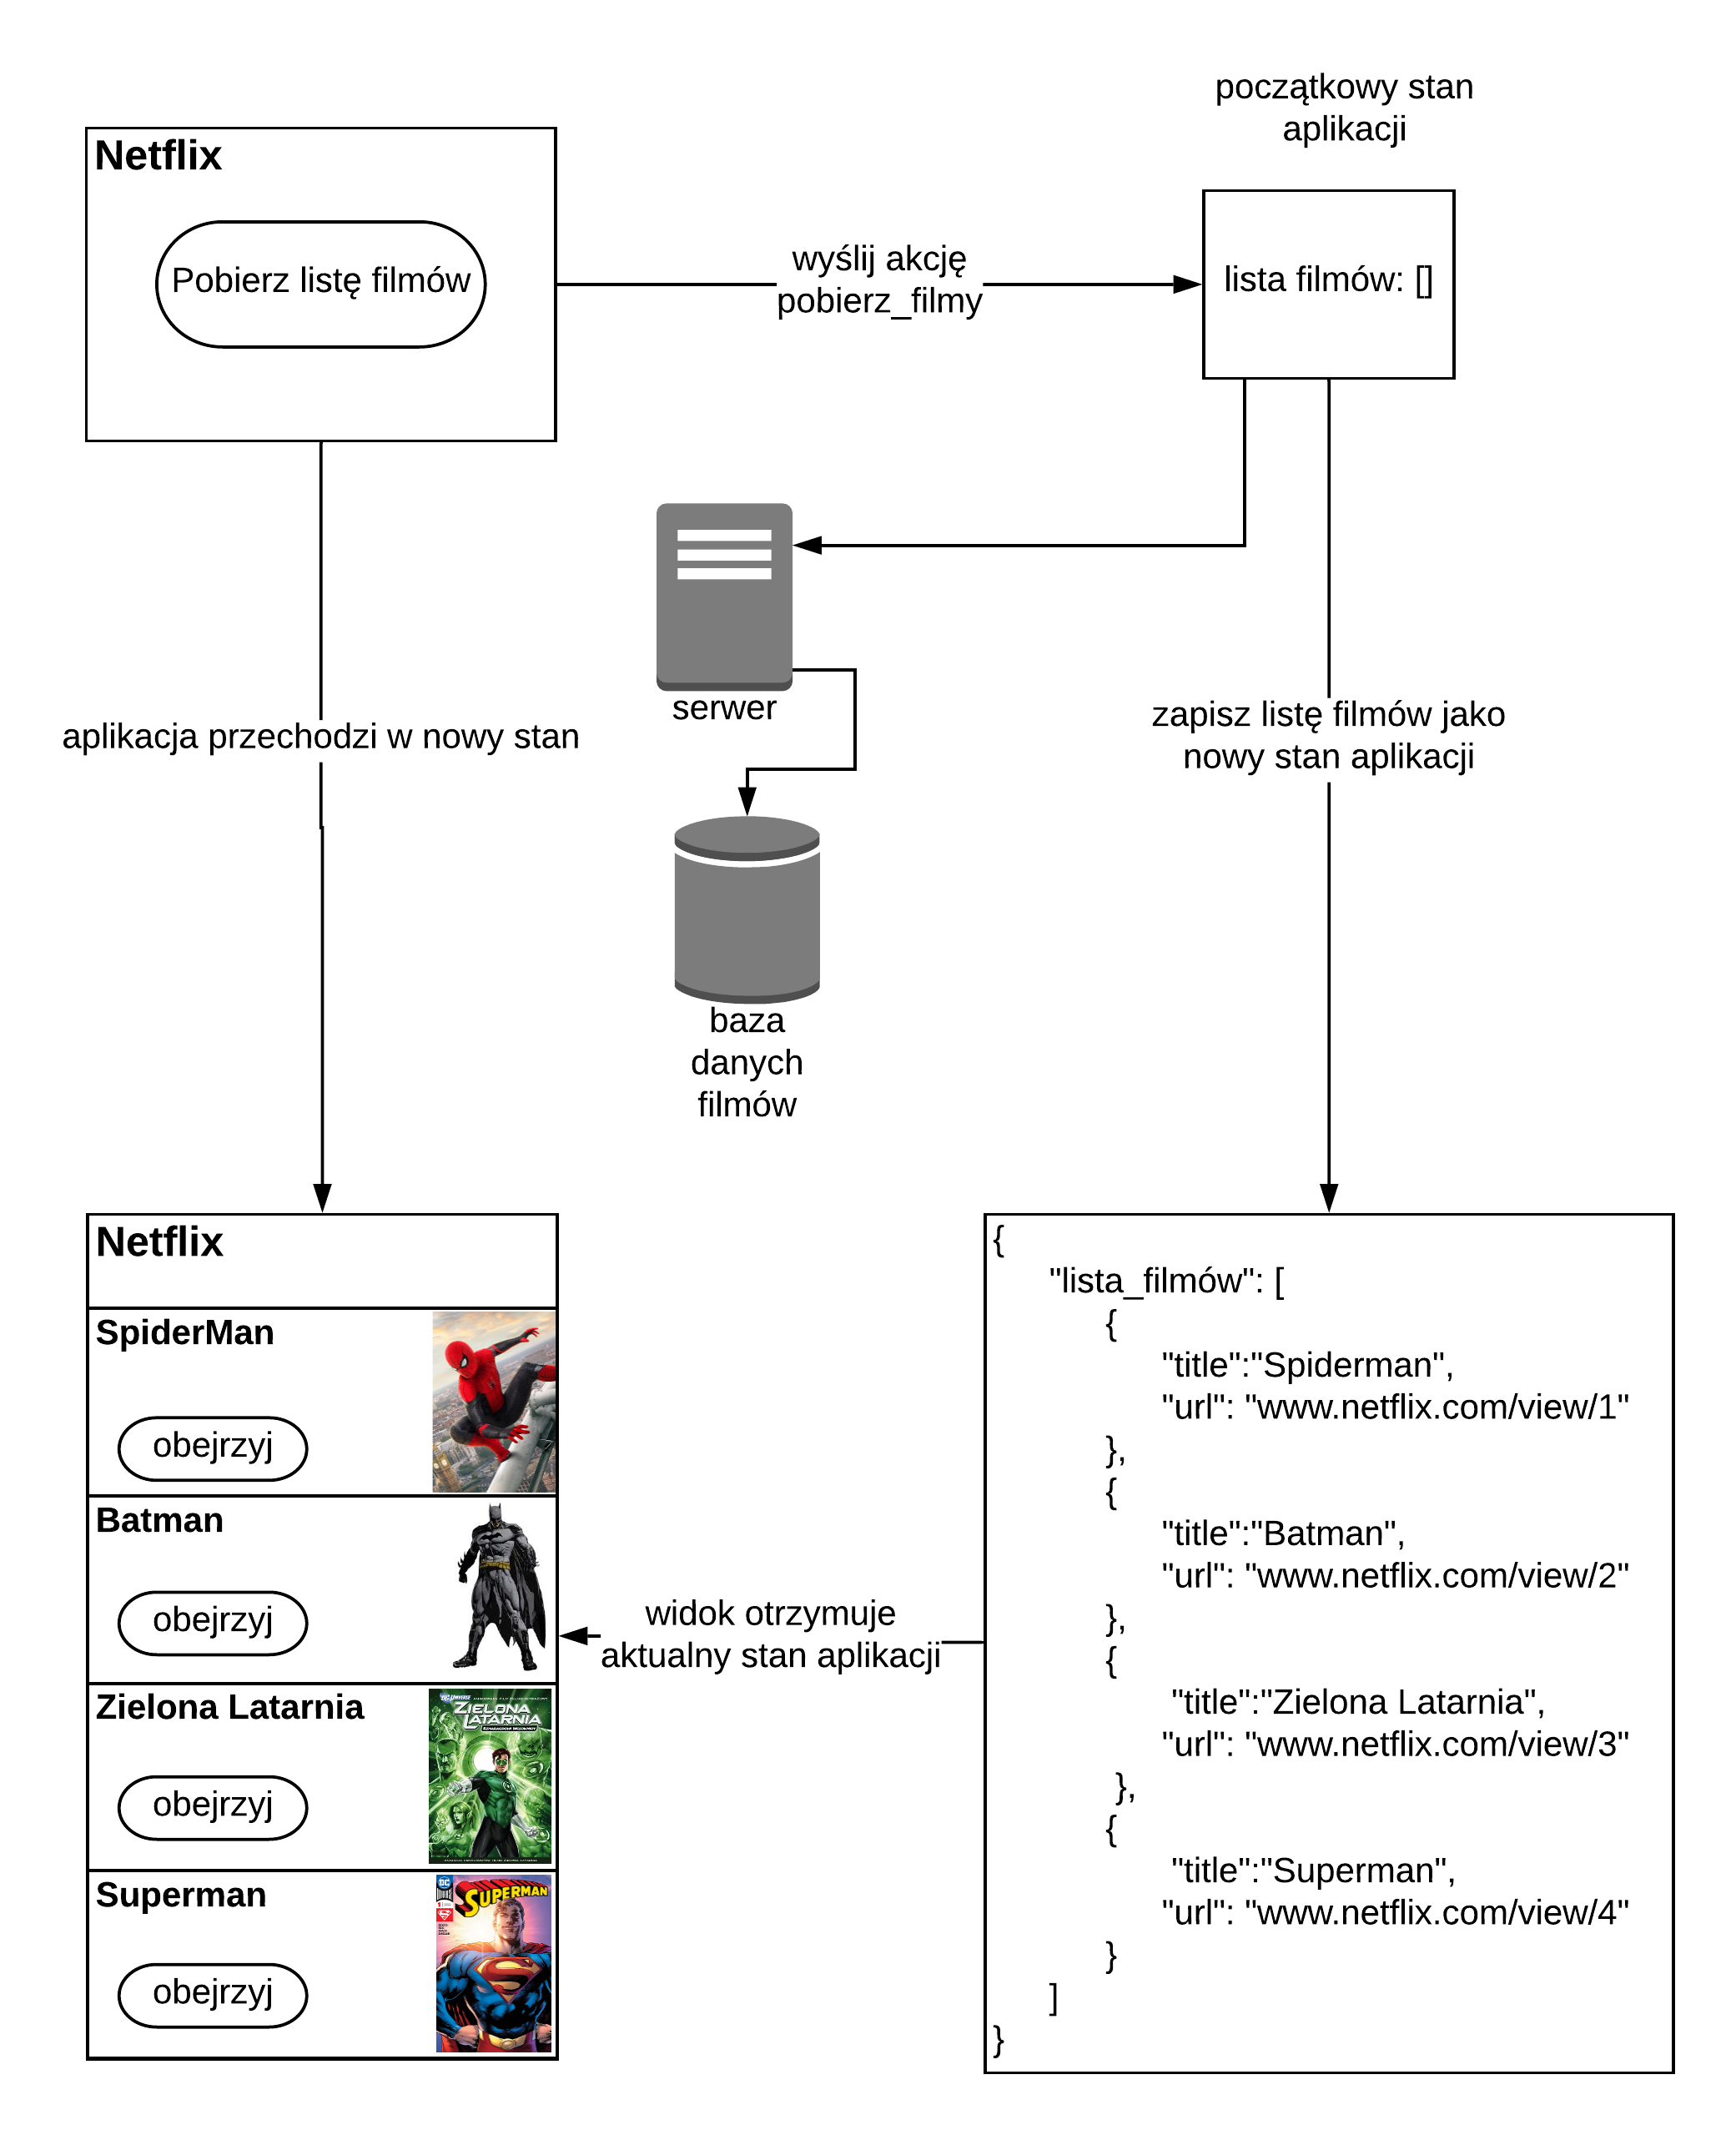
\includegraphics[width=20cm]{rysunek_9.png}
    \caption{Grafika przedstawiająca mechanizm działania aplikacji dynamicznych}
    \label{fig:rysunek_9}
\end{figure}

Aplikacja w stanie początkowym nie posiada żadnych filmów. Użytkownik klika przycisk pobierz listę filmów. Efektem ubocznym (side effect)  jest wysłanie informacji o akcji do menedżera stanu.
Menedżer stanu wysyła zapytanie do serwera o listę filmów do zaproponowania. Serwer odpowiada z danymi, i menadżera stanu przechodzi w nowy stan.
Podstrona otrzymuje informacje o nowym stanie. Pobiera nowy stan z menedżera stanu i prze renderuje widok.

Problem pojawia się gdy chcemy określić kiedy cała procedura została zakończona.
Samo sprawdzenie czy przycisk został naciśnięty nie jest wystarczające, gdyż z perspektywy użytkownika, procedura obejmuje także rezultat efektu ubocznego.
Zapytanie do serwera zajmie od kilkudziesięciu milisekund do nawet i kilku czy kilkunastu sekund.
Samo renderowanie także nie jest deterministyczny w kontekście czasu operacji gdyż wpływ na nie mają inne usługi korzystające z procesora czy pamięci komputera.
Z racji, iż frameworki internetowe muszą być generyczne, nikomu jeszcze nie udało się stworzyć idealnego i jednolitego mechanizmu wyznaczania, czy dana akcja została zakończona czy nie.

Tak więc na potrzeby pracy istotnym jest, wprowadzenie jednoznacznej definicji akcji w aplikacji.

\emph{Akcja aplikacji - jest to zbiór procedur oraz zdarzeń i ich obsługi następujący w chwili interakcji użytkownika z aplikacją.}



\section{Specyfikacja wymagań}

W celu przeprowadzenia doświadczenia mającego na celu pomiar wydajności frameworków, należy posiadać odpowiednie środowisko badawcze.
Jak pokazano w przeglądzie istniejących rozwiązań, na rynku brak jest narzędzi pozwalających na przeprowadzenie pełnego i dokładnego badania.

Na potrzeby pracy stworzono narzędzie do rozwiązania zadanego problemu badawczego. W ramach projektu, założono co następuje:

\begin{itemize}
    \item Narzędzie jest generyczne - nie zakładamy konkretnej technologii aplikacji tak, że każdy istniejący jak i przyszły framework może zostać przebadany
    \item Stworzona zostanie ujednolicona lecz generyczna metoda dodawania nowej aplikacji do puli już istniejących
    \item Narzędzie musi posiadać obsługę różnych typów akcji aplikacji
    \item Narzędzie musi potrafić działać w odizolowanym środowisku (docker)
    \item Narzędzie będzie zautomatyzowane w znacznym stopniu
    \item Narzędzie będzie składać się z modułów tak, aby było łatwo rozwijalne w przyszłości
    \item Narzędzie pozwala na stworzenie różnych zestawów testów tak, aby użytkownik mógł dokładnie przebadać różne warianty akcji aplikacji
    \item Stworzony zostanie moduł parsowania danych z badania tak, aby można było otrzymać ujednolicony format wyniku
    \item Stworzony zostanie moduł wizualizujący wyniki
\end{itemize}

\section{Architektura rozwiązania}

Narzędzie które powinno powstać w celu rozwiązania tak skomplikowanego problemu nie jest łatwym zadaniem.
Na wstępie przedstawiono ogólny zarys architektury rozwiązania które spełnia wymogi przedstawione powyżej.
Z racji na obszerność rozwiązania, przedstawione zostanie ono w małych rozdziałach.

\subsection{Projekt testu wydajności}
Z założenia każda aplikacja którą chcemy porównać musi być zbudowana w możliwie zbliżony do siebie sposób.
Z racji, iż aplikacje internetowe są tworzone w sposób generyczny, istnieje mnogość możliwości implementacji każdego wymagania.
Innymi słowy, każde zadanie można wykonać na wiele różnych sposobów w ramach jednego narzędzia.
Każde rozwiązanie posiada swoje wady oraz zalety. Niektóre narzędzia pozwalają na dodatkową optymalizację kodu pod konkretne zadanie, pozwalając uzyskać jeszcze lepsze wyniki.
Niestety, mechanizmy takie polegają w znacznej mierze na zdolnościach i wiedzy programisty.
W ramach badania, chcemy porównać wydajność frameworków, a nie zdolności programisty, dlatego też aplikacje powinny zostać zaprojektowane w taki sposób, aby:
\begin{itemize}
    \item Były zdolne wykonać te same zadania
    \item Były możliwie proste
    \item Nie wymagały dogłębnej wiedzy programisty
    \item Posiadały ujednoliconą strukturę projektu
    \item Z racji, iż dla przeglądarki najtrudniejszym zadaniem jest renderowanie elementów
\end{itemize}
Test który zaprojektowano skupia się dokładnie na porównaniu wydajności renderowania dużej liczby elementów.

W tym miejscu warto odnieść się do świetnego artykułu autorstwa Pana Paula Lewisa \cite{rendering-performance} na temat optymalizacji renderowania w przeglądarce. Proces ten składa się z pięciu kroków przedstawionych na rysunku \ref{fig:rysunek_10}. 

\begin{figure}[]
    \centering
    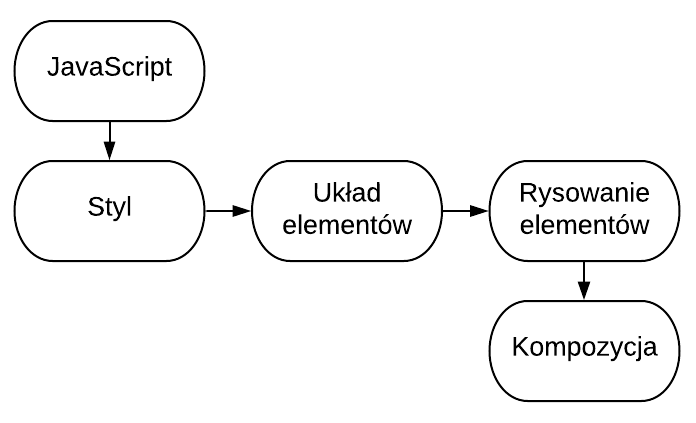
\includegraphics[width=12cm]{rysunek_10.png}
    \caption{Grafika przedstawiająca kolejność faz renderowania w przeglądarce \cite{rendering-performance}}
    \label{fig:rysunek_10}
\end{figure}

Na początku JavaScript wykonuje zmianę na dokumencie HTML.
Następnie przeglądarka wylicza na podstawie arkusza styli (CSS) pozycję elementów na płótnie przeglądarki.
Następnie znając rozmieszczenie elementów na stronie, przeglądarka wylicza ich wzajemne pozycje oraz rozmiar.
Elementy na stronie mają na siebie wzajemny wpływ na przykład dla dwóch bloków <li>.
W zależności od wysokości pierwszego bloku, drugi blok może zostać wyrenderowany, bądź też nie jeżeli wykracza on poza widoczny obszar rysowania, a także możemy wyliczyć dokładną pozycję na płótnie.
Znając pozycję oraz rozmiary elementów, przechodzimy do fazy malowania.
Pixele zostają malowane na wielu warstwach. W ostatniej fazie kompozycji, warstwy wyświetlone na ekran w konkretnej kolejności (odpowiada za to między innymi atrybut z-index w języku CSS).

Jak zostało przedstawione, renderowanie pojedynczej klatki na stronie jest bardzo skomplikowanym procesem, który w idealnym przypadku powinien następować około 60 razy na sekundę (w zależności od  częstotliwości odświeżania ekranu ).
Bardzo istotnym mechanizmem który przeglądarki stosuje w celu optymalizacji ilości pracy jest pomijanie niepotrzebnych fragmentów.
Jeżeli zmianie uległa tylko pewna część strony, na przykład kolor tekstu, możemy pominąć etap wyliczania layoutu strony.
Jeżeli nastąpi zmiana stanu, w której nie wystąpiła zmiana ani layoutu ani nie występuje potrzeba ponownego malowania, przeglądarka użyje poprzedniego zestawu gotowych warstw.
Zrozumienie tego mechanizmu jest istotnym czynnikiem na którym oparłem konstrukcję testów wydajnościowych.

Wracając do samej konstrukcji testu. Znając już mechanizm omijania czynności podczas renderowania obrazu w przeglądarce możemy przedstawić problem renderowania list.
Załóżmy, że mamy listę 20 wyrenderowanych elementów na stronie. Do listy możemy dopisać nowe wartości albo na początku albo na końcu.
W pierwszym kroku, dopisuję jeden nowy element do listy, na końcu co przedstawiono na rysunku \ref{fig:rysunek_11}. Każdy element na liście ma przypisany indeks.
Dopisując nowy element do listy, w optymalnym przypadku, powinienem wyrenderować tylko jeden nowy element i dokładnie tak się stanie. Co stanie się, gdy dopiszę nowy element na początku listy? Otóż wszystkie indeksy zostaną przesunięte o 1.
React wykryje zmianę jednego elementu na liście, i przeglądarka wyrenderuje tylko jeden nowy element . Widzimy także, że znaczna część fazy layoutu będzie taka sama, gdyż na ekranie zmieni się tylko jeden widoczny element.

\begin{figure}[]
    \centering
    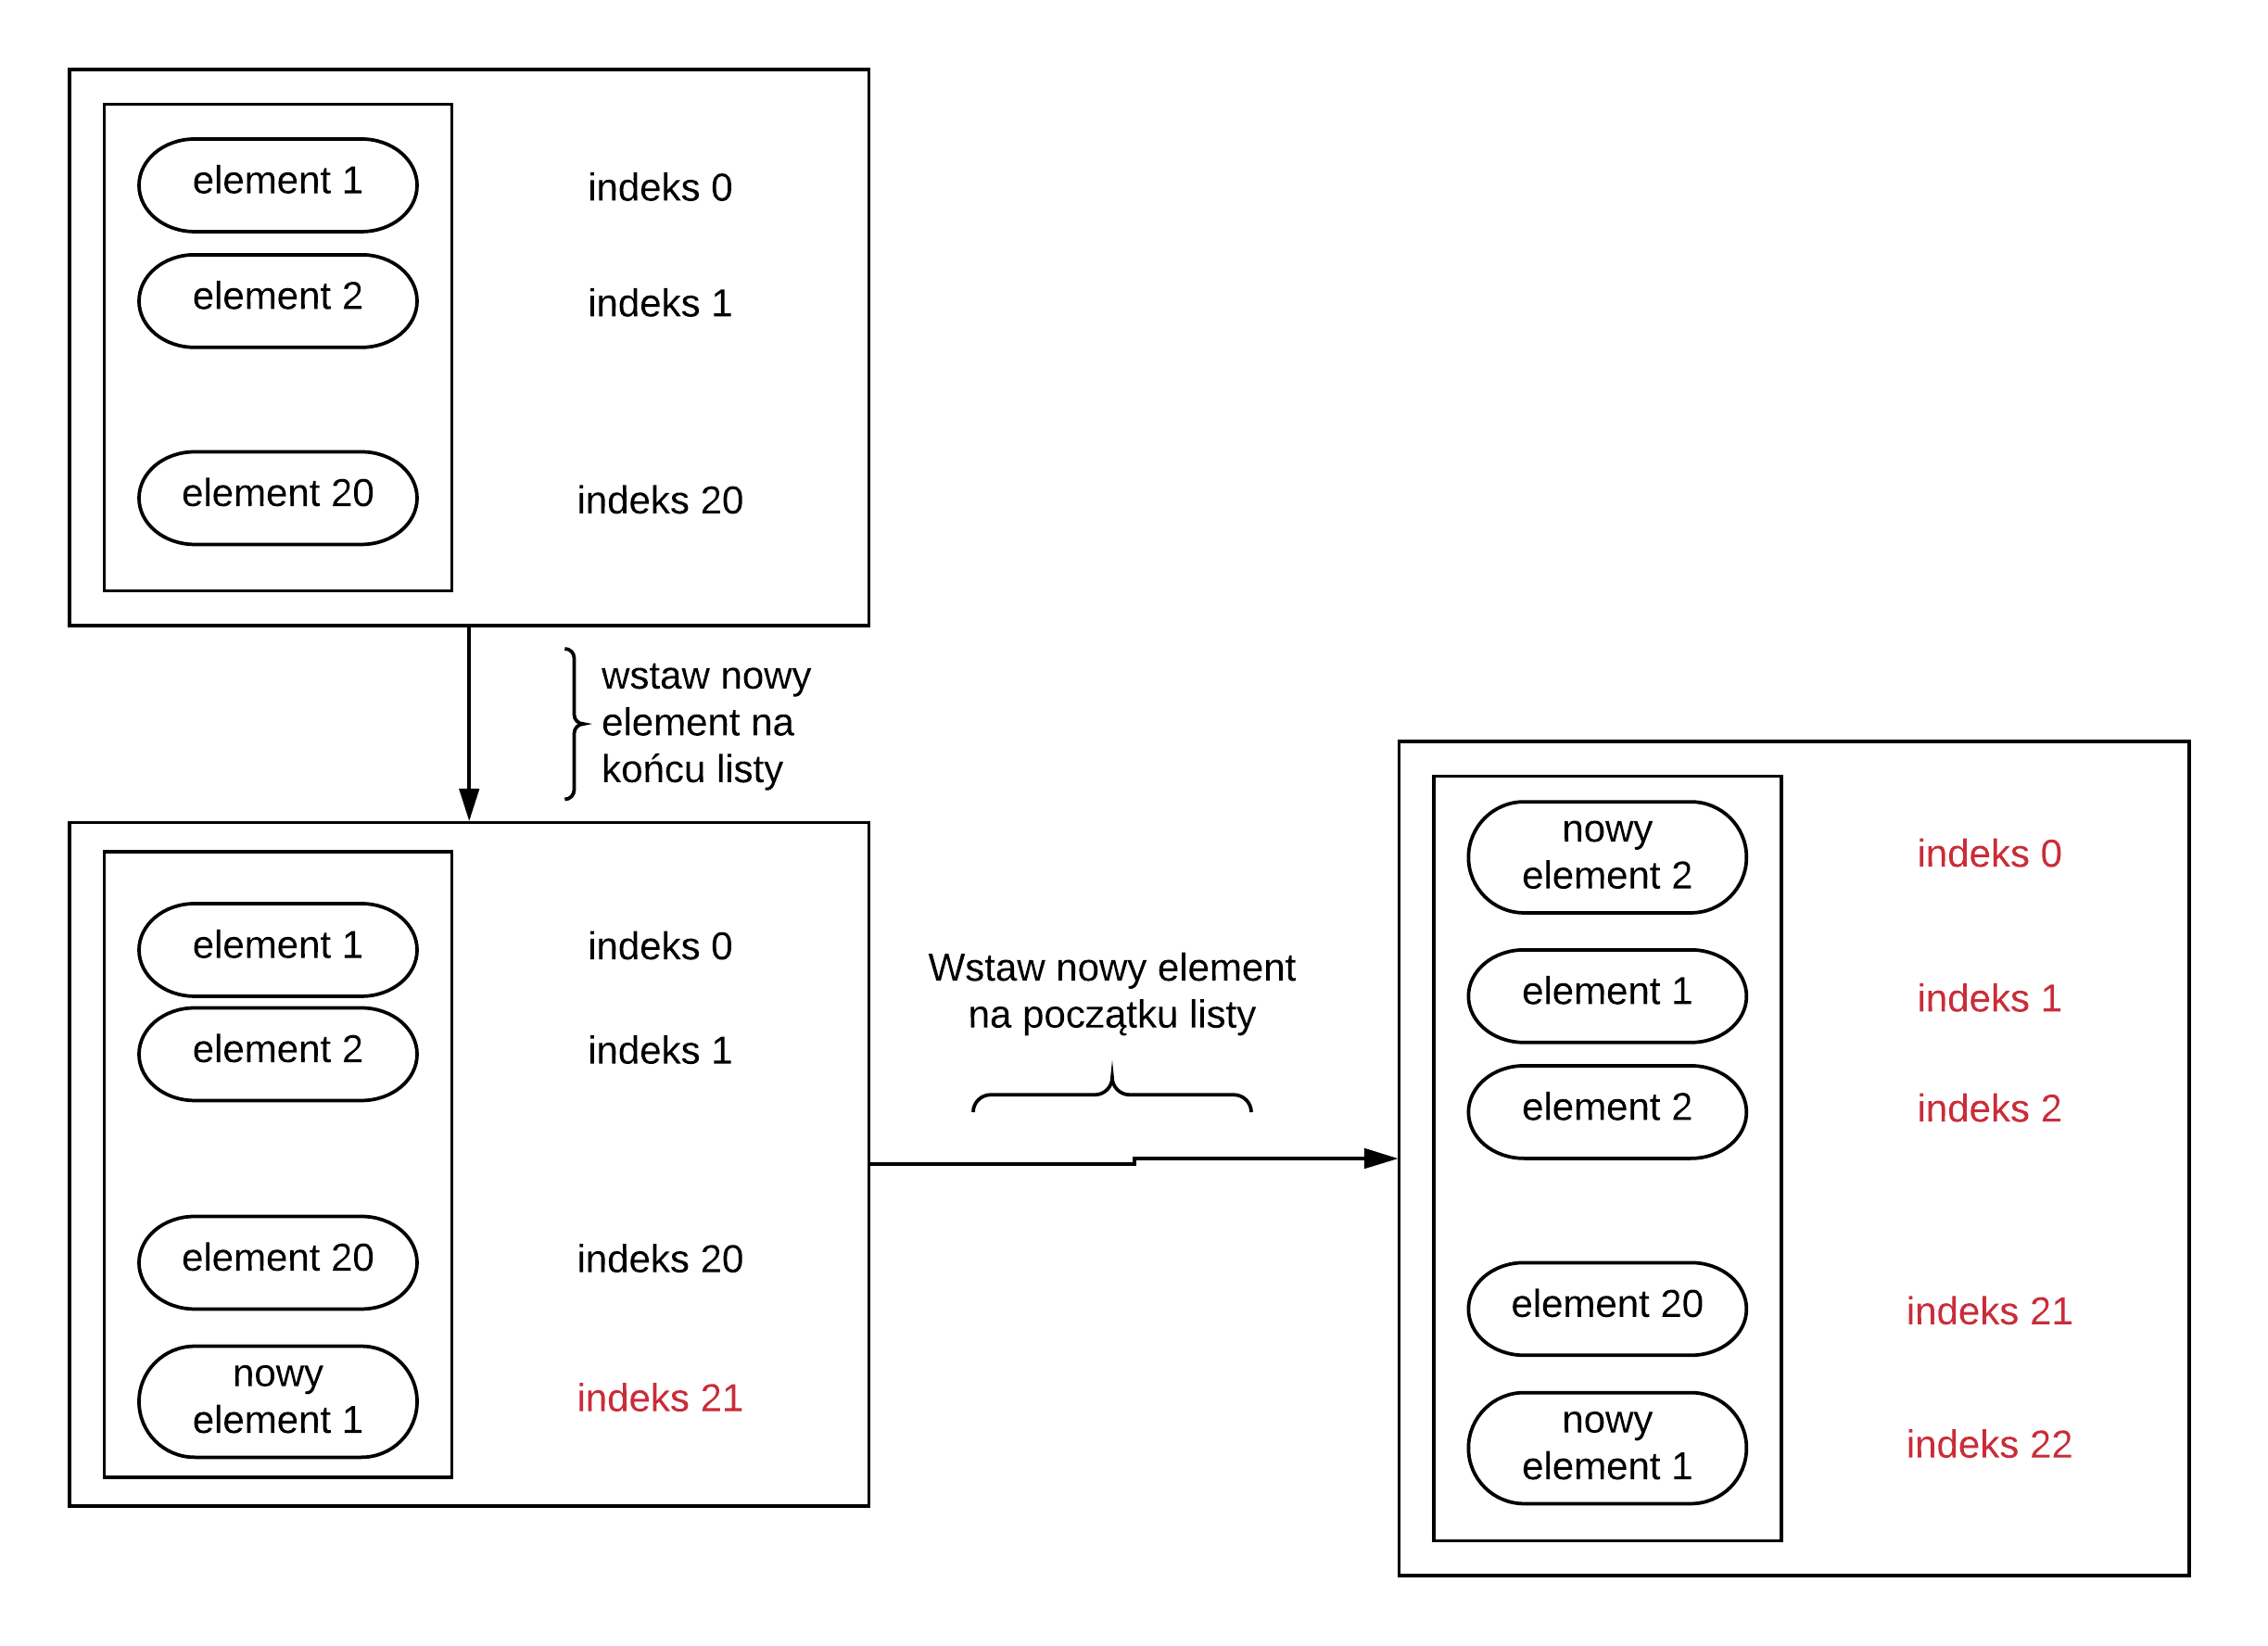
\includegraphics[width=16cm]{rysunek_11.png}
    \caption{Ilustracja przedstawiająca problem dopisywania elementu na koniec listy}
    \label{fig:rysunek_11}
    \vspace*{\floatsep}
    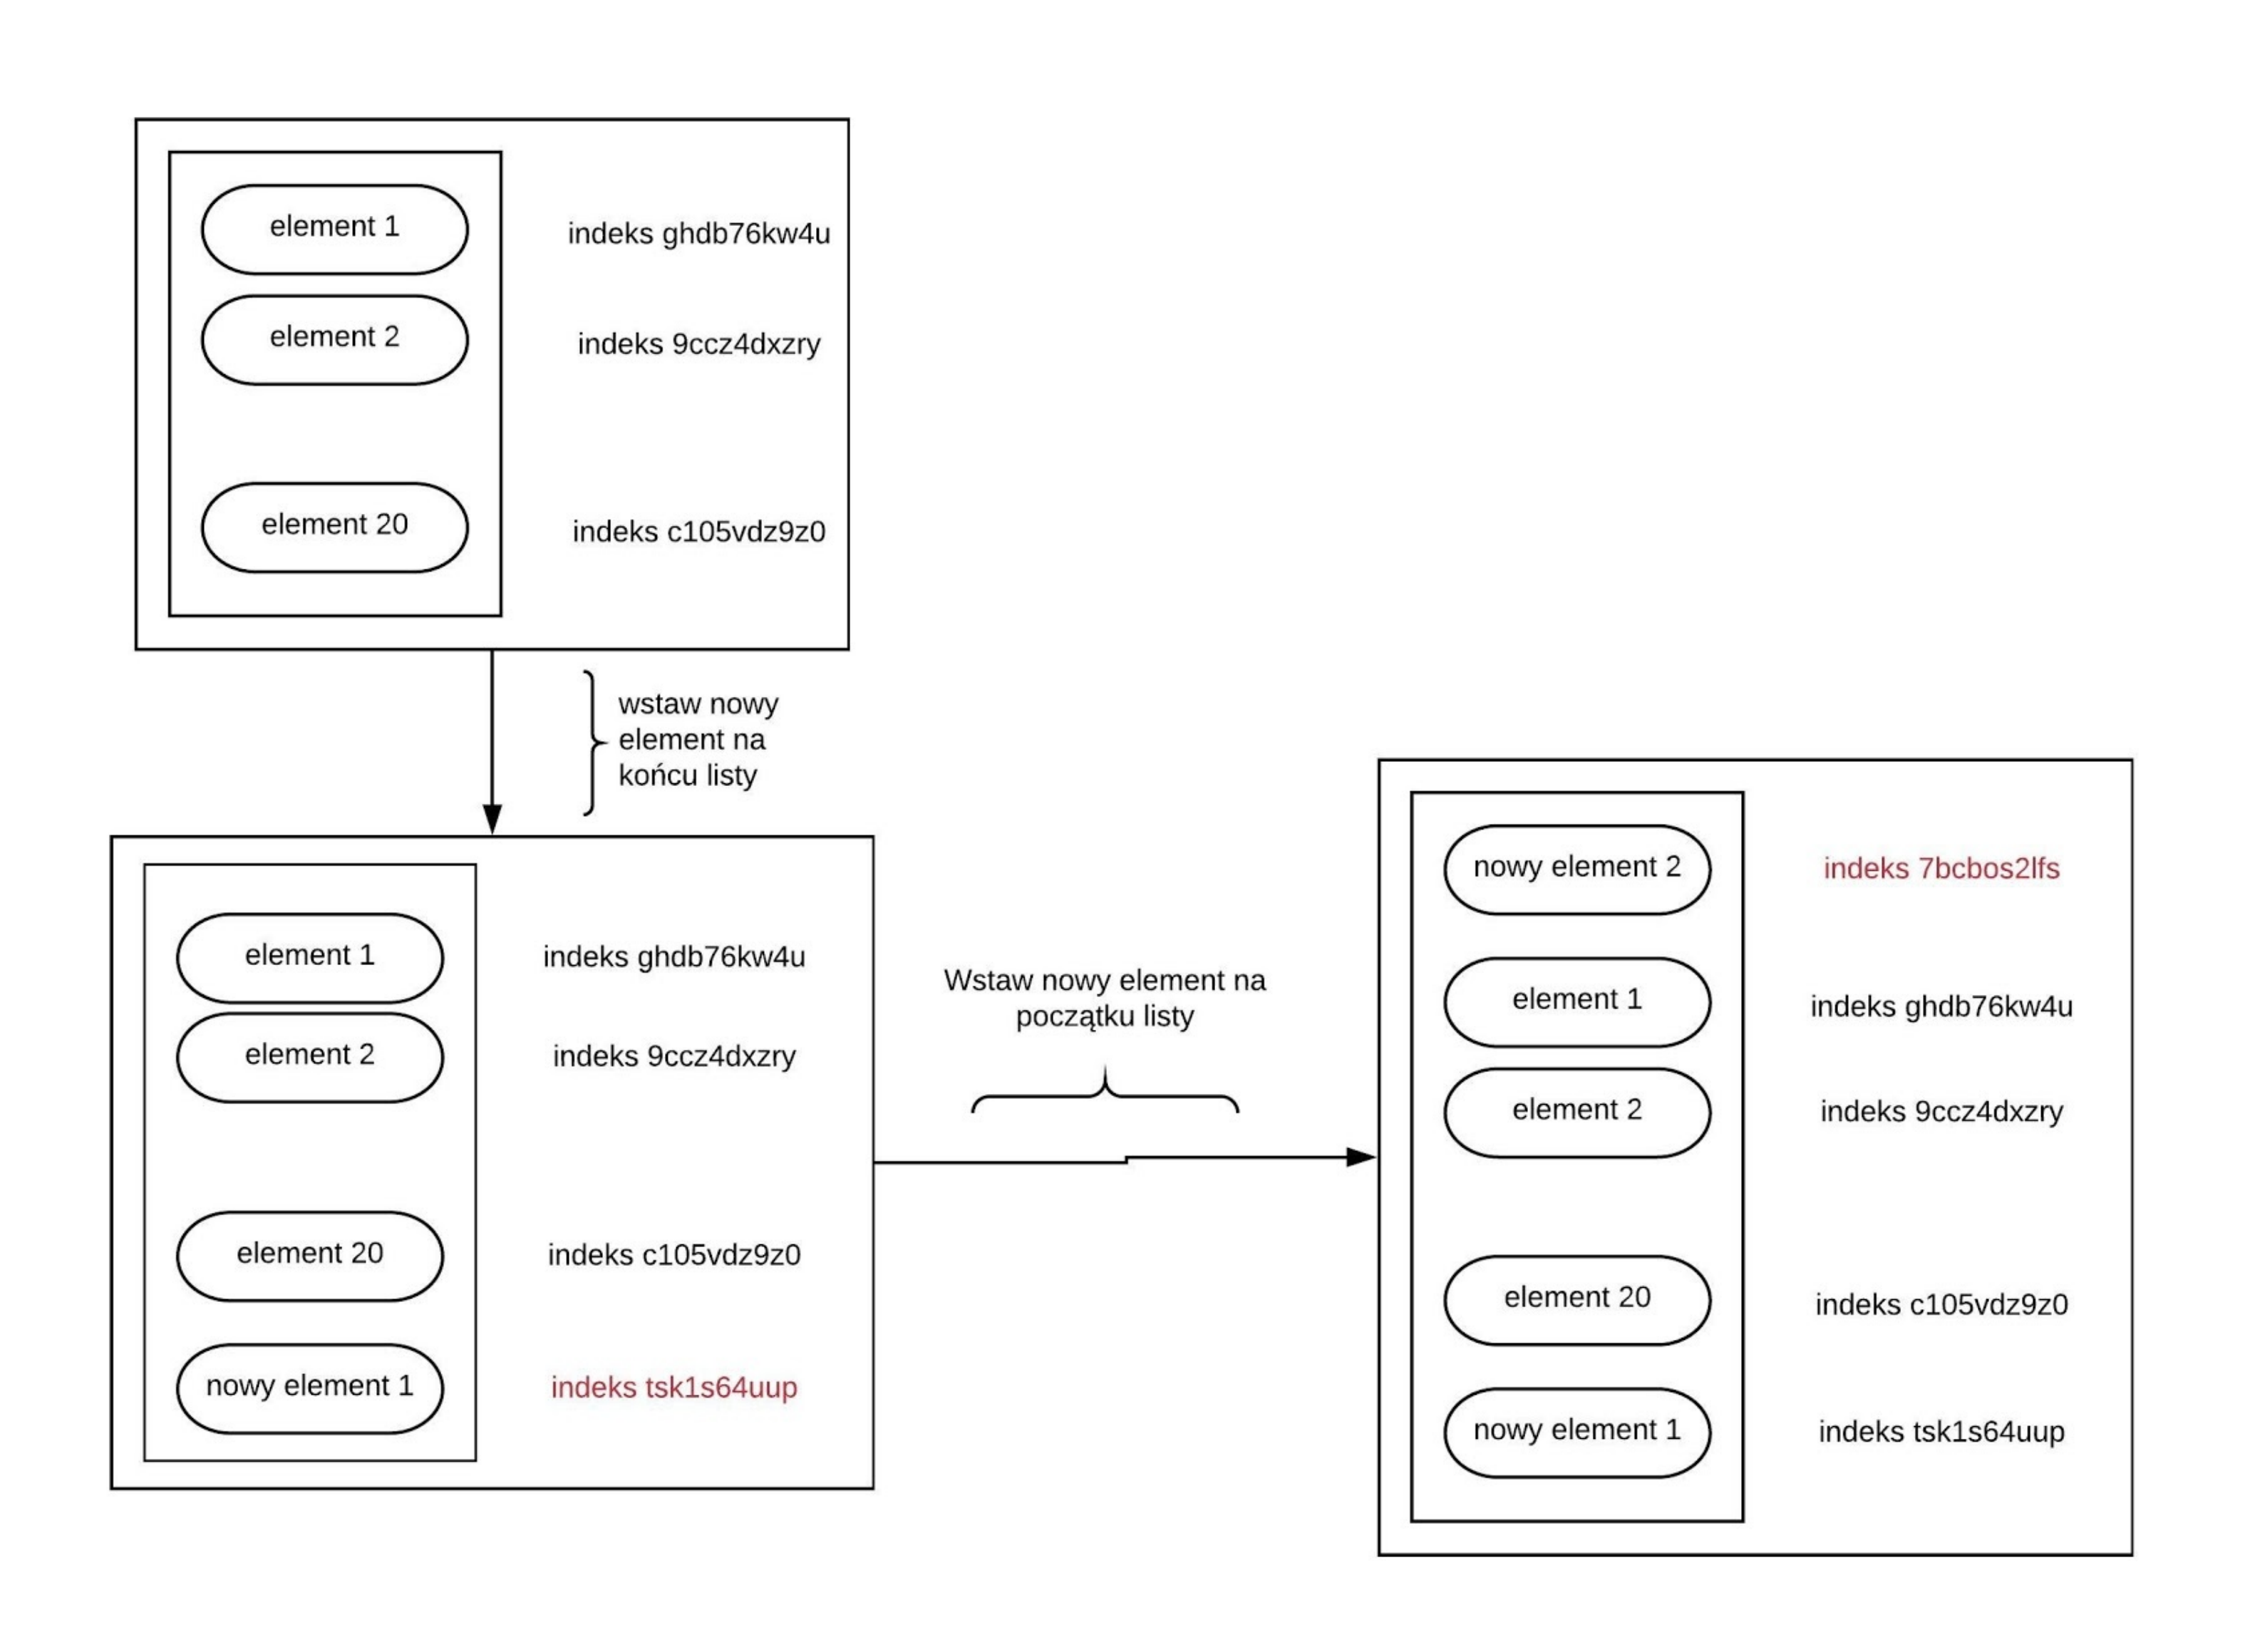
\includegraphics[width=16cm]{rysunek_12.png}
    \caption{Ilustracja przedstawiająca problem dopisywania elementów na początek listy}
    \label{fig:rysunek_12}
\end{figure}

Co stanie się w przypadku dopisania jednego nowego elementu na początku listy? Problem ten zaprezentowano na rysunku \ref{fig:rysunek_12}. Każdy indeks przypisany do elementu zostanie przesunięty o jeden.
Z racji tej, React ponownie wyrenderuje każdy element (gdyż uzna, iż jest to nowy element). Spowoduje to zmianę kodu HTML która zmusi przeglądarkę do pełnego prze renderowania wszystkich warstw oraz wyliczenia całego layoutu na nowo.
Oczywiście w skali 20 elementów które nie posiadają skomplikowanej struktury HTML i stylowania CSS nie powinno to robić problemu.
Jednak w dobie nowoczesnych aplikacji, listy (np lista filmów netflixa) posiadają masę małych elementów przez co lista nawet 50 elementów może spowodować zauważalne opóźnienia podczas użytkowania aplikacji.

W jaki sposób możemy poradzić sobie z tym problemem? Istnieją dwa sposoby dzięki którym React obiecuje znacznie wyższą wydajność w porównaniu do czystego kodu JavaScript.
Pierwszym z nich jest unikalny indeks elementu \cite{react-lists}. Zamiast stosować klucza równego indeksowi elementu, musimy podać klucz który jest unikalny w ramach elementu.
Przykładowo dla każdego elementu stworzymy parę (klucz, hasz). W tym momencie, jeżeli dodamy nowy element na początku listy, React spojrzy na listę kluczy, i zobaczy, że nie zmieniły się one, a dodano tylko jeden nowy element.
Zamiast 22 renredowań, otrzymamy tylko jedno.

Drugim sposobem poradzenia sobie z minimalizacją ilości renderowania jest koncepcja wirtualnego modelu DOM \cite{virtualdom}.
Jest to mechanizm, który tworzy reprezentację interfejsu użytkownika w pamięci i synchronizuje ją z modelem DOM przeglądarki. Proces ten nazywa się rekoncyliacją \cite{reconcilation}.
Pozwala to na wyrenderowanie tylko tych elementów, które różnią się między reprezentacją w pamięci a reprezentacją faktyczną drzewa DOM.

Znając już konkretny problem, z którym aplikacje SPA muszą się mierzyć, postanowiono zaprojektować szereg akcji manipulujących listą elementów oraz zbadać, ile czasu zajmie konkretnego frameworkowi wykonanie takiej czynności.

\subsection{Budowa aplikacji}

Każda aplikacja będzie składać się z szeregu przycisków. W wewnętrznym stanie aplikacji, będziemy trzymać listę wartości do wyrenderowania. Wartości które będziemy renderować będą stringiem o długości 10 znaków. Proces zmiany aplikacji prezentuję na poniższym rysunku.
\begin{figure}[htbp]
    \centering
    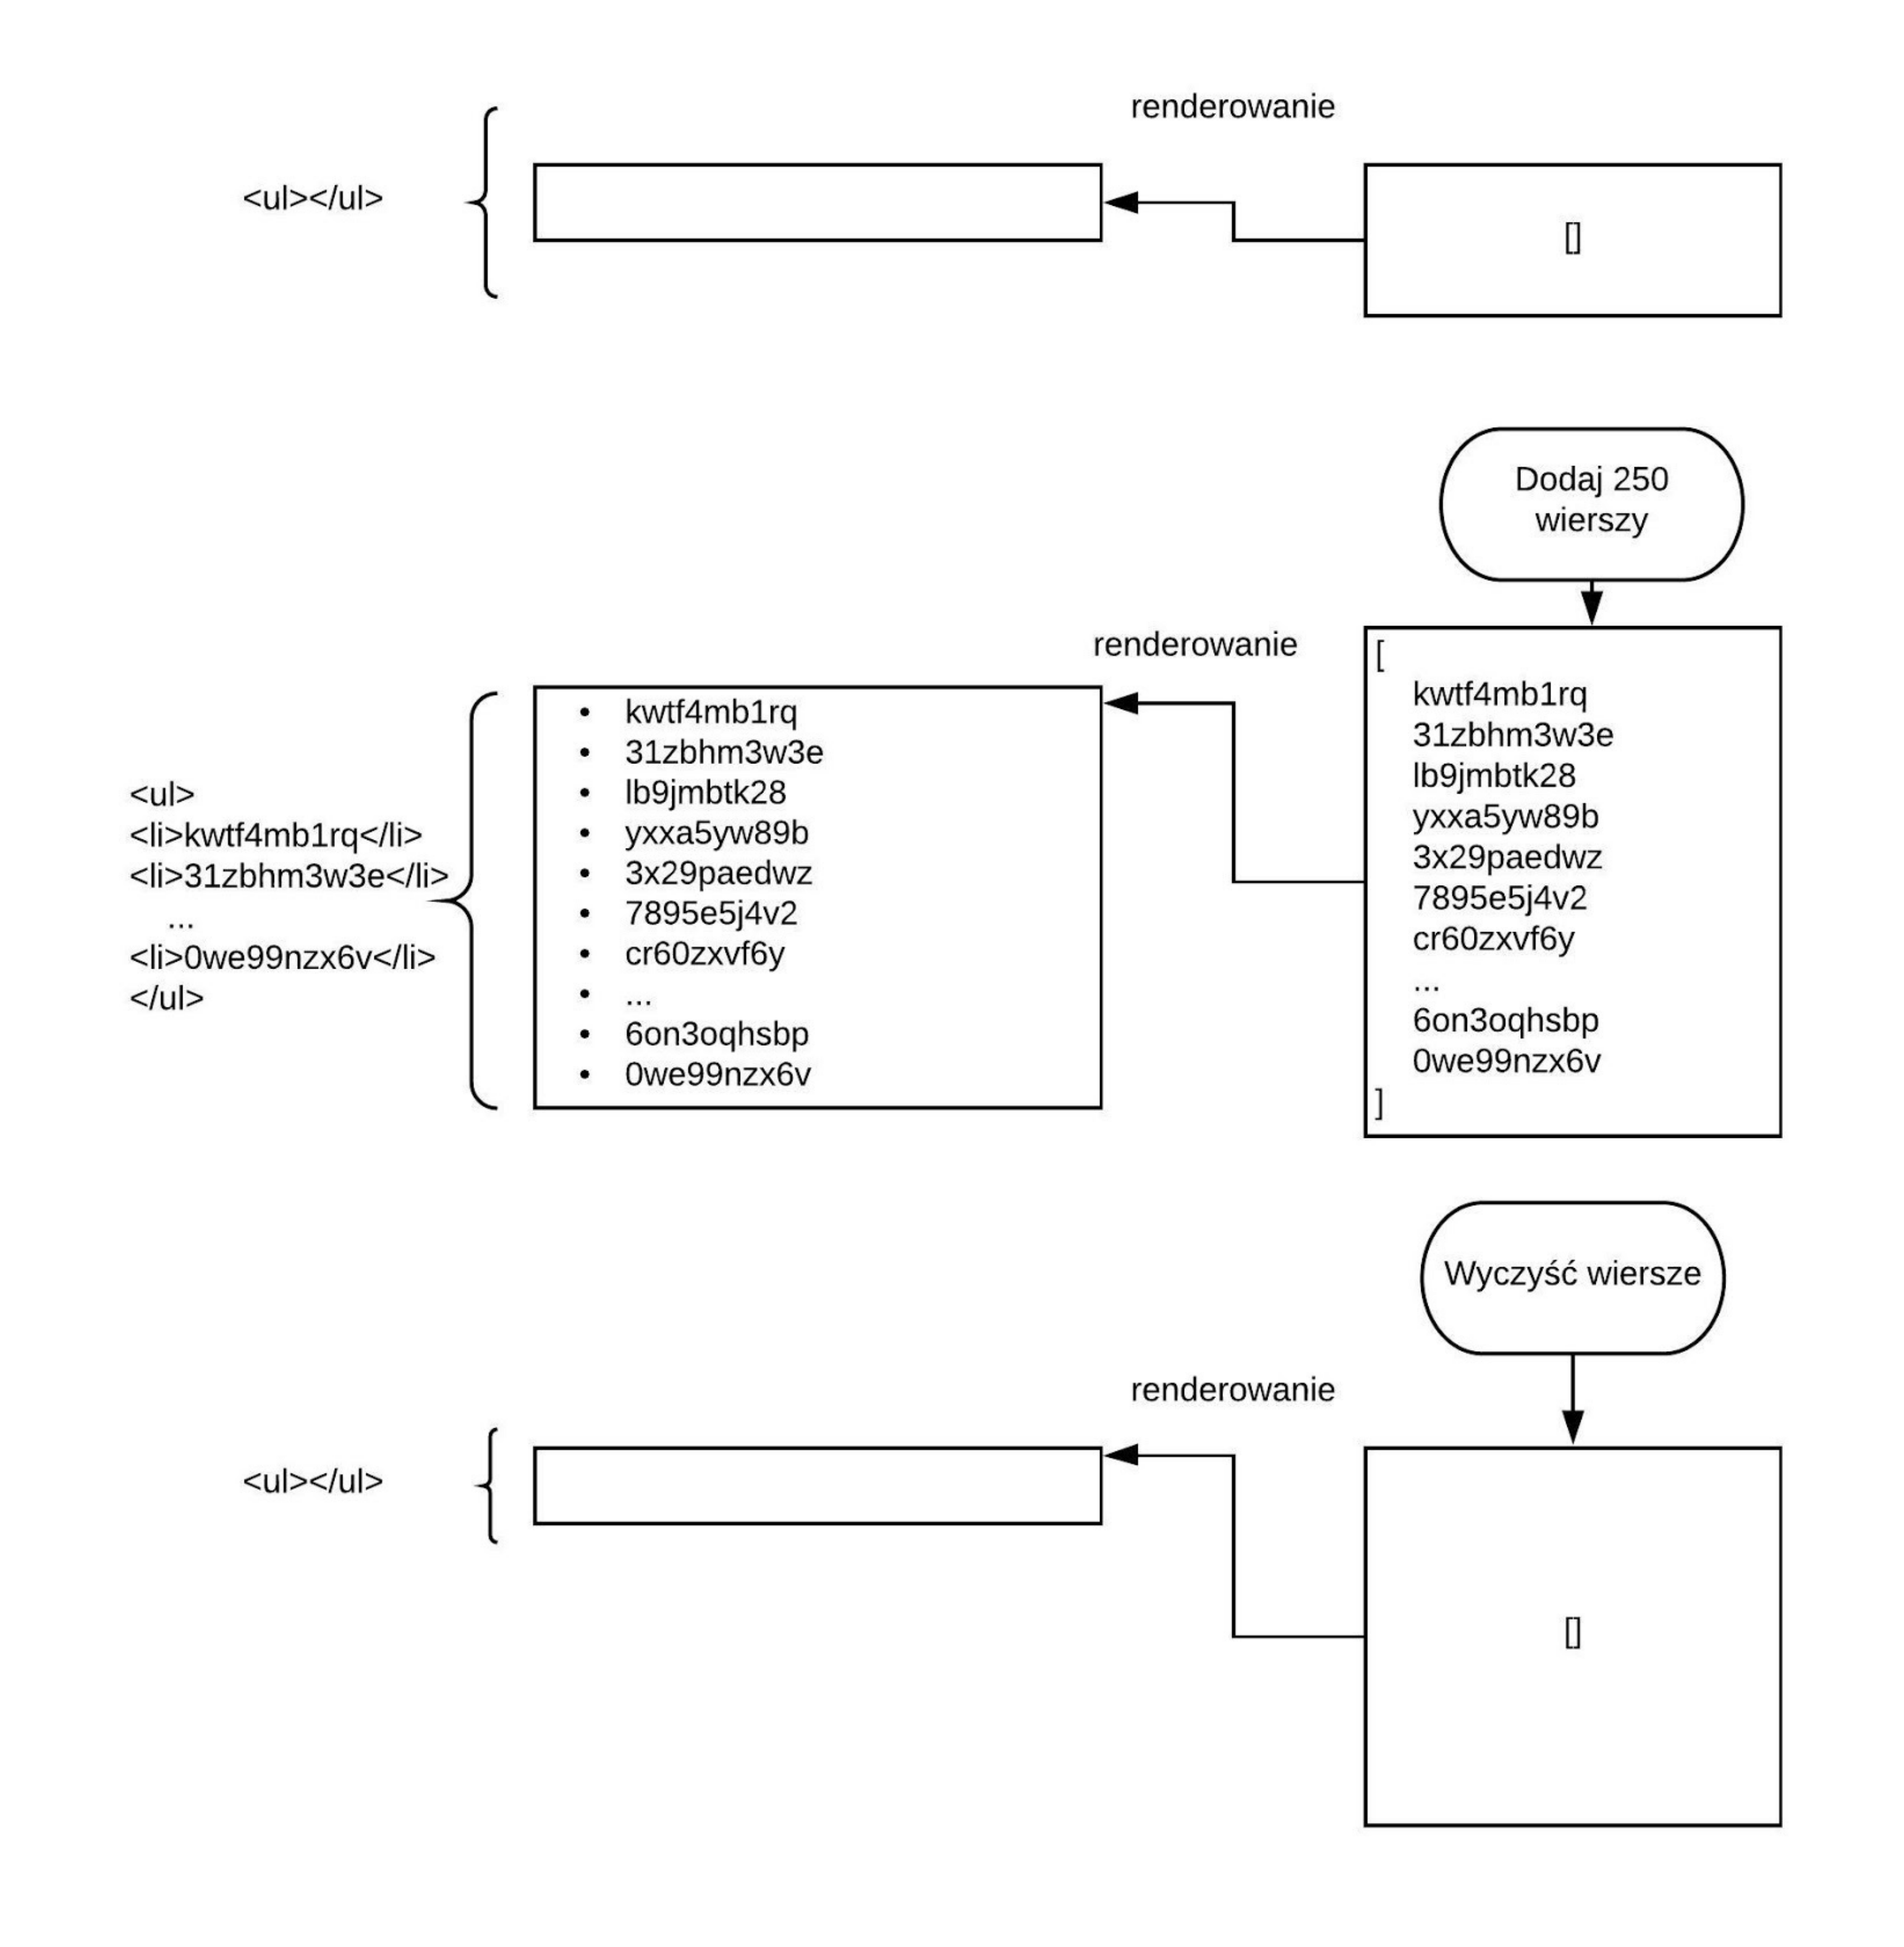
\includegraphics[width=\textwidth]{rysunek_13.png}
    \caption{Ilustracja mechanizmu przebiegu badania}
    \label{fig:rysunek_13}
\end{figure}

Na początku stan wewnętrzny aplikacji będzie pustą tablicą. Spowoduje to wyrenderowanie stanu minimalnego, czyli bloku <ul>.
Akcja naciśnięcia przycisku spowoduje wygenerowanie 250 wpisów zawierających wylosowane alfanumeryczne wartości. Wartości te muszą być, w miarę możliwości unikatowe.
Zmiana stanu z kolei spowoduje ponowne wyrenderowanie komponentu wyświetlającego listę. Kolejne akcje będą działać w myśl tej samej zasady.

Na rysunku poniżej przedstawiam listę akcji jakie aplikacja musi implementować:

\begin{figure}[htbp]
    \centering
    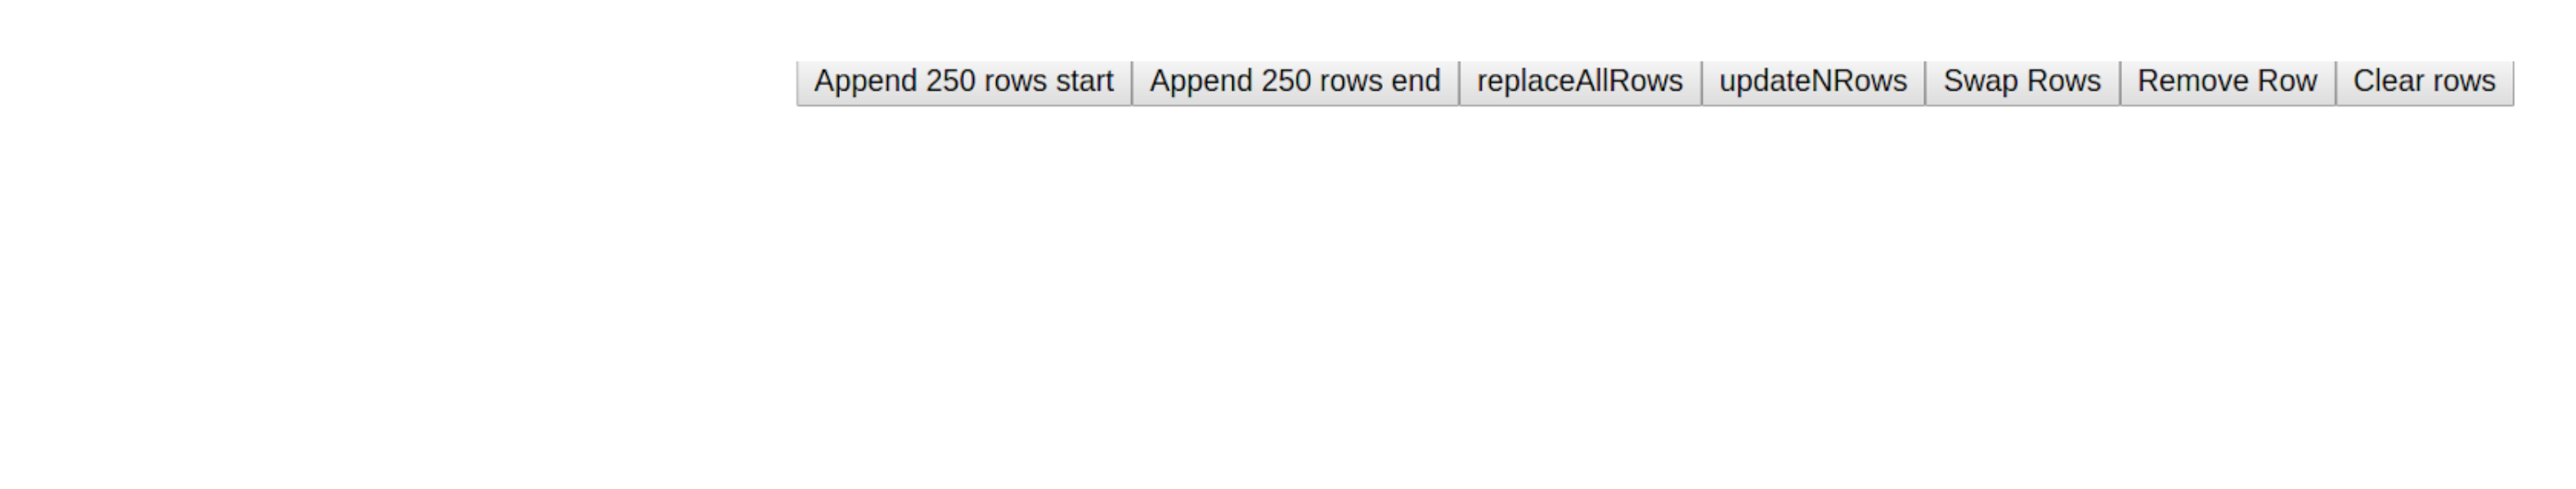
\includegraphics[width=\textwidth]{rysunek_14.png}
    \caption{Grafika przedstawiająca zaimplementowane przyciski w aplikacji}
    \label{fig:rysunek_14}
\end{figure}

\begin{itemize}
    \item \emph{Append 250 rows start} - dodaj 250 wierszy na początku listy
    \item \emph{Append 250 rows end} - dodaj 250 wierszy na końcu listy
    \item \emph{Replace all rows} - wygeneruj na nowo pełną listę wartości
    \item \emph{Update N rows} - wybierz losowo 250 wierszy i zaktualizuj ich wartości
    \item \emph{Swap rows} - zamień miejscami 2 wiersze
    \item \emph{Remove row} - usuń jeden wiesz
    \item \emph{Clear rows} - usuń wszystkie wiersze
\end{itemize}

Na początku części praktycznej wprowadzono definicję akcji aplikacji. Widzimy tutaj, iż samo przyciśnięcie przycisku dodania aplikacji nie jest wystarczające, gdyż przed wyrenderowaniem listy musimy wygenerować listę wpisów.
Renderowanie aplikacji także jest nie deterministyczne, i wpływ na nie ma szereg czynników niezależnych od przeglądarki.
Spowoduje to znaczne różnice w wynikach pomiaru czasu akcji aplikacji, z tego też powodu istotnym jest upewnienie się, iż kolejne iteracje badania są od siebie możliwie niezależne.

Ostatnim elementem składającym się na aplikację jest jej infrastruktura. Każda aplikacja tworzona jest w całkowicie inny sposób, dlatego istotnym jest, aby ujednolicić proces budowania i pakowania plików wynikowych.
Z racji tego, każda aplikacja musi posiadać w sobie plik Makefile \cite{gnu-makefile} z dwoma możliwymi celami:

\begin{itemize}
    \item install
    \item Production
\end{itemize}

Cel \emph{install} jak sama nazwa wskazuje, przygotuje folder \emph{node\_modules} zawierający pobrane biblioteki z platformy NPM \cite{npm}
Drugi cel \emph{production} zajmie się procesem pakowania aplikacji i optymalizacji kodu w celach produkcyjnych \cite{react-perf}.

\subsection{Przygotowanie aplikacji do badania}

Kolejnym krokiem podczas przygotowania aplikacji do badania, jest zautomatyzowanie procesu budowania i transferowania aplikacji. Przygotowujemy je tym samym do konteneryzacji \cite{kontenery}. W ramach tej części procesu, stworzono 3 skrypty.
\begin{itemize}
    \item Compile all applications - skrypt ten ma na celu przejście po wszystkich folderach aplikacji, i wykonanie komend install oraz production.Komendy wykonują szereg intensywnych zadań polegających na pobraniu dużej ilości danych a następnie transpilacji \cite{Transpilator} i optymalizacji kodu które są zadaniami wysoce obciążającymi procesor. Dlatego też przygotowanie aplikacji sekwencyjnie zajmuje dużo czasu i jest nieefektywne.
    Skrypt ten został zoptymalizowany aby wykonywał procesowanie współbieżne za pomocą mechanizmu obietnic \cite{promise}  w Javascript, dzięki temu w pełni wykorzystuje możliwości procesora.
    \item Copy released apps - Prosty skrypt mający na celu przekopiowanie folderu dist z każdej aplikacji do głównego folderu "releases".
    \item Create index html file - skrypt ten ma na celu stworzenie pliku index.html. W pliku tym zawrzemy informację o przygotowanych aplikacjach. Plik ten będzie dla nas istotny w dalszej części procesowania, gdy automat będzie wykrywać dostępne  aplikacje do badania.
\end{itemize}

Cały proces przedstawiony został na rysunku \ref{fig:rysunek_15}.

\begin{figure}[htbp]
    \centering
    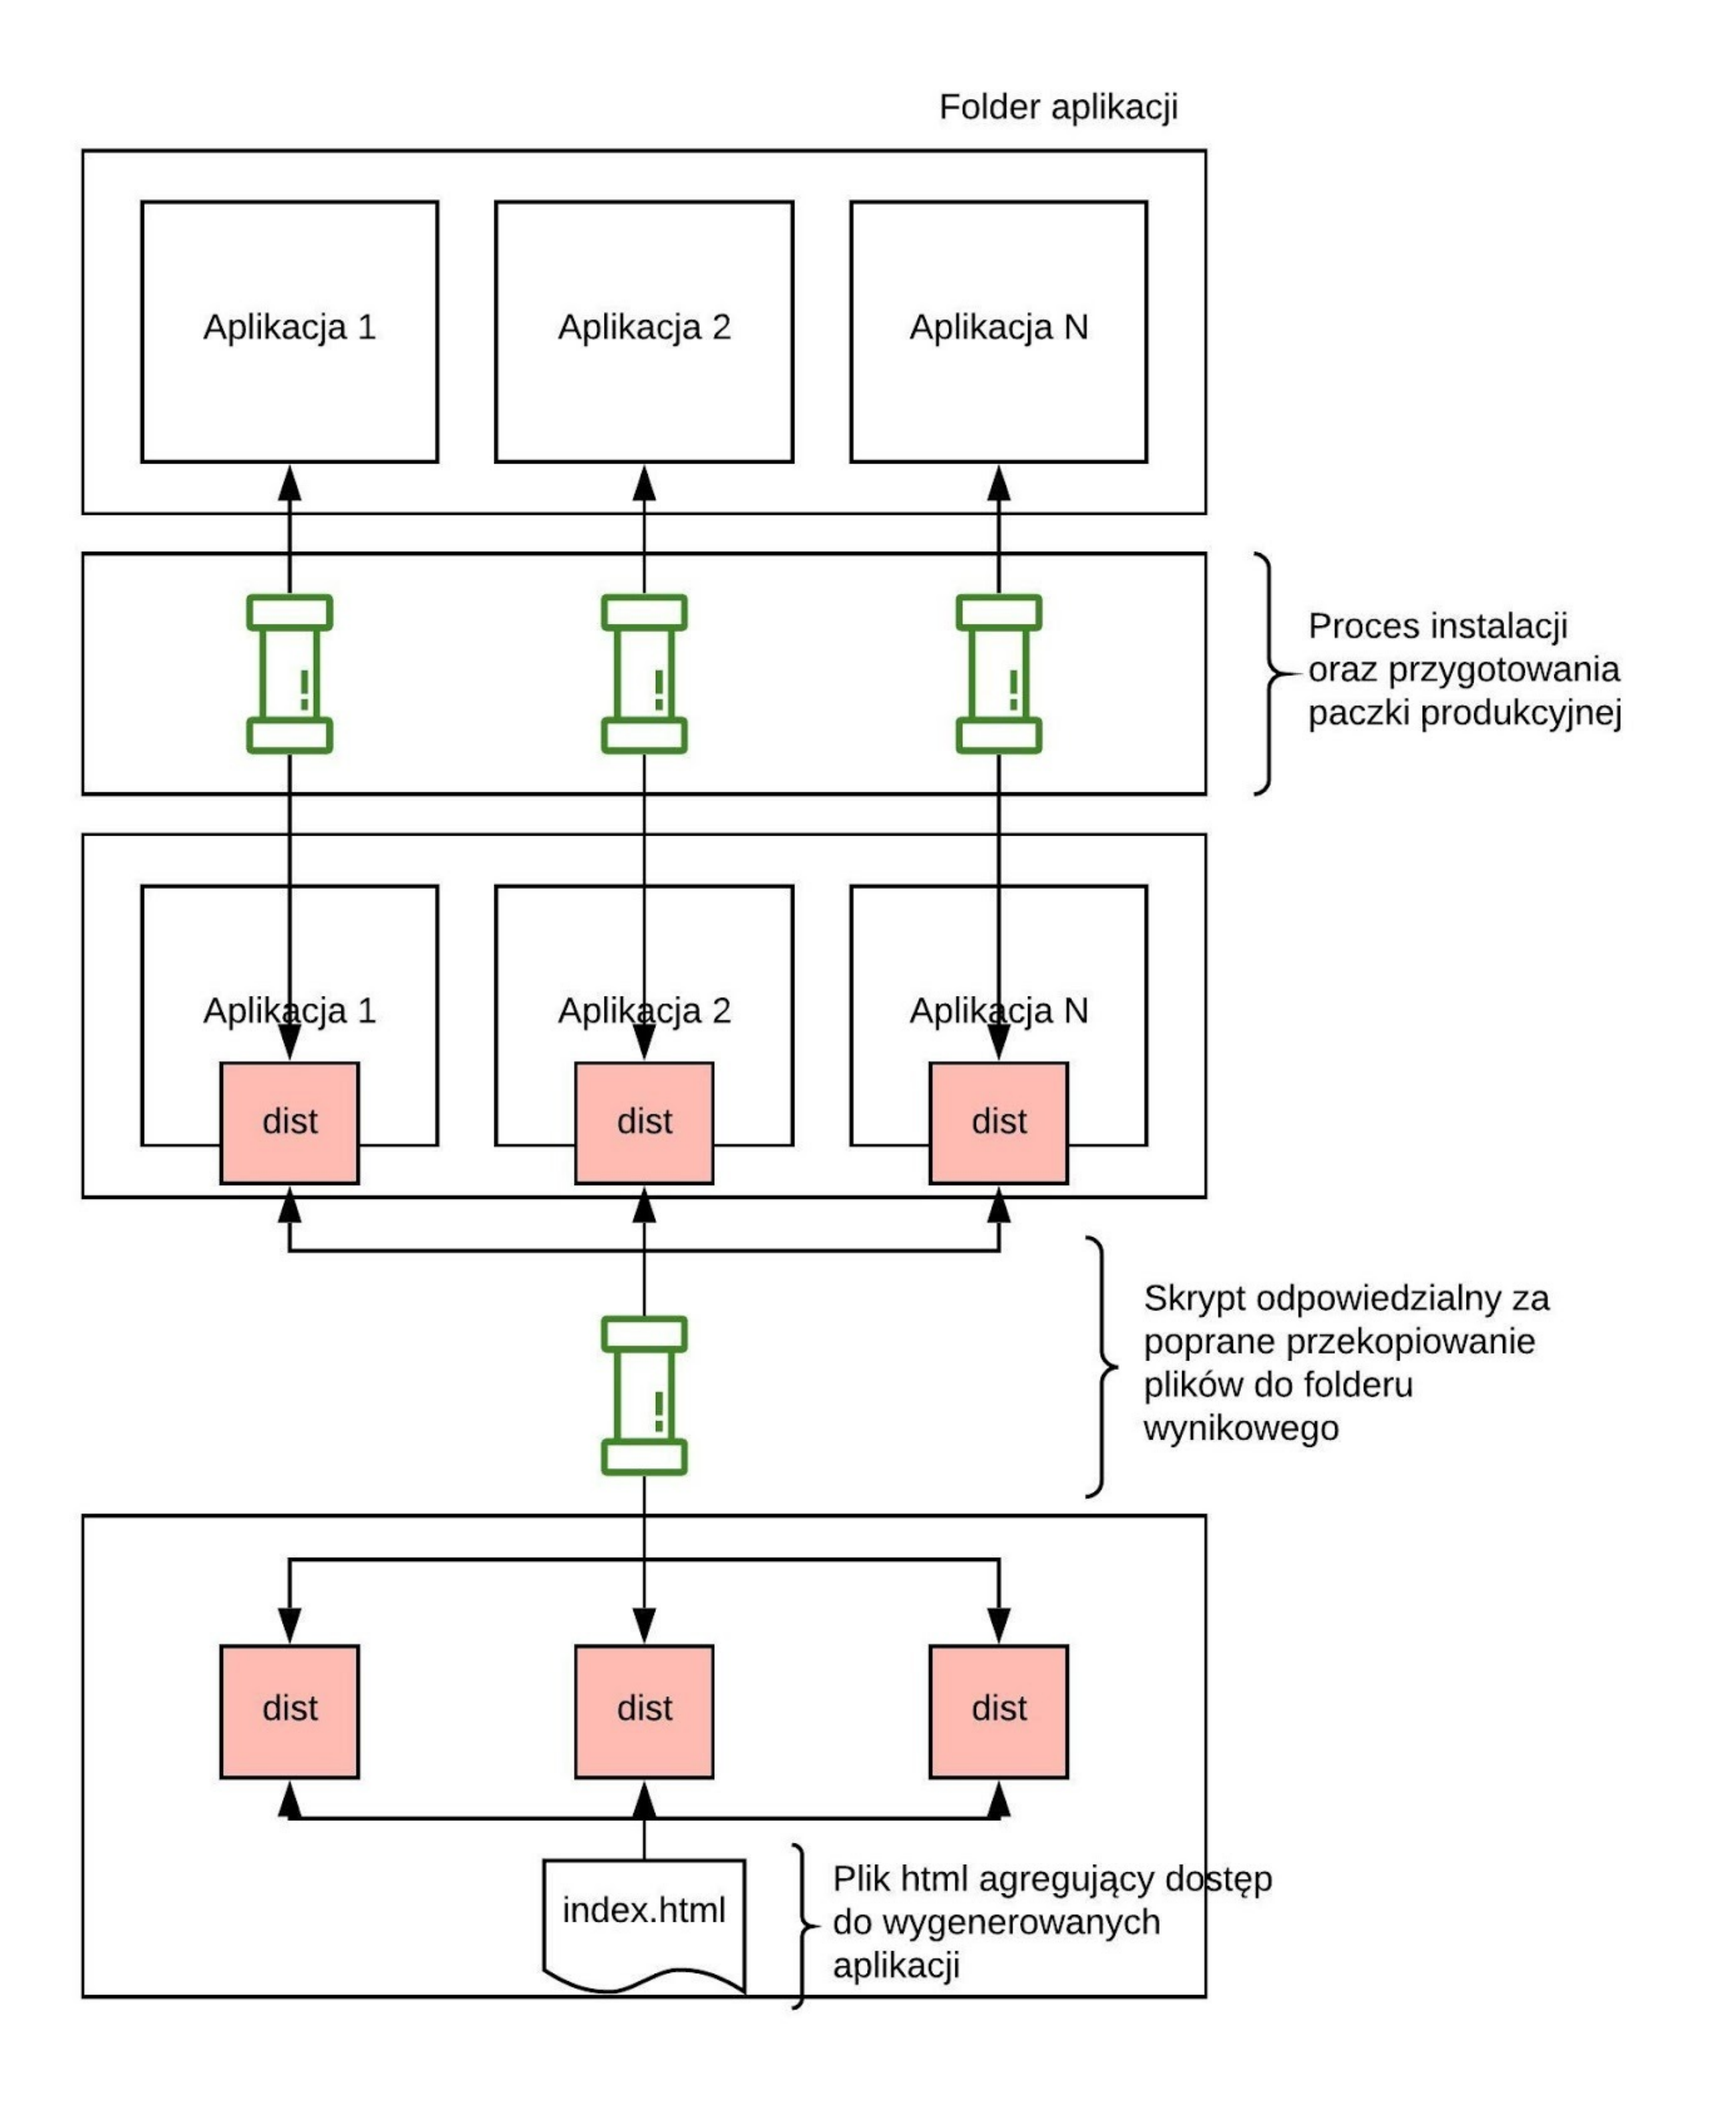
\includegraphics[width=\textwidth]{rysunek_15.png}
    \caption{Ilustracja procesu przygotowania aplikacji do konteneryzacji}
    \label{fig:rysunek_15}
\end{figure}

\subsection{Konteneryzacja aplikacji}

Na tym etapie, dysponuje już zbudowanymi paczkami aplikacji. Aplikacje zostały zoptymalizowany do produkcyjnego użytku. Dodatkowo posiadam plik index.html stanowiący punkt wejścia do dalszego procesowania.

Kolejnym krokiem jest stworzenie mechanizmu umożliwiającego dostęp do aplikacji. W normalnym środowisku służą do tego serwery aplikacji \cite{web-server}. Przykładem takiego serwera jest Nginx lub Apache.
Z racji, iż instalacja takich serwerów wiążę się z pobraniem dużej ilości danych oraz każdorazową konfiguracją środowiska, skonteneryzowane rozwiązania znacząco przyspieszy i uprości pracę.

Jednym z założeń narzędzia jest, aby całość działała w odizolowanym środowisku przy użyciu platformy docker \cite{docker}. W zależności od systemu operacyjnego, zestaw instrukcji potrzebnych do instalacji serwera może być całkowicie inny \cite{nginx-windows}\cite{nginx-linux}.
Dlatego też wykorzystanie odizolowanej warstwy abstrakcji nad systemem operacyjnym jest istotnym zabiegiem.

Istotnym detalem dotyczącym platformy docker jest jej zasada działania. Aplikacje składają się z warstw obrazów, co przedstawiono na rysunku \ref{fig:rysunek_16}.
Aby rozpocząć nasz własny obraz, należy wybrać obraz bazowy. W celu zmniejszenia wagi obrazów, zazwyczaj stosuje się obrazy czystych, okrojonych wersji systemu Linux.
Przykładem takiego obrazu jest obraz alpine \cite{docker-alpine}, który jest systemem Linux o wadze 5 MB. Następny obraz jako swoją bazę wykorzysta obraz alpine, i doda kolejną warstwę oprogramowania.
Możliwym jest także jako bazę nowego obrazu, wybranie pełnoprawnej wersji systemu Linux na przykład bazą może być Ubuntu \cite{ubuntu}.
Dzięki wykorzystaniu podejścia komponentowego, rozwiązanie to jest bardzo generyczne i pozwala na publikację tego samego oprogramowania na wiele różnych sposobów.

\begin{figure}[htbp]
    \centering
    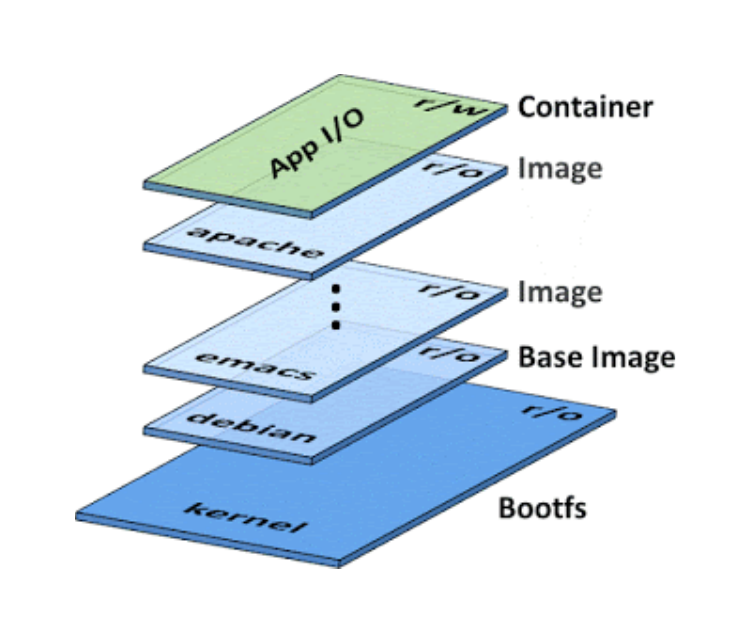
\includegraphics[width=10cm]{rysunek_16.png}
    \caption{Ilustracja przedstawiająca warstwy składające się na  przykładowy obraz dockera \cite{docker-layers}}
    \label{fig:rysunek_16}
\end{figure}

W celu stworzenia kontenera, należy utworzyć plik Dockerfile który jest plikiem typu YAML. W pliku tym precyzujemy, jaki obraz dockera ma być bazą naszego nowego obrazu.
Podczas pisania implementacji narzędzia, użyto obrazu \emph{nginx:1.17.6-alpine}. Następnie kopiowane są przygotowane w poprzednich krokach aplikacje do folderu \emph{/var/www}.
Jest to folder który NGINX wykorzystuje do serwowania plikóœ. Kolejny krokiem jest przygotowanie wcześniej stworzonego pliku nginx.conf jako pliku konfiguracyjnego serwera NGINX.
Prezycje się w nim wiele istotnych opcji, lecz dla nas jedyną inretesującą opcja jest ścieżka do folderu aplikacji, port oraz plik index.html. Następnie następuje etap budowy nowego kontenera.

Z racji, iż nowy kontener musi być zbudowany od nowa za każdym razem, gdy zmienimy kod aplikacji, stworzono plik Makefile mający na celu usprawnienie całego procesu.
Należy wykonać komendę \textbf{make\ build\_nginx\_image}.
Po zbudowaniu obrazu, możemy uruchomić nasz serwer za pomocą komendy \textbf{make\ start\_nginx\_docker}. Będzie on dostępny pod adresem \textbf{http://localhost:8085}.

Ostatnim elementem jest opisanie faktycznego wyniku całego procesu. W tym celu, wchodzimy na stronę \textbf{http://localhost:8085}. Naszym oczom ukaże się bardzo prosta strona startowa przedstawiona na rysunku \ref{fig:rysunek_17}.
Strona ta będzie potrzebna kolejnemu modułowi badawczemu opartemu na Selenium, w celu wykrycia, jakie aplikacje są dostępne do badania.

\begin{figure}[htbp]
    \centering
    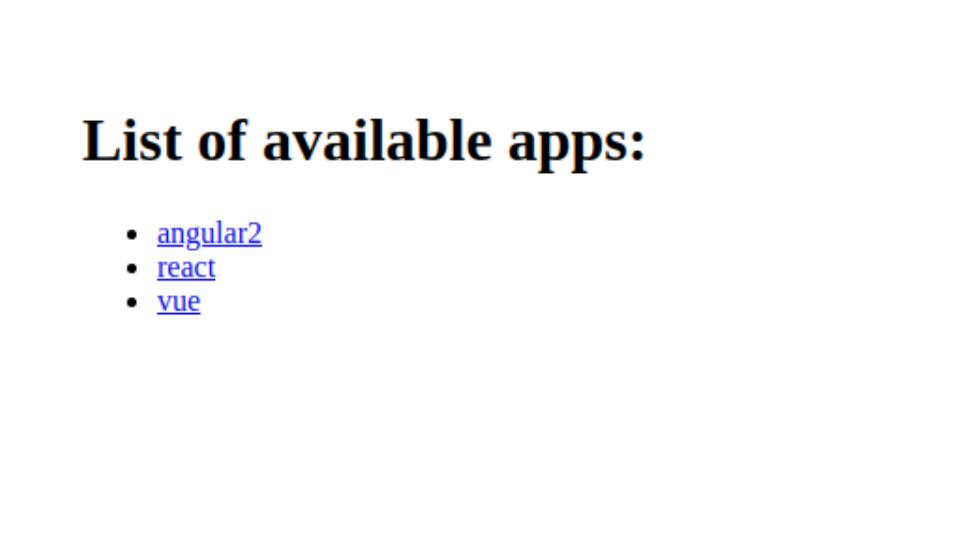
\includegraphics[width=10cm]{rysunek_17.png}
    \caption{Grafika przedstawiająca plik index.html wraz z dostępnymi aplikacjami do badania}
    \label{fig:rysunek_17}
\end{figure}

Możemy kliknąć na odnośnik przenoszący nas do konkretnej aplikacji.
Należy tylko pamiętać o poprawieniu portu, czyli aby przejść do implementacji reacta, należy wejść w link \linebreak \textbf{http://localhost:8085/react/}.


\subsection{Moduł badania}

Przechodzimy teraz do najbardziej skomplikowanego modułu całej pracy.
Mając już przygotowane aplikacje, wystawione do badania za pomocą serwera webowego, możemy w tym momencie zacząć interakcję z aplikacjami.
Nie mniej pojawia się duży problem pod tytułem, w jaki sposób możemy zacząć interakcję z aplikacjami?
Jak już wspomniano w poprzednich rozdziałach, akcje aplikacji są nie deterministyczne, co znacząco utrudnia możliwość badania takich aplikacji.
Ale na czym dokładnie polega problem?

W ramach pracy, posłużono się narzędziami powszechnie stosowanymi w celach testów end-to-end.
Ale najpierw, spójrzmy na problem z którym mamy do czynienia aby zrozumieć, jaki wpływ ma on na wyniki badania.

W statycznych aplikacjach internetowych, interakcja użytkownika ze stroną jest zazwyczaj bardzo uproszczona.
Znacząca większość akcji, będzie prowadziła do przeładowania treści strony (o czym mówiliśmy już w poprzednich rozdziałach pracy).
Zobrazowano to na przykładzie języka PHP na rysunku \ref{fig:rysunek_18}.

Oto najprostszy, wiekowy już przykład aplikacji kalendarza napisanej w PHP. Gdy będziemy chcieli zmienić miesiąc z marca na kwiecień, nastąpi przeładowanie całej strony.

\begin{figure}[htbp]
    \centering
    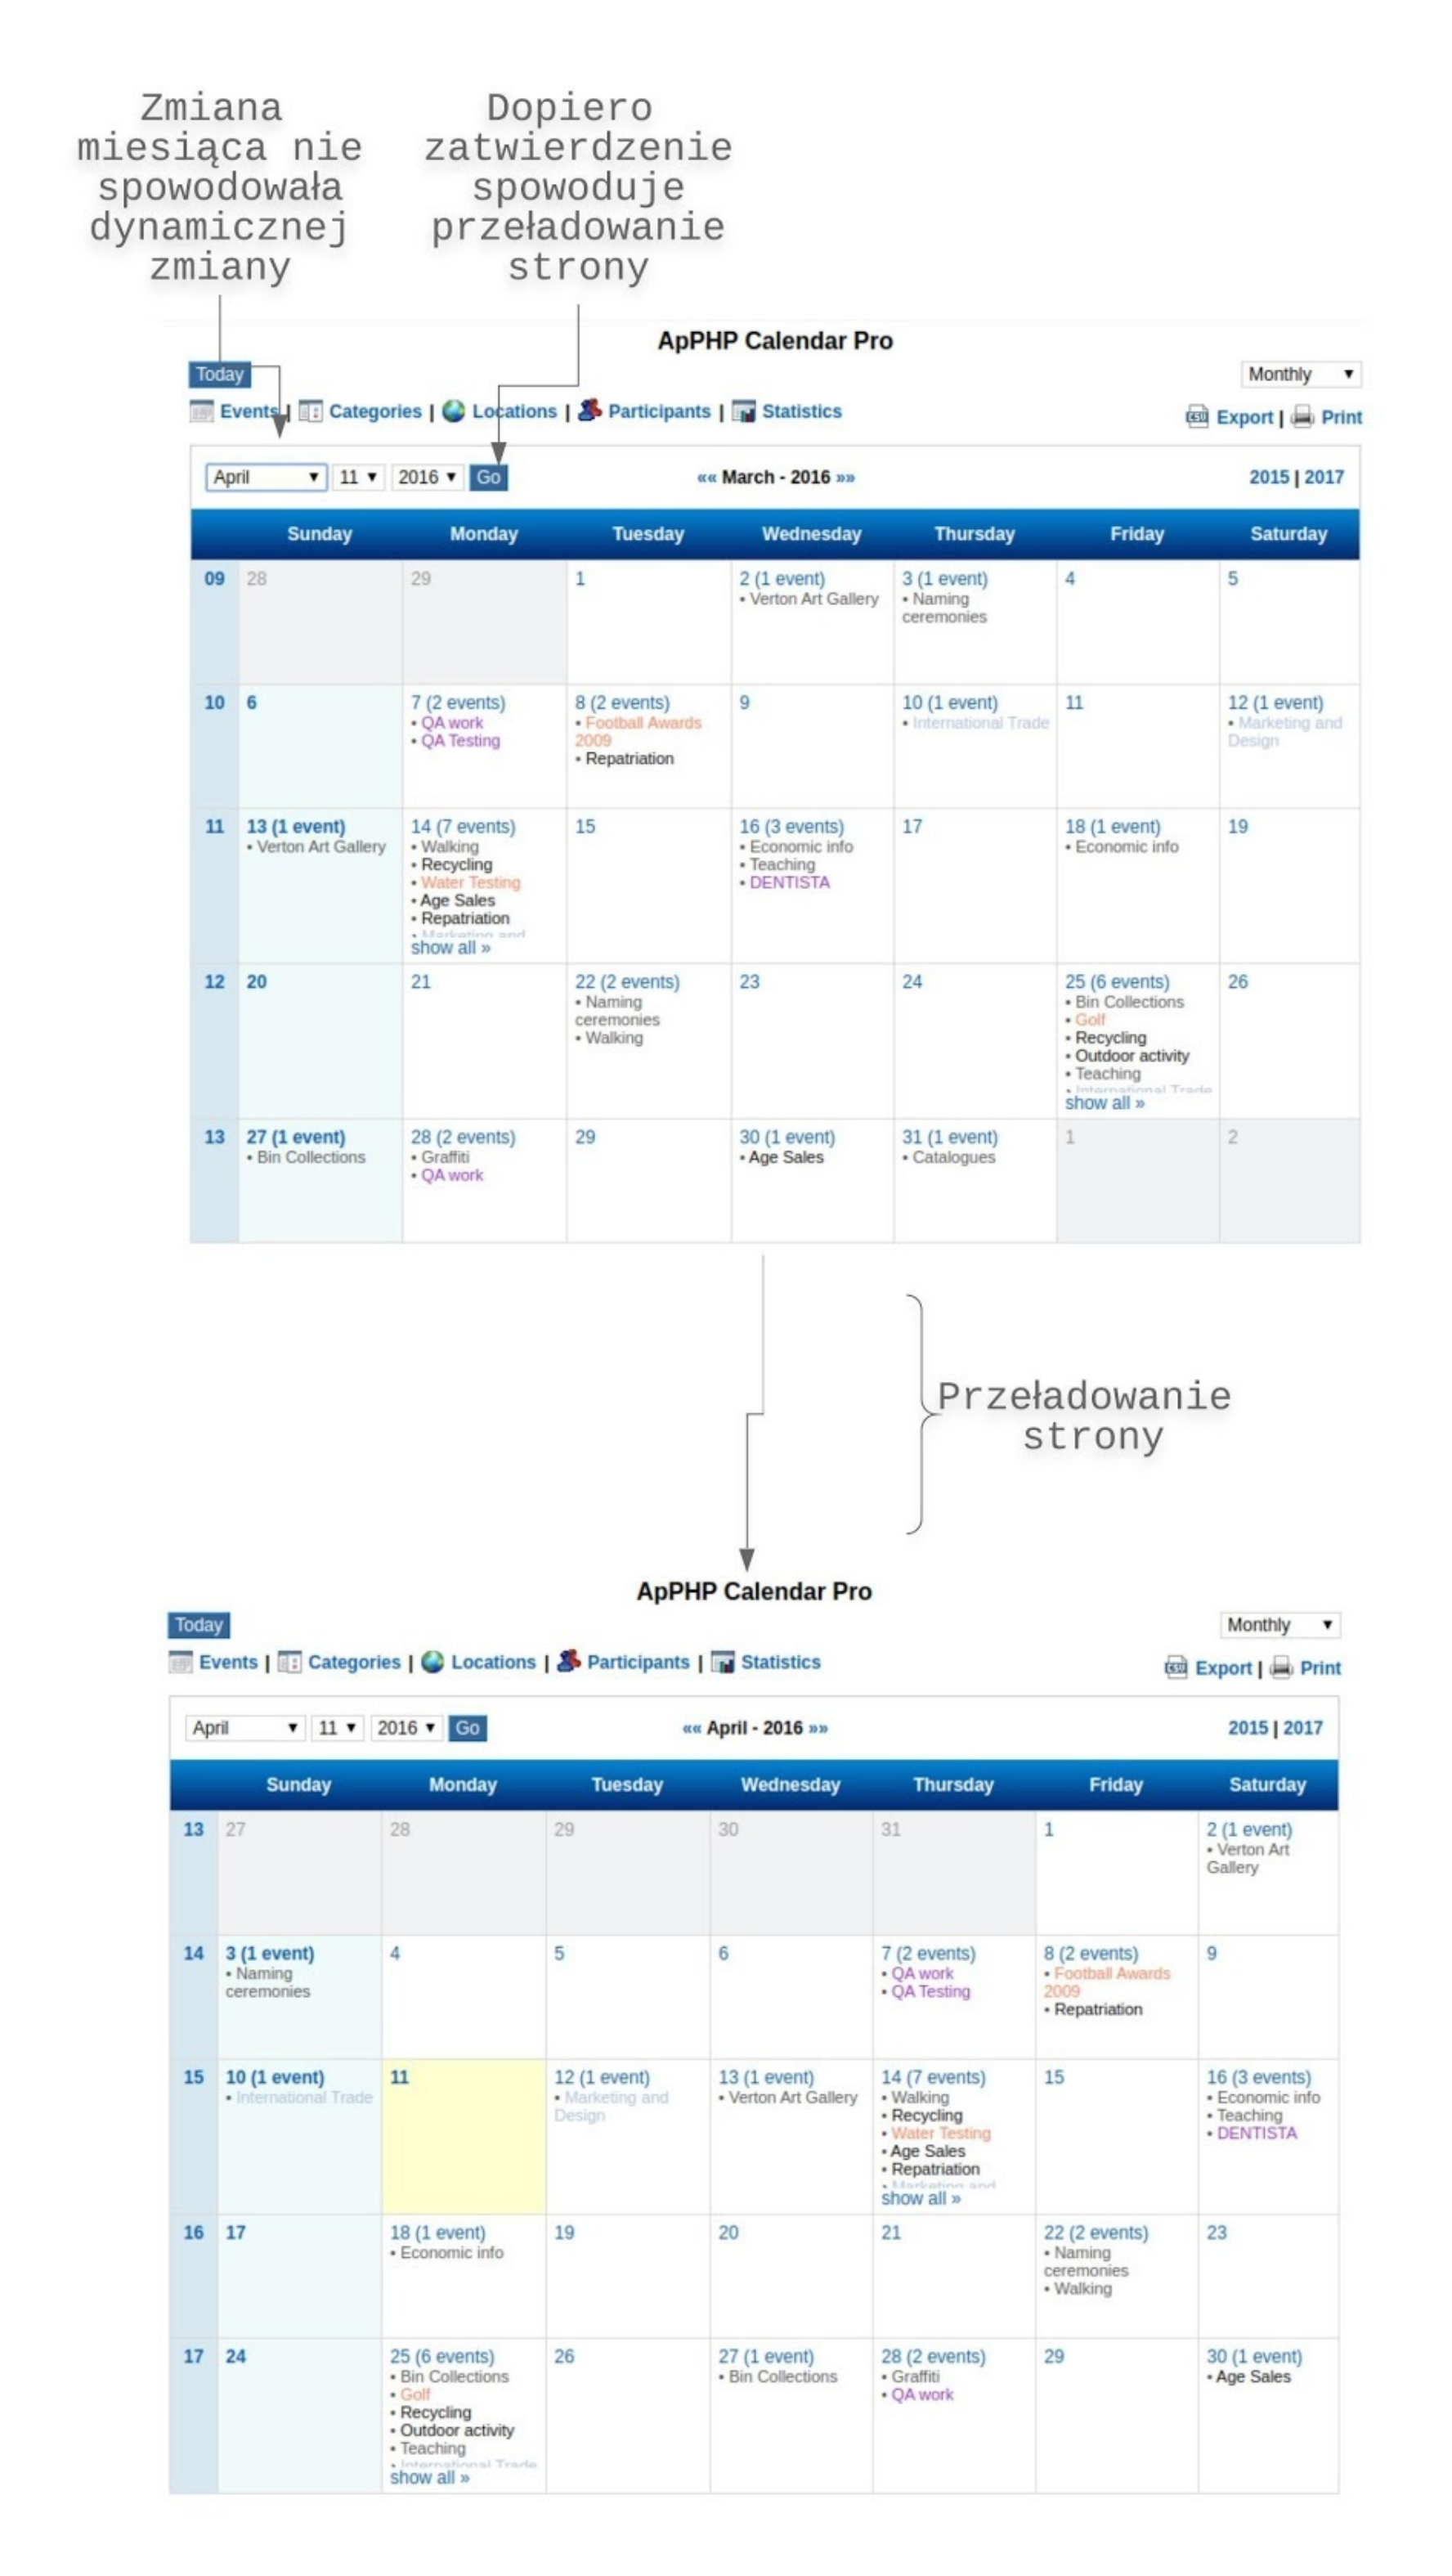
\includegraphics[width=13cm]{rysunek_18.png}
    \caption{Ilustracja mechanizmu działania strony statycznej na przykładzie aplikacji kalendarza przy użyciu języka PHP \cite{app-php-calendar-pro}}
    \label{fig:rysunek_18}
\end{figure}

Teraz, z punktu badawczego chcemy ustalić ile trwała cała akcja. Prosimy nasz automat o naciśnięcie przycisku.
Poszukujemy odpowiedzi na pytanie, ile czasu upłynie, od momentu naciśnięcia przycisku do momentu wyrenderowania nowej treści. Przeanalizujmy więc cały proces ukazany na rysunku \ref{fig:rysunek_19}.

\begin{figure}[htbp]
    \centering
    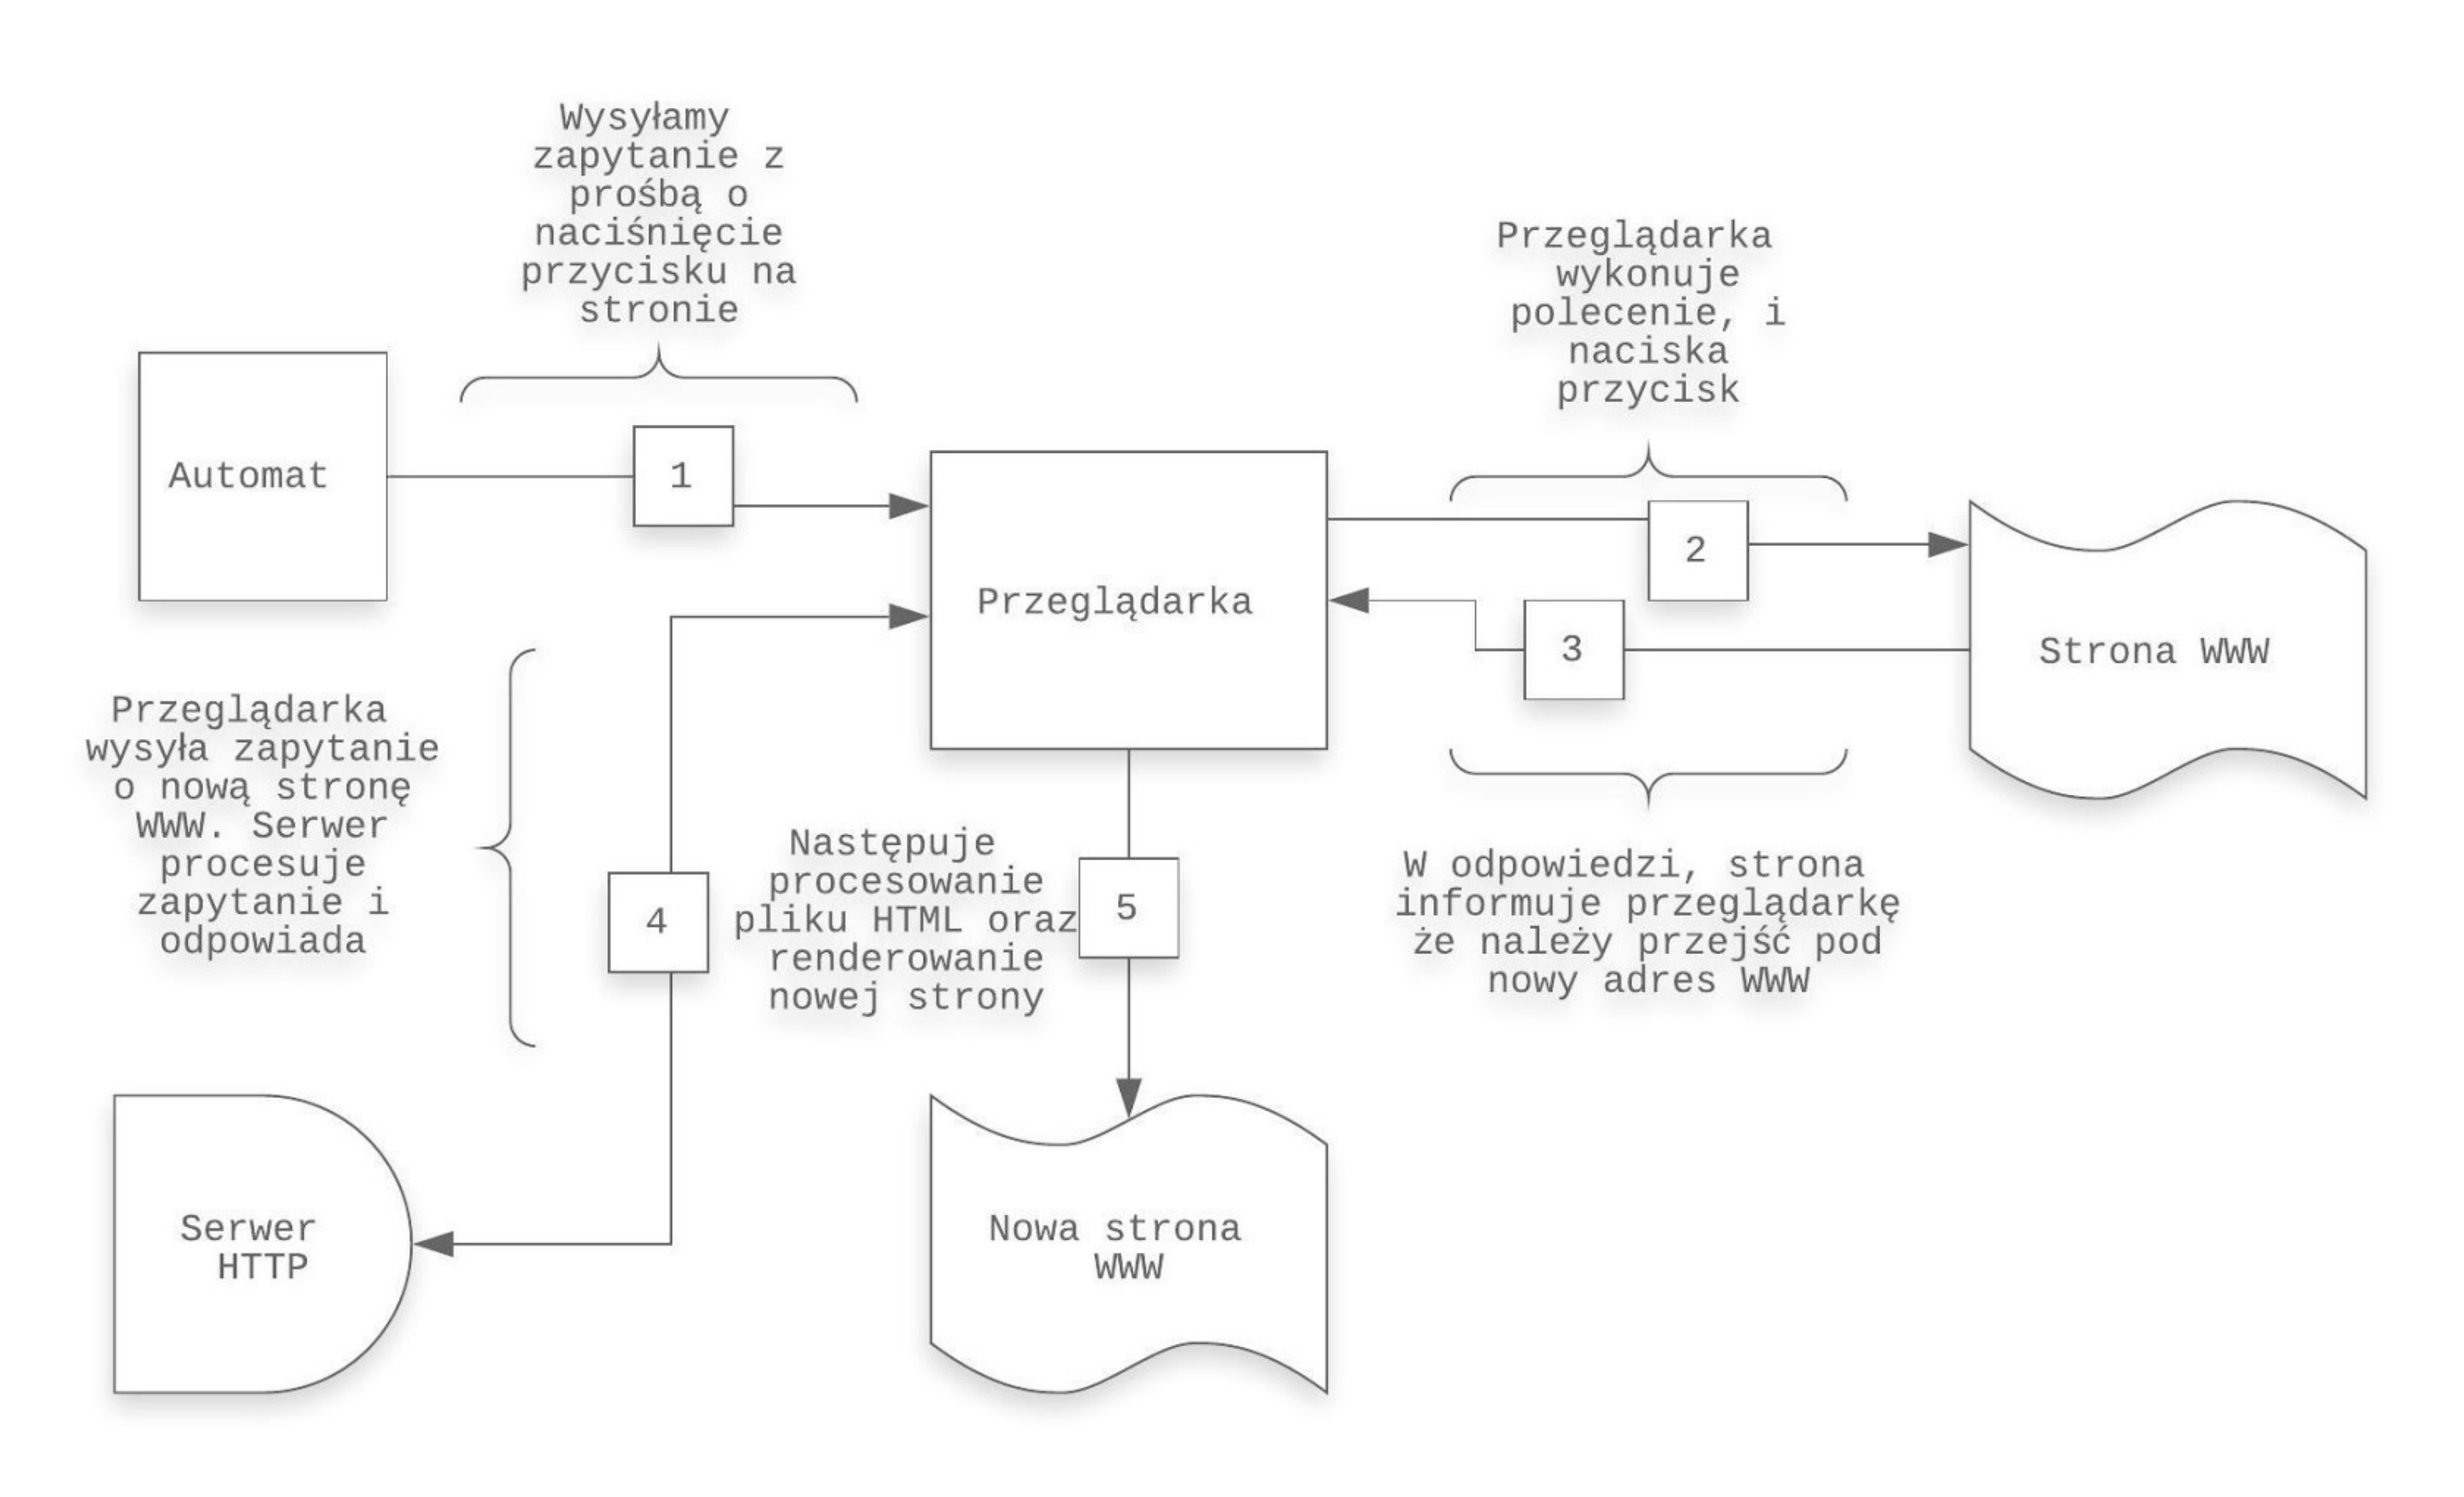
\includegraphics[width=\textwidth]{rysunek_19.png}
    \caption{Grafika przedstawiająca proces przeładowania strony statycznej}
    \label{fig:rysunek_19}
\end{figure}

Z punktu widzenia automatu do testów end-to-end, cały proces, o ile skomplikowany ma jasno zdefiniowany koniec.
Końcem całego procesu jest przeładowanie strony przez przeglądarkę oraz wyrenderowanie treści.
Przeglądarka posiada wbudowane w swoje API szereg zdarzeń które deweloperzy, a więc także automaty, mogą nasłuchiwać.
W naszym przypadku, będzie to First Meaningful Paint \cite{rail-model} które oznacza, kiedy pierwsza treść dostępna dla użytkownika zostaje w pełni namalowana.
Kolejność zdarzeń ukazano na rysunku \ref{fig:rysunek_20}.

\begin{figure}[htbp]
    \centering
    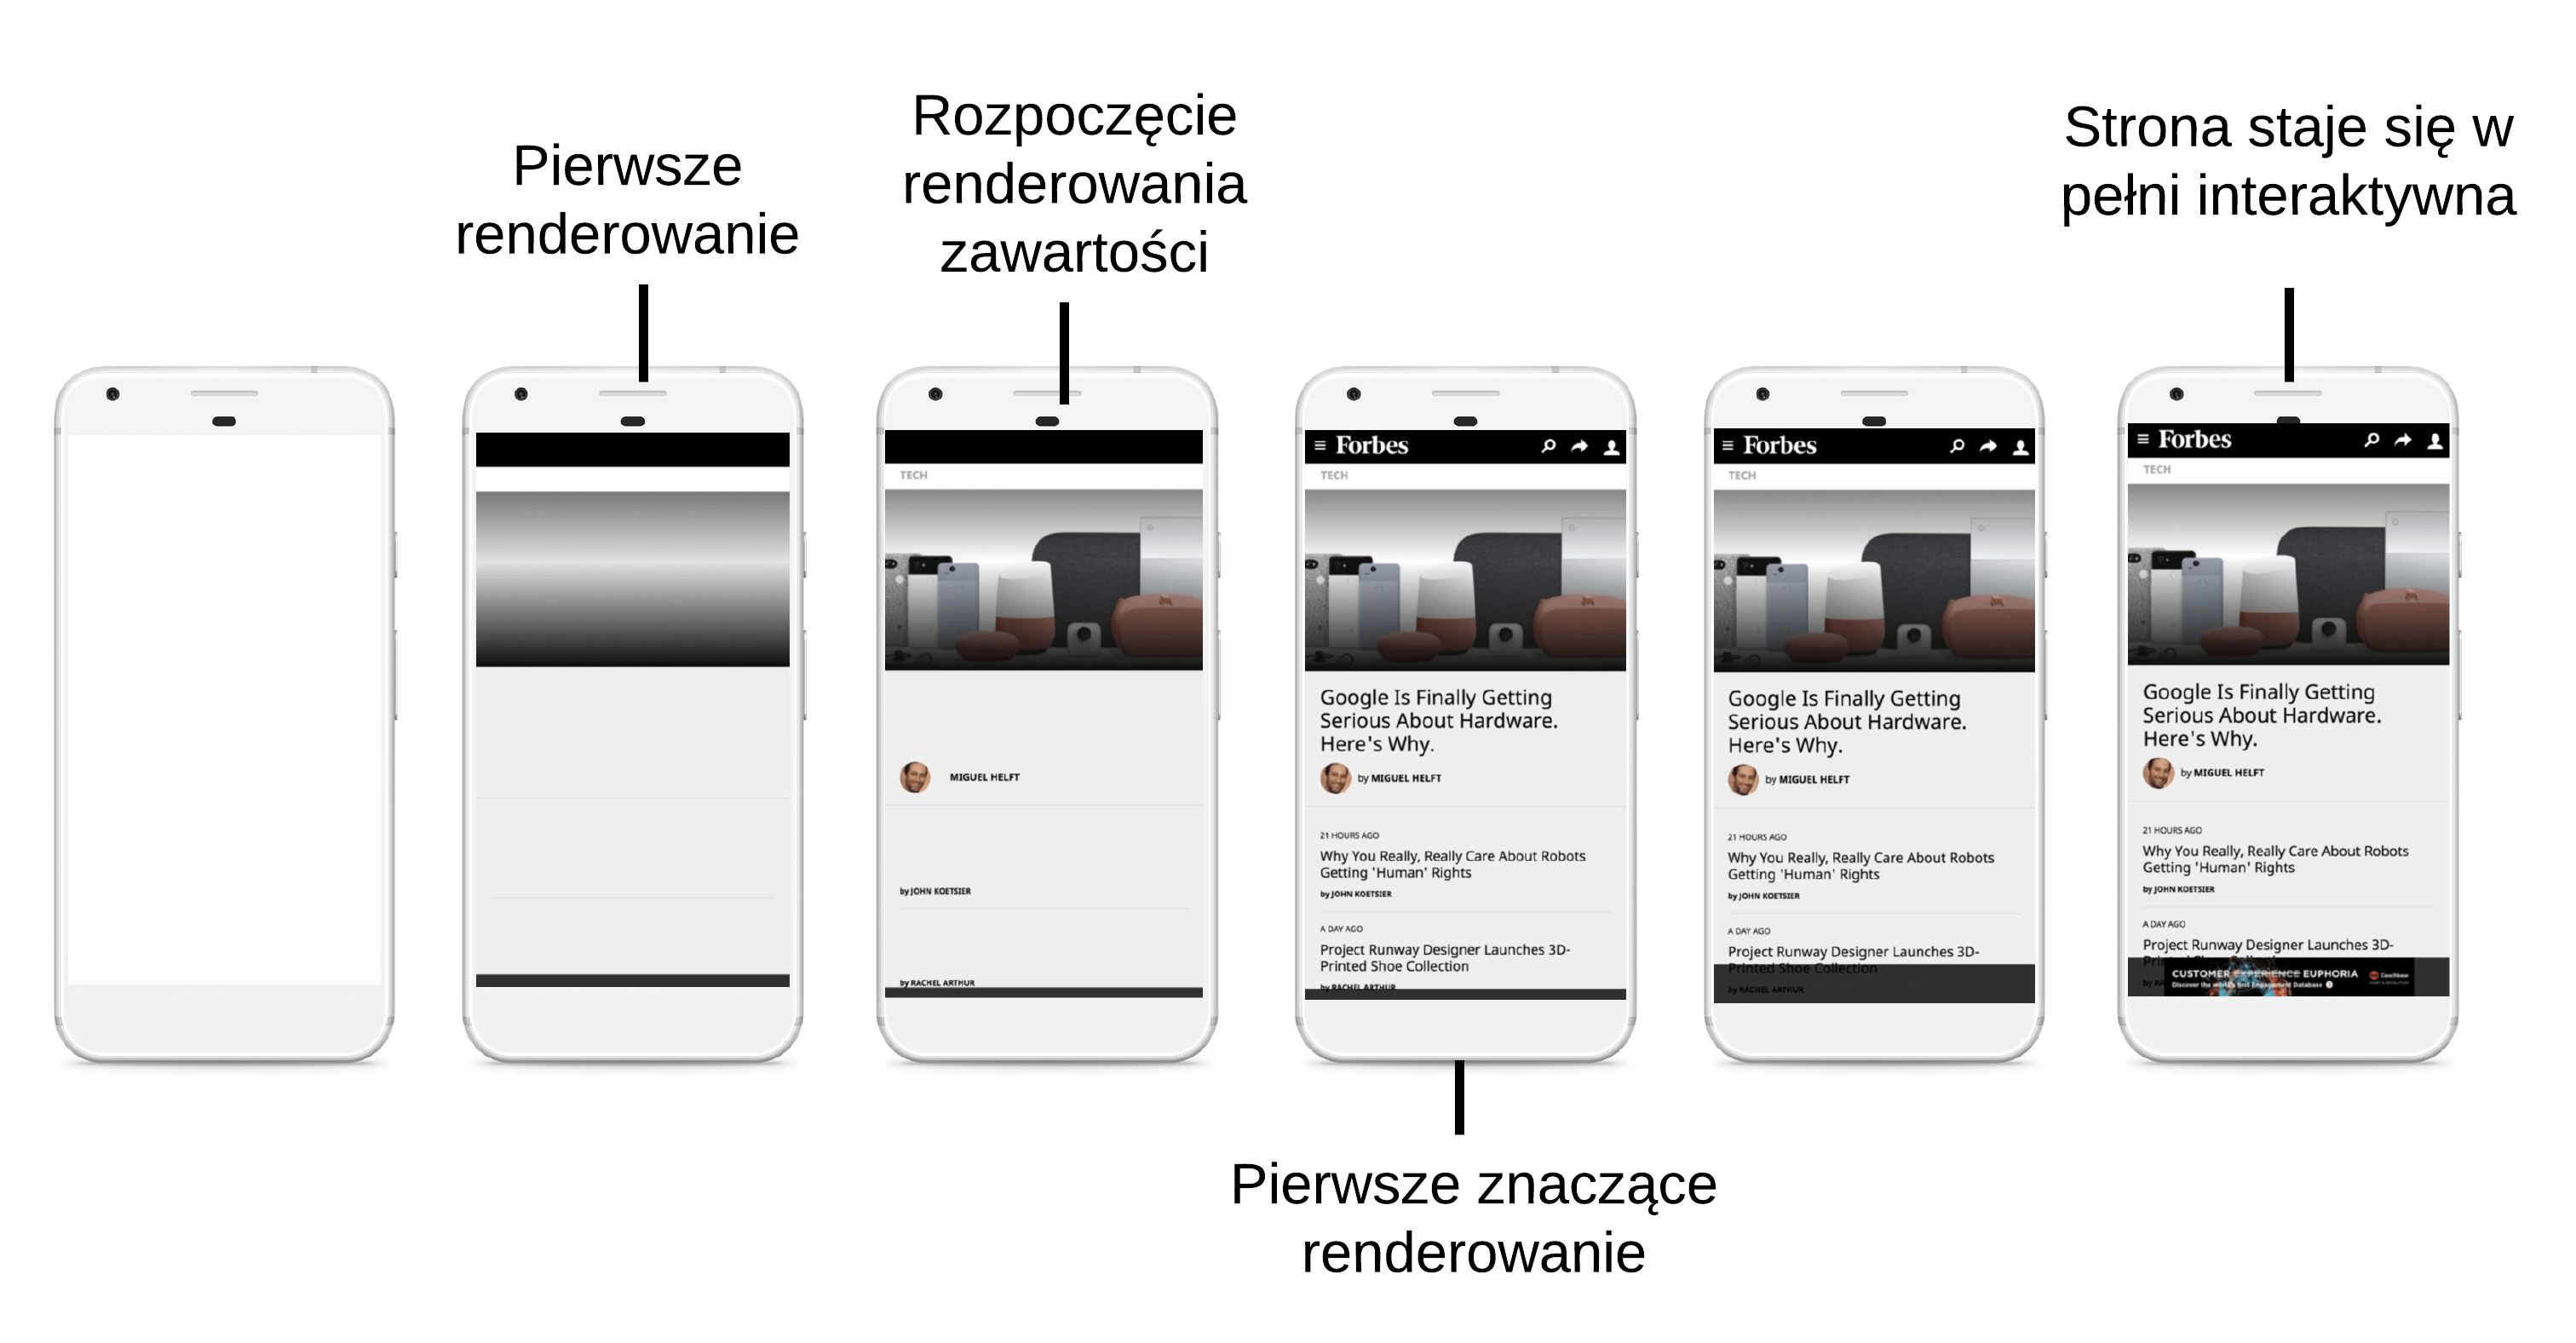
\includegraphics[width=\textwidth]{rysunek_20.png}
    \caption{Ilustracja procesu ładowania aplikacji oraz zdarzenia rejestrowane przez przeglądarkę \cite{rail-model}}
    \label{fig:rysunek_20}
\end{figure}

Tak więc widzimy, że w procesie interakcji ze stroną statyczną, czas jaki będzie potrzebny na przeładowanie strony to nie tylko czas kliknięcia na przycisk, ale także:
\begin{itemize}
    \item Czas potrzebny na wysłanie zapytania z automatu do przeglądarki z żądaniem wykonania akcji
    \item Czas, jaki przeglądarka potrzebuje na naciśnięcie przycisku
    \item Czas wysłania zapytania do serwera
    \item Czas, jaki serwer WWW potrzebuje na skonstruowanie odpowiedzi z plikiem HTML dla przeglądarki. Dla nietrywialnych stron, może to stanowić większą część czasu całej akcji
    Przykładem takiego mechanizmu są strony napisane przy użyciu Ruby on Rails gdzie do skonstruowania nowej strony HTML
    należy przekształcić wzorce HAML \cite{ruby} na plik HTML, często po drodze wykonując zapytanie do bazy (może wielu baz?) danych
    \item Czas ponownego przesłania treści nowej strony do przeglądarki
    \item Czas procesowania nowego pliku HTML oraz wyrenderowanie nowej strony
\end{itemize}

Możemy wyróżnić 3 bazowe serwisy stanowiące rdzeń całej operacji.
Jest to przeglądarka, serwer HTTP oraz automat.
W zależności od maszyny jaką dysponujemy, przeprowadzając takie badanie, wpływ na czas każdej z operacji pośrednich ma to co dzieje się aktualnie na komputerze.
I tak, wpływ będzie miał na przykład program antywirusowy działający w tle, lub inna przeglądarka otworzona obok.
Oczywiście im więcej rdzeni \cite{threads} posiada nasz procesor, tym mniejszy wpływ na badanie będą miały programy współdziałające.
Z tego względu podczas badania należy wykonać nie tylko pojedynczy pomiar, ale pomiary należy wykonywać wielokrotnie tak, aby wyliczyć na przykład
odchylenie standardowe czasów od uśrednionej wartości.

Mając już wiedzę, jak wygląda akcja naciśnięcia przycisku na stronie statycznej, możemy porównać ją do strony aplikacji SPA.
Jako przykład mamy podobny kalendarz jak na stronie statycznej, tym razem z użyciem dynamicznej biblioteki JavaScript.
Na rysunku \ref{fig:rysunek_21} przedstawiono zmianę daty aplikacji dynamicznej z punktu widzenia użytkownika.
Na rysunku \ref{fig:rysunek_22} przedstawiono rozpisaną kolejność zdarzeń z punktu widzenia komputera.

\begin{figure}[htbp]
    \centering
    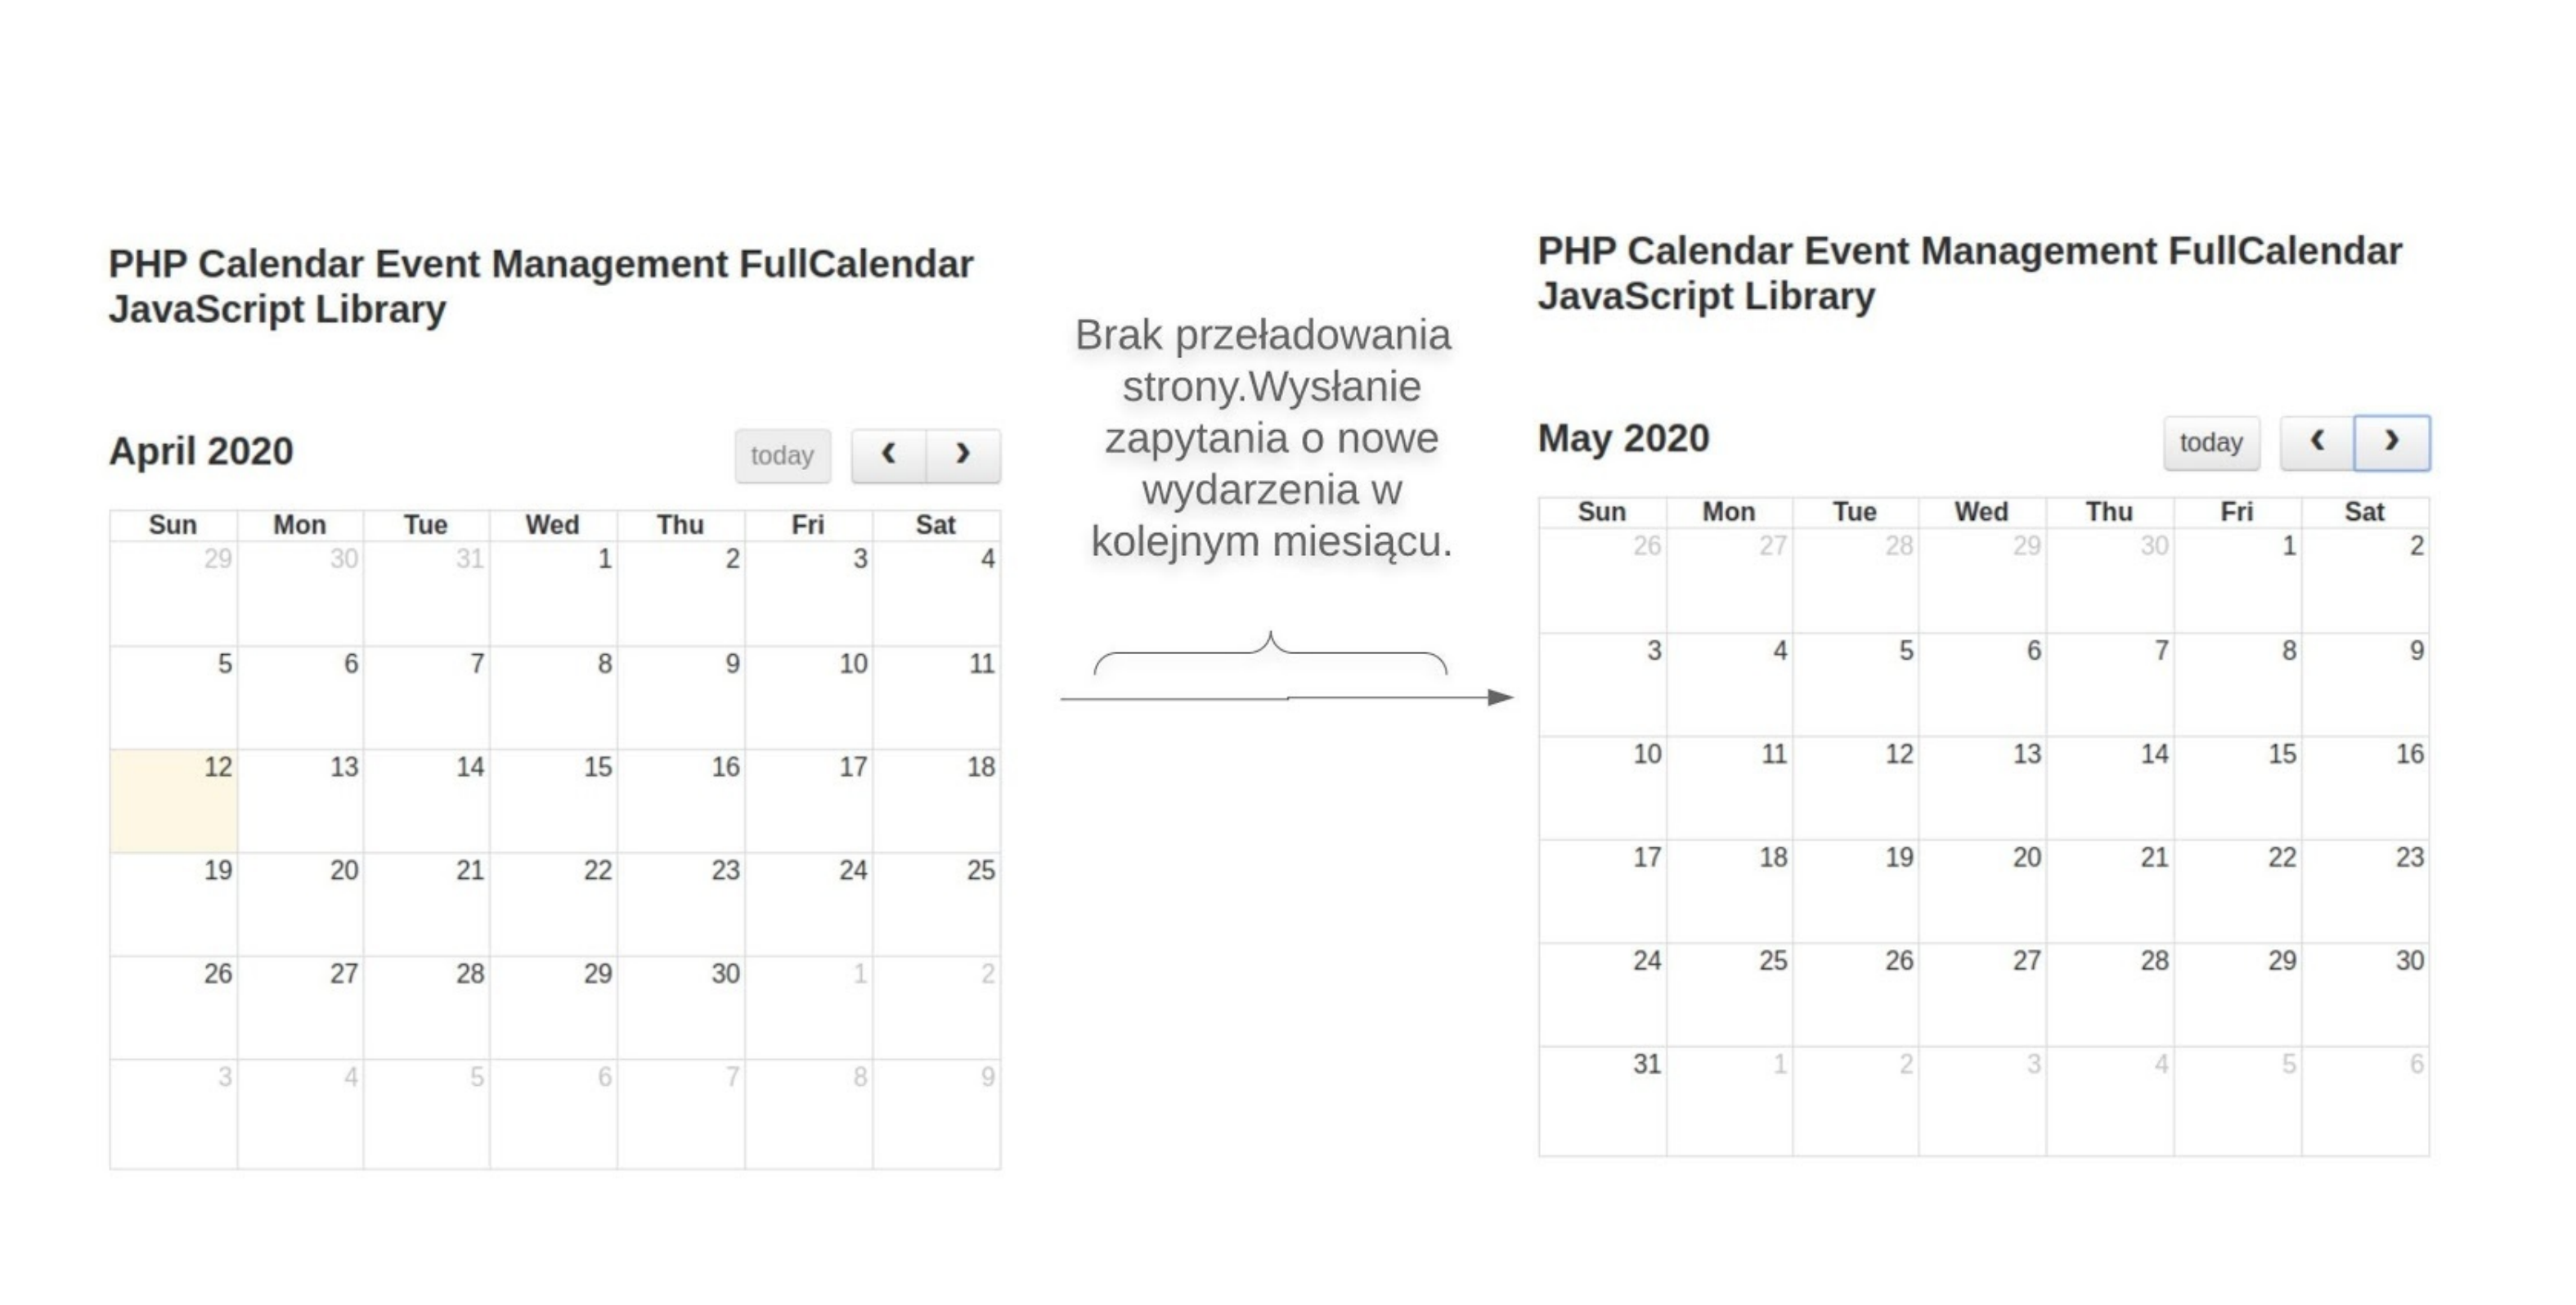
\includegraphics[width=\textwidth]{rysunek_21.png}
    \caption{Ilustracja mechanizmu zmiany daty w przypadku aplikacji dynamicznej z punktu widzenia użytkownika \cite{php-dynamic-app}}
    \label{fig:rysunek_21}
\end{figure}

\begin{figure}[htbp]
    \centering
    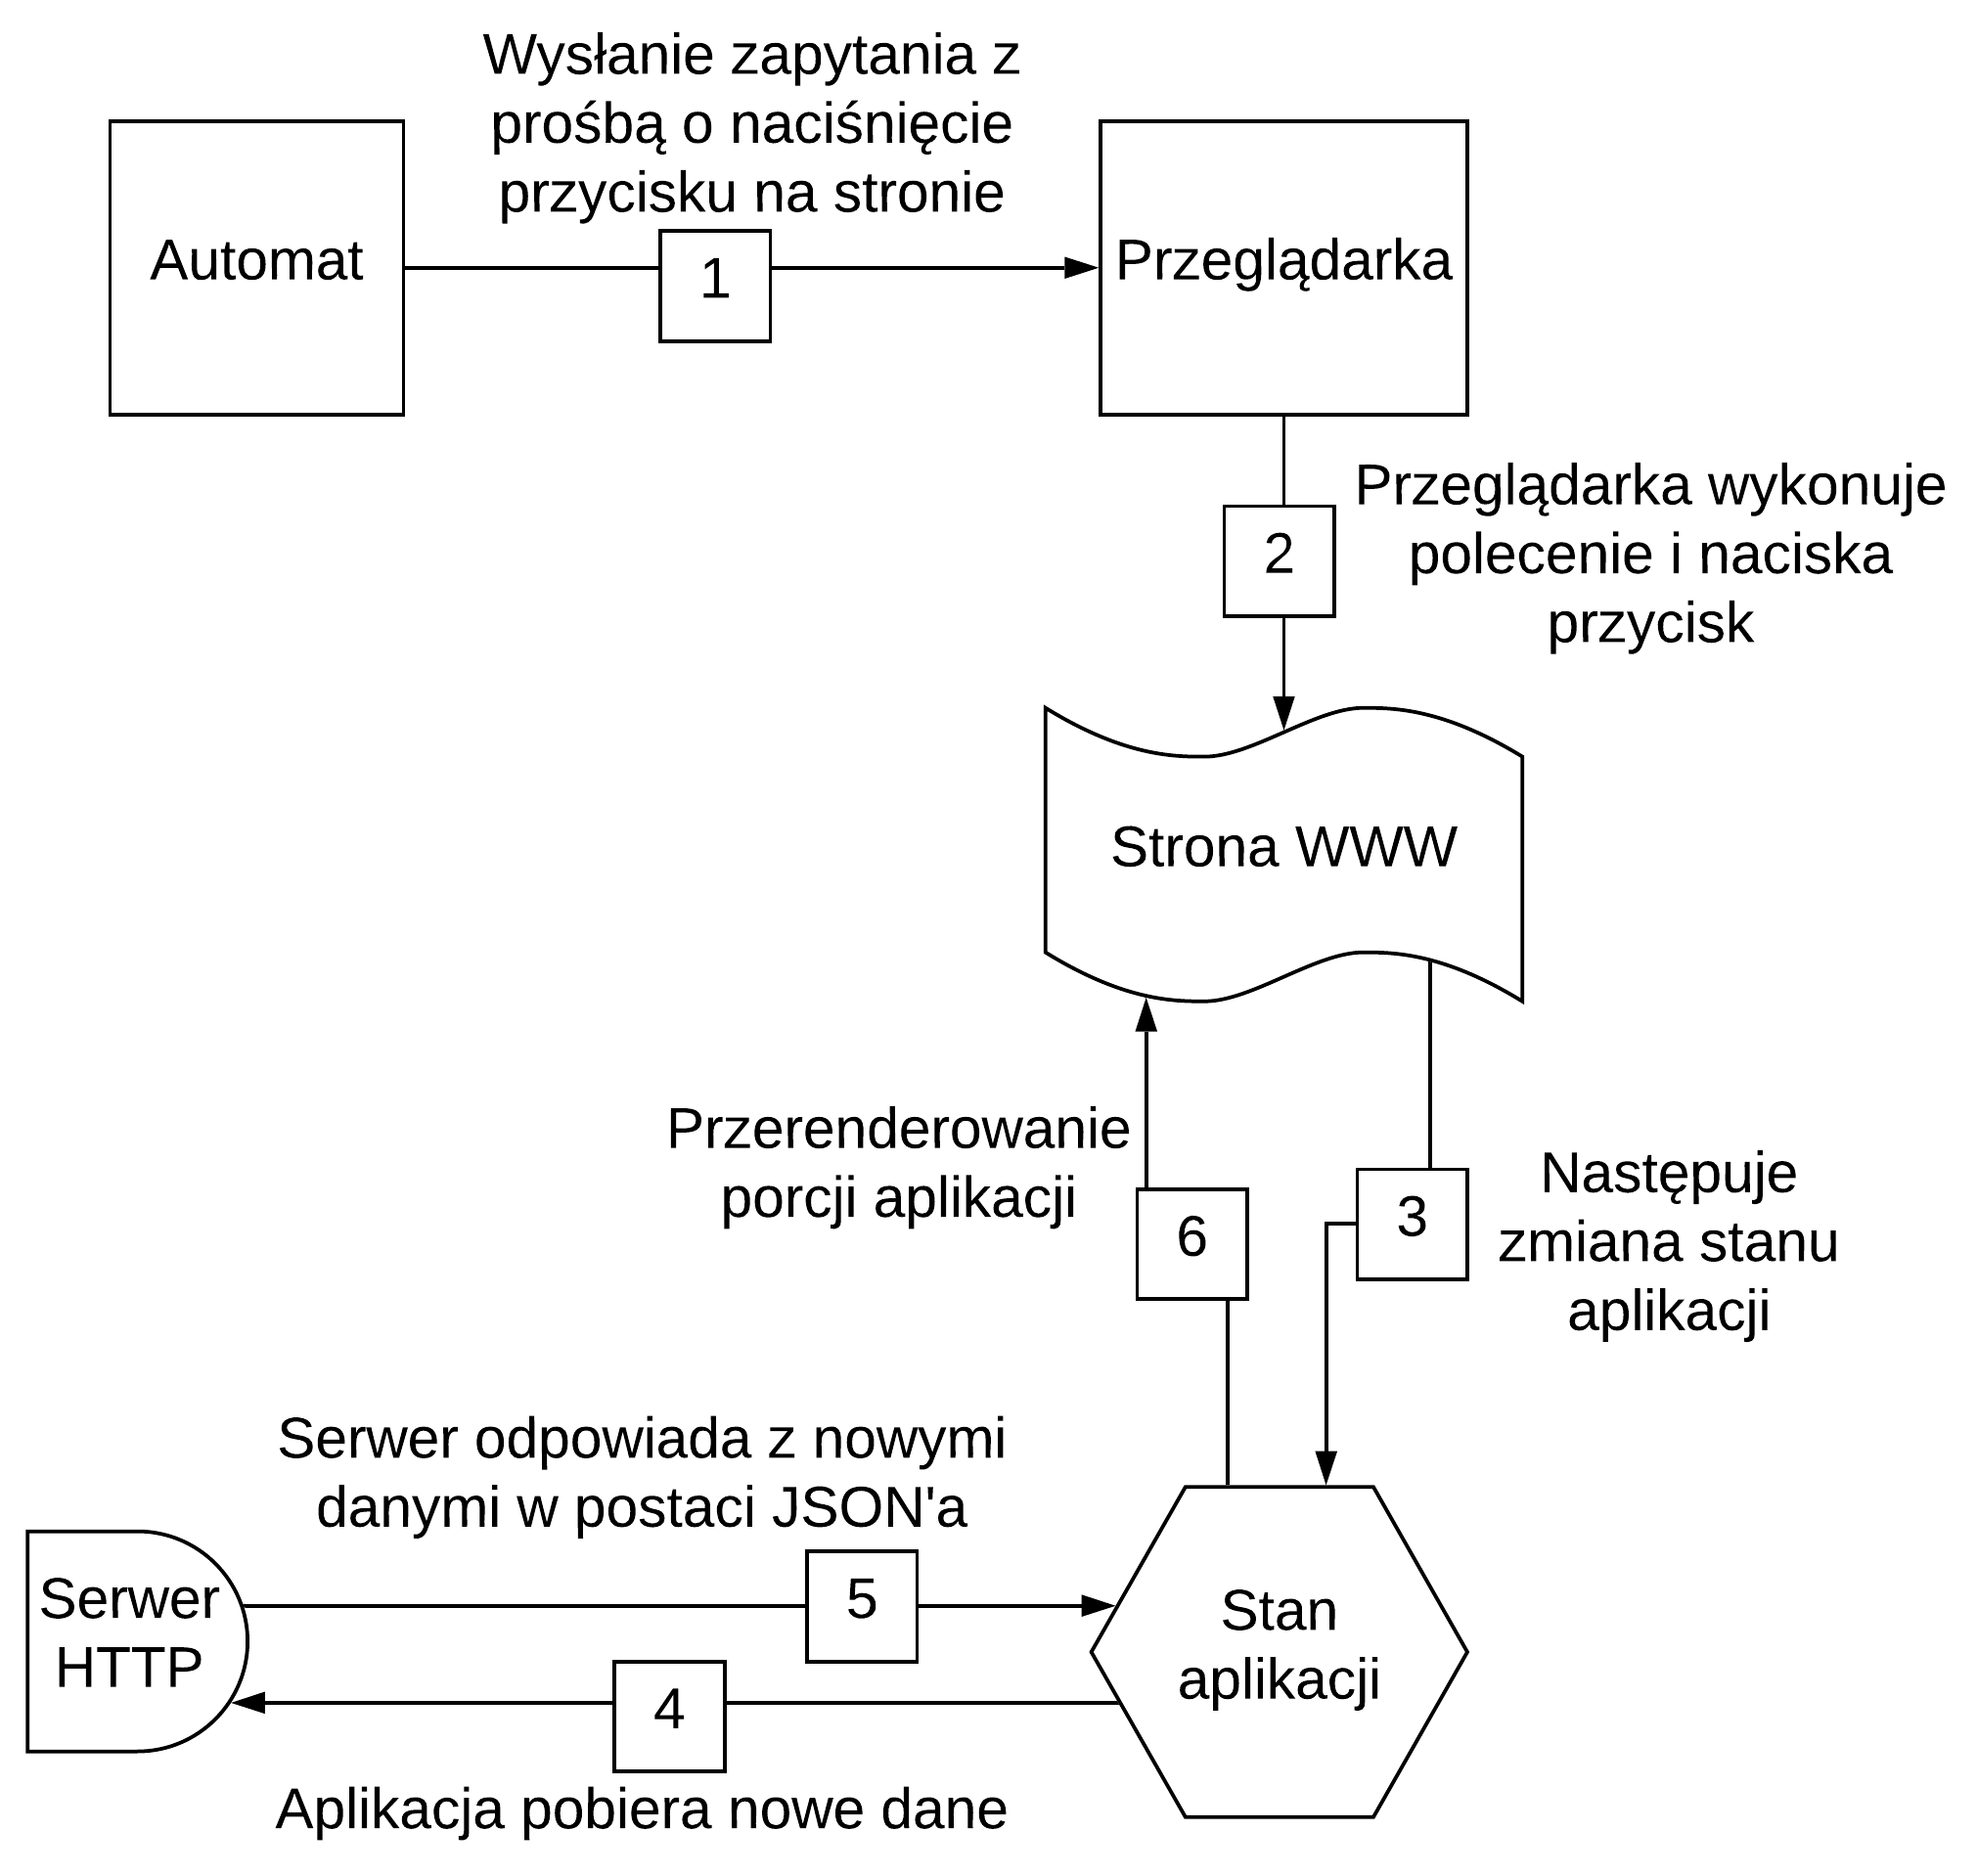
\includegraphics[width=\textwidth]{rysunek_22.png}
    \caption{Ilustracja przedstawiająca proces zmiany treści strony w przypadku aplikacji dynamicznej z punktu widzenia komputera}
    \label{fig:rysunek_22}
\end{figure}

Początek procesu jest taki sam, lecz zarządca stanu aplikacji widząc prośbę o zmianę miesiąca, wysyła zapytanie do serwera.
Serwer przygotuje odpowiedź ale zamiast strony HTML, serwer odpowie ze strukturą danych typu JSON.
Następnie zarządca stanu zmieni stan i poprosi nasz framework o prze renderowanie strony.
Teraz, z punktu widzenia automatu, nie ma tutaj jednoznacznego punktu końca całej operacji.
Tak jak na stronie statycznej mogliśmy oczekiwać na przeładowanie strony oraz zdarzenie First Meaningful Paint,
tak w tym przypadku nie istnieje żadne API pozwalające na precyzyjne określenie czy cała akcja została zakończona.
Jest to bardzo kosztowny problem z którym branża informatyczna zmaga się od bardzo dawna. Wiodącym jak na razie rozwiązaniem tego problemu,
które i tak nie jest idealne jest sposób testowania narzędzie Cypress.io.

\begin{itemize}
    \item Sprawdza, czy w przeglądarce istnieją nierozwiązane zapytania HTTP
    \item Sprawdza, czy aktualnie renderowana jest jakaś nowa zawartość
    \item Wykonuje serię screenshotów i porównuje, czy zawartość zmienia się w czasie
    \item Periodycznie próbkuje, czy zawartość DOM została już zmieniona
\end{itemize}

Jednak nawet nowoczesne metody zastosowane w narzędziu Cypress nie są wystarczające aby zapewni, iż nawet poprawnie napisane testy zawsze zakończą się sukcesem.
Zjawisko to nazywamy testami flaky, gdyż ze względu na czynniki zewnętrzne takie jak na przykład test A/B, mimo, iż sama implementacja testu jest poprawna,
nadal może on zakończyć się niepowodzeniem \cite{flaky-cypress}. Ze względu na opisane powyżej problemy, postanowiono zbudować moduł badania strony w oparciu o narzędzie Selenium \cite{selenium}.
Jest to najbardziej dojrzałe narzędzie na rynku, które stanowi bazę całego badania.

Pierwszym krokiem potrzebnym do zbudowania modułu, jest konteneryzacja samego Selenium.
W tym celu, wykorzystam narzędzie docker compose \cite{docker-compose}.
Pozwala ono na uruchomienie wielu obrazów dockera, oraz połączyć je ze sobą na przykład za pomocą zwirtualizowanej sieci \cite{docker-compose-network}.
Bazowym obrazem będzie \emph{selenium/hub:3.141.59-zinc}.
Selenium hub, posiada w sobie selenium driver, jednak naszym zadanie jest podłączenie do niego wybranej przez nas przeglądarki.
Drugim elementem jest sama przeglądarka, w tym celu wykorzystam obraz \emph{selenium/node-chrome:3.141.59-zinc}.
Ostatnim elementem jest skrypt który wykorzystując stworzony serwis Selenium, wyśle on odpowiednie informacje do przeglądarki,
zagreguje dane oraz zachowa je na dyski do dalszego procesowania i analizy. Proces ten zobrazowano na rysunku \ref{fig:rysunek_23}.

\begin{figure}[htbp]
    \centering
    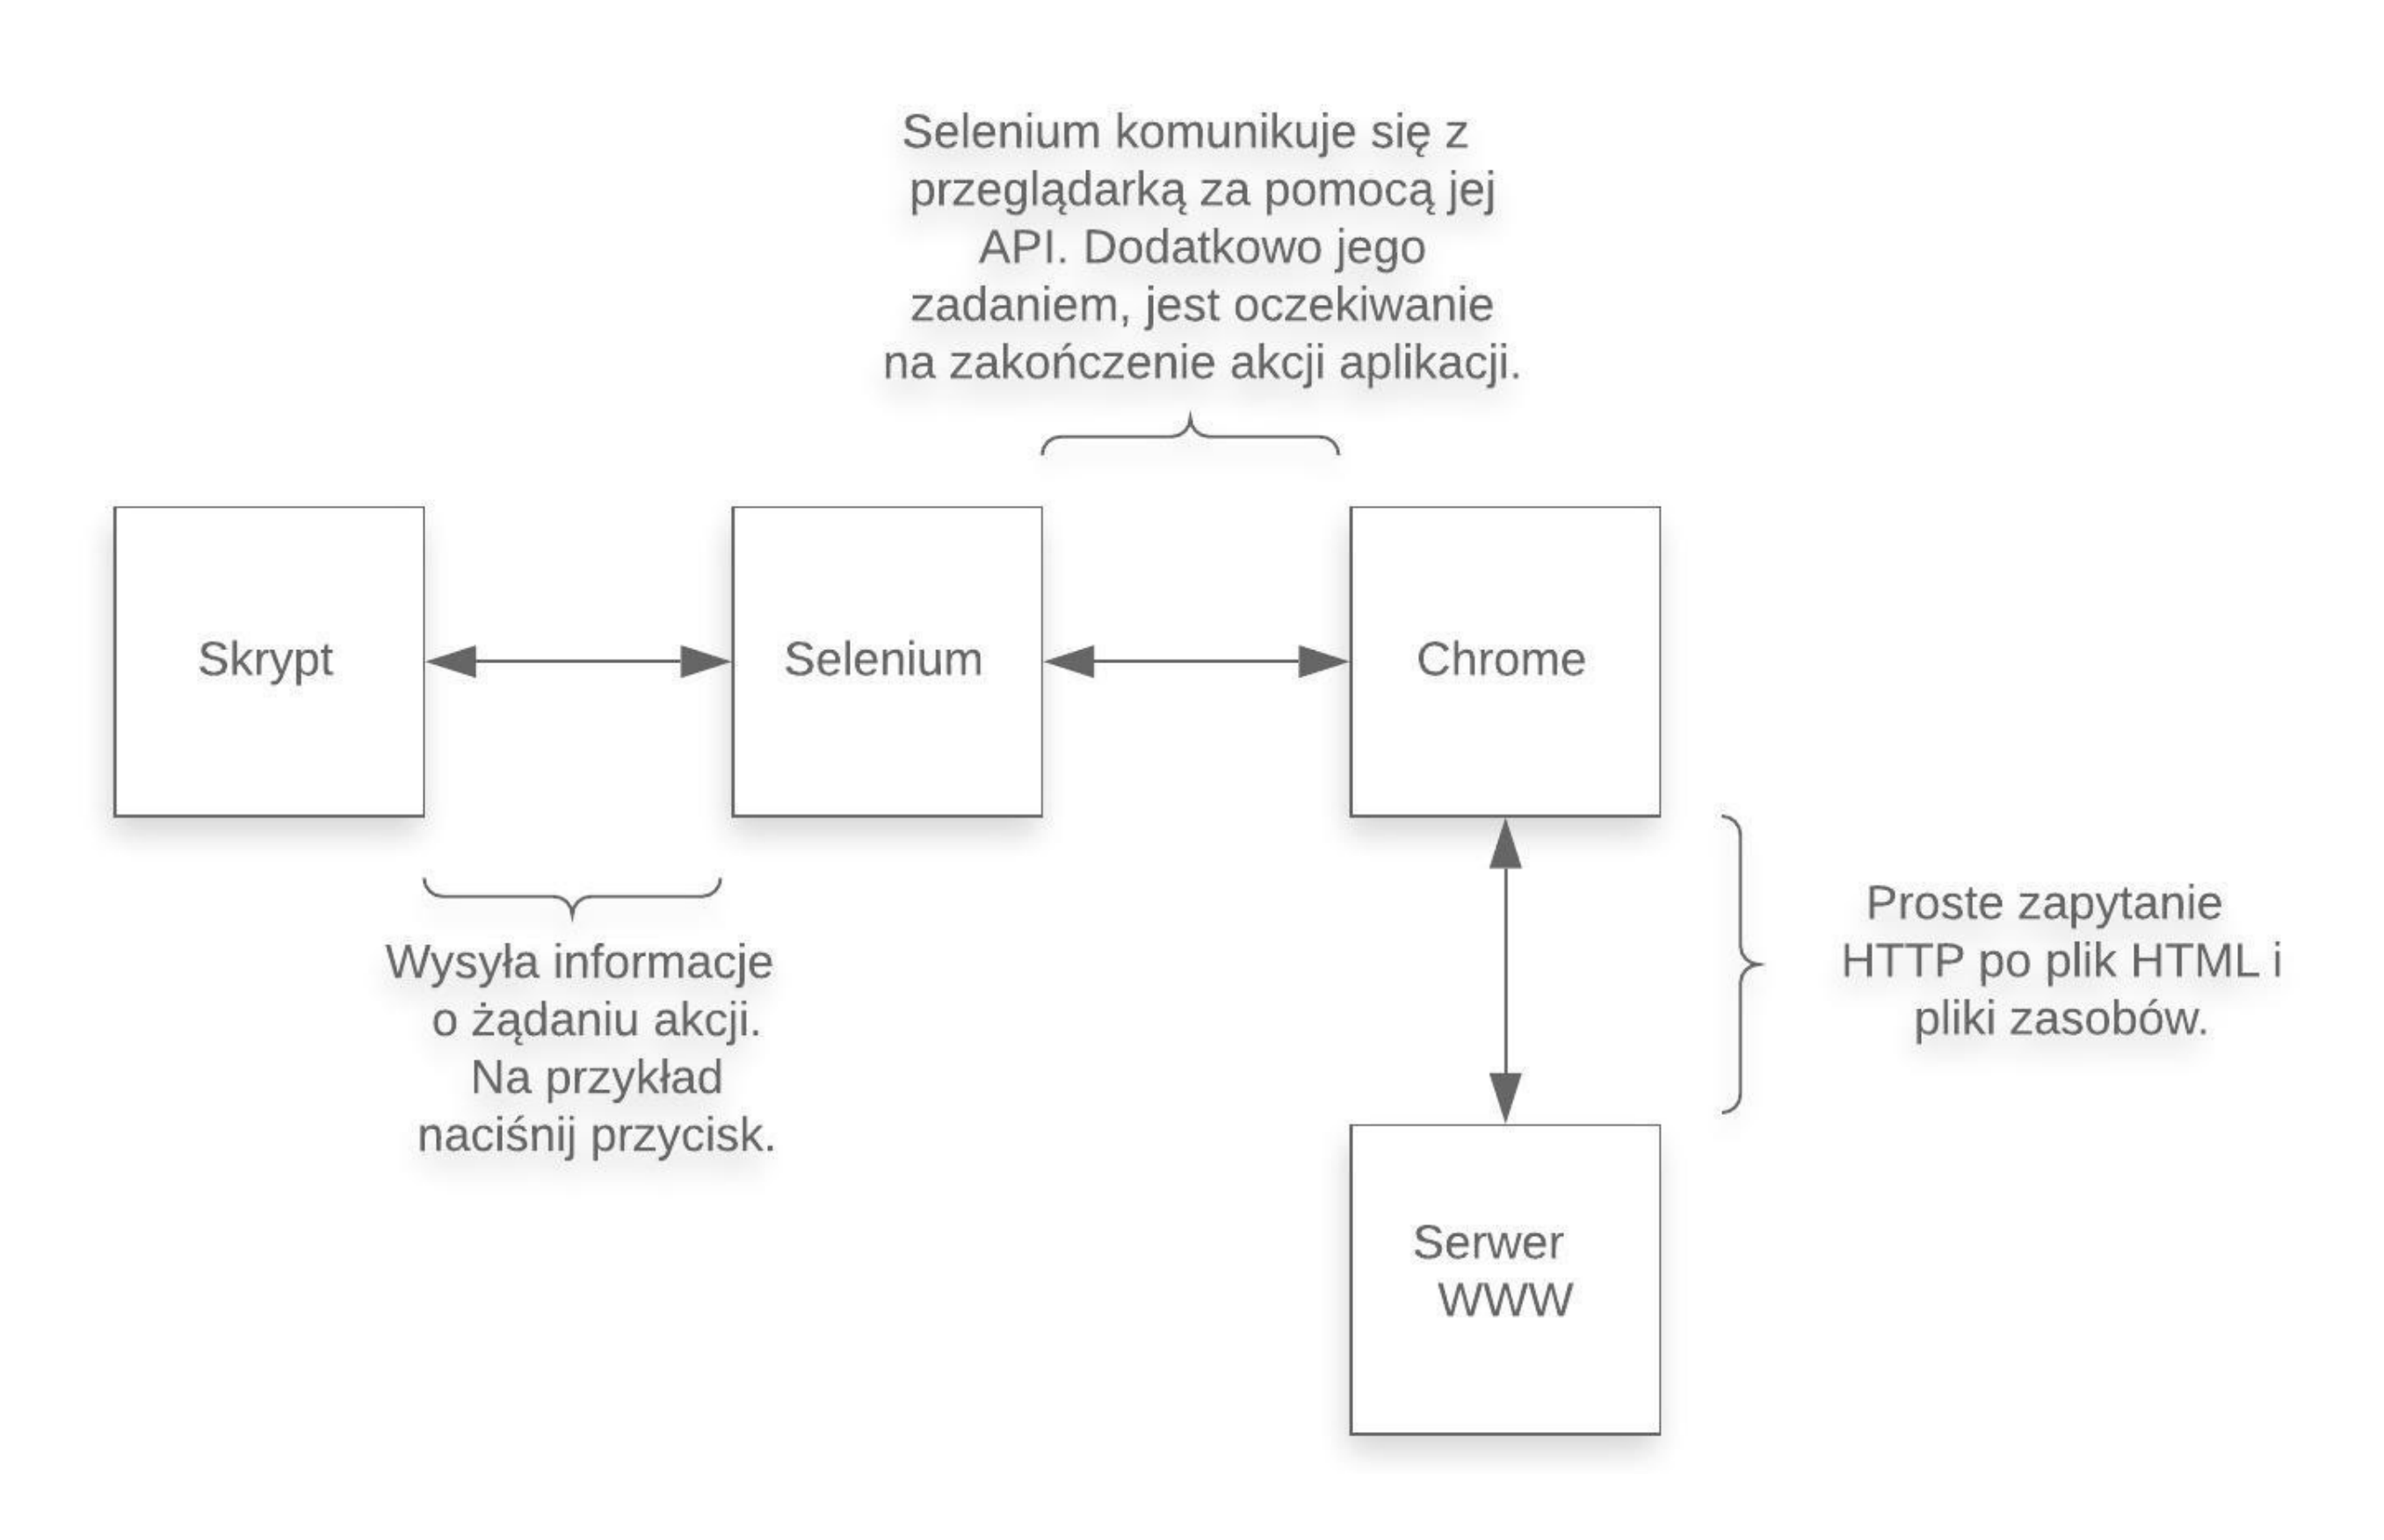
\includegraphics[width=\textwidth]{rysunek_23.png}
    \caption{Ilustracja procesu współpracy pomiędzy Selenium a przeglądarką}
    \label{fig:rysunek_23}
\end{figure}

Skrypt do obsługi Selenium składa się z kilku głównych elementów. Pierwszym z nich jest moduł odpowiadający za oczekiwanie na gotowość systemu.
Z racji, iż Docker compose stara się uruchomić wszystkie obrazy na raz, nie możemy od razu zacząć badania gdyż w pierwszej kolejności,
Selenium hub musi zostać zainicjalizowane, oraz przeglądarka Chrome musi zarejestrować się w systemie.
Z tego powodu stworzono funkcje które pingują Selenium oraz Serwer HTTP w oczekiwaniu na odpowiedź z kodem 200.
Próbujemy połączyć się trzykrotnie z jednosekundowym odstępem czasu. Obydwa mechanizmy pracują asynchronicznie.
Jeżeli którykolwiek z nich po 3 próbach nadal nie będzie mógł się połączyć, cały skrypt zwróci stosowną wiadomość która pomoże nam określić przyczynę problemu.
Próbę uzyskania połączenia zobrazowano na rysunku \ref{fig:rysunek_24}.
Z kolei na rysunku \ref{fig:rysunek_25} widzimy, iż pomimo początkowych problemów z uzyskaniem połączenia, mechanizm zadziałał poprawnie i udało się nawiązać połączenie.

\begin{figure}[htbp]
    \centering
    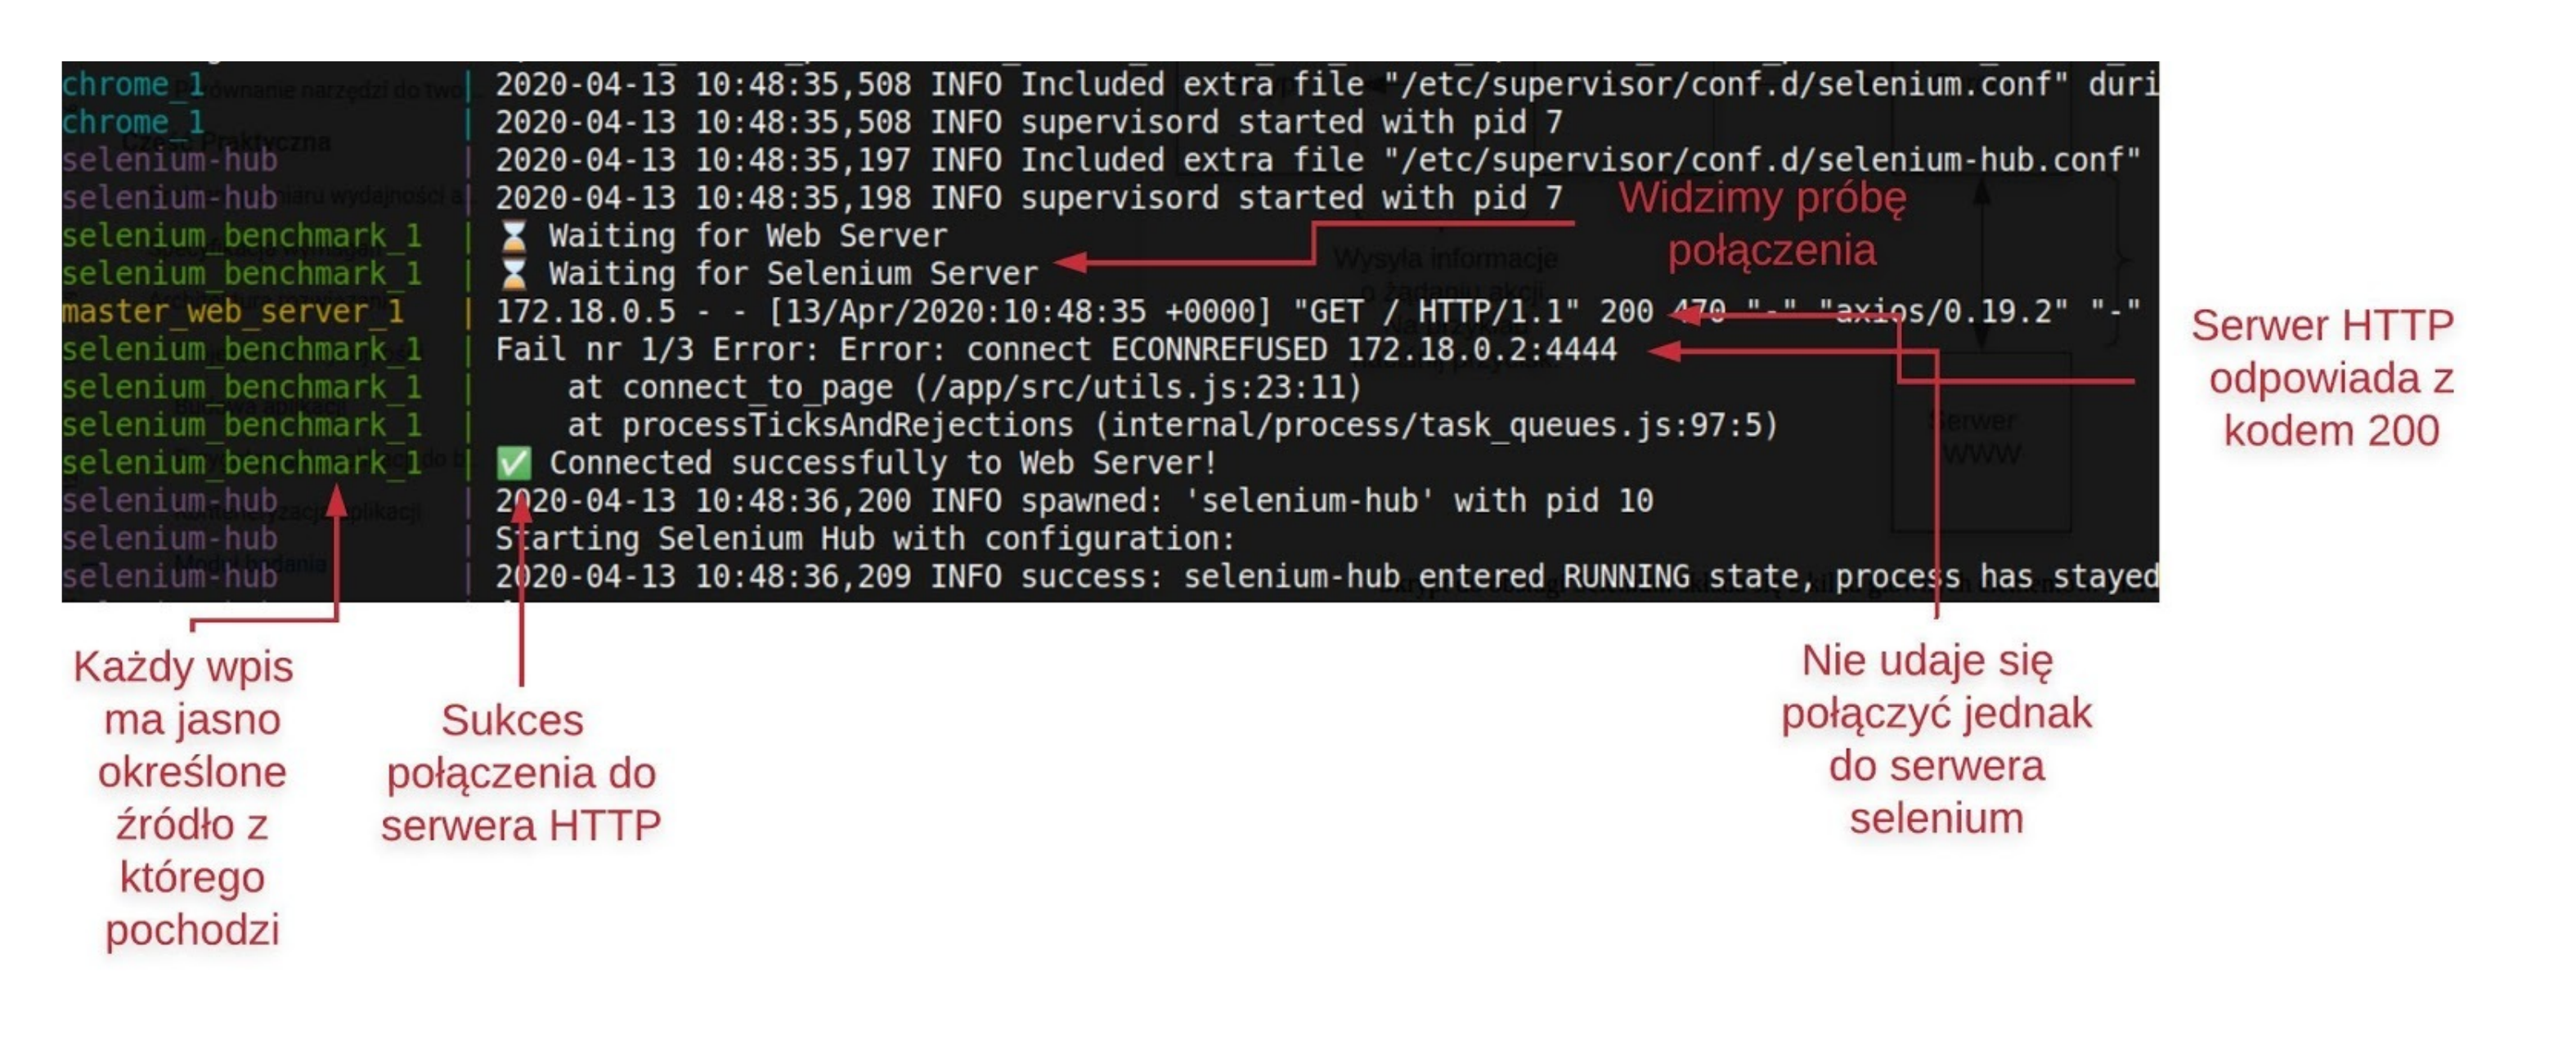
\includegraphics[width=\textwidth]{rysunek_24.png}
    \caption{Wycinek wpisów skryptu przeprowadzającego badanie w środowisku docker-compose. Ilustruje on inicjalizację skryptu oraz mechanizm uzyskiwania połączenia pomiędzy Skryptem - Przeglądarką - Selenium}
    \label{fig:rysunek_24}
\end{figure}

\begin{figure}[htbp]
    \centering
    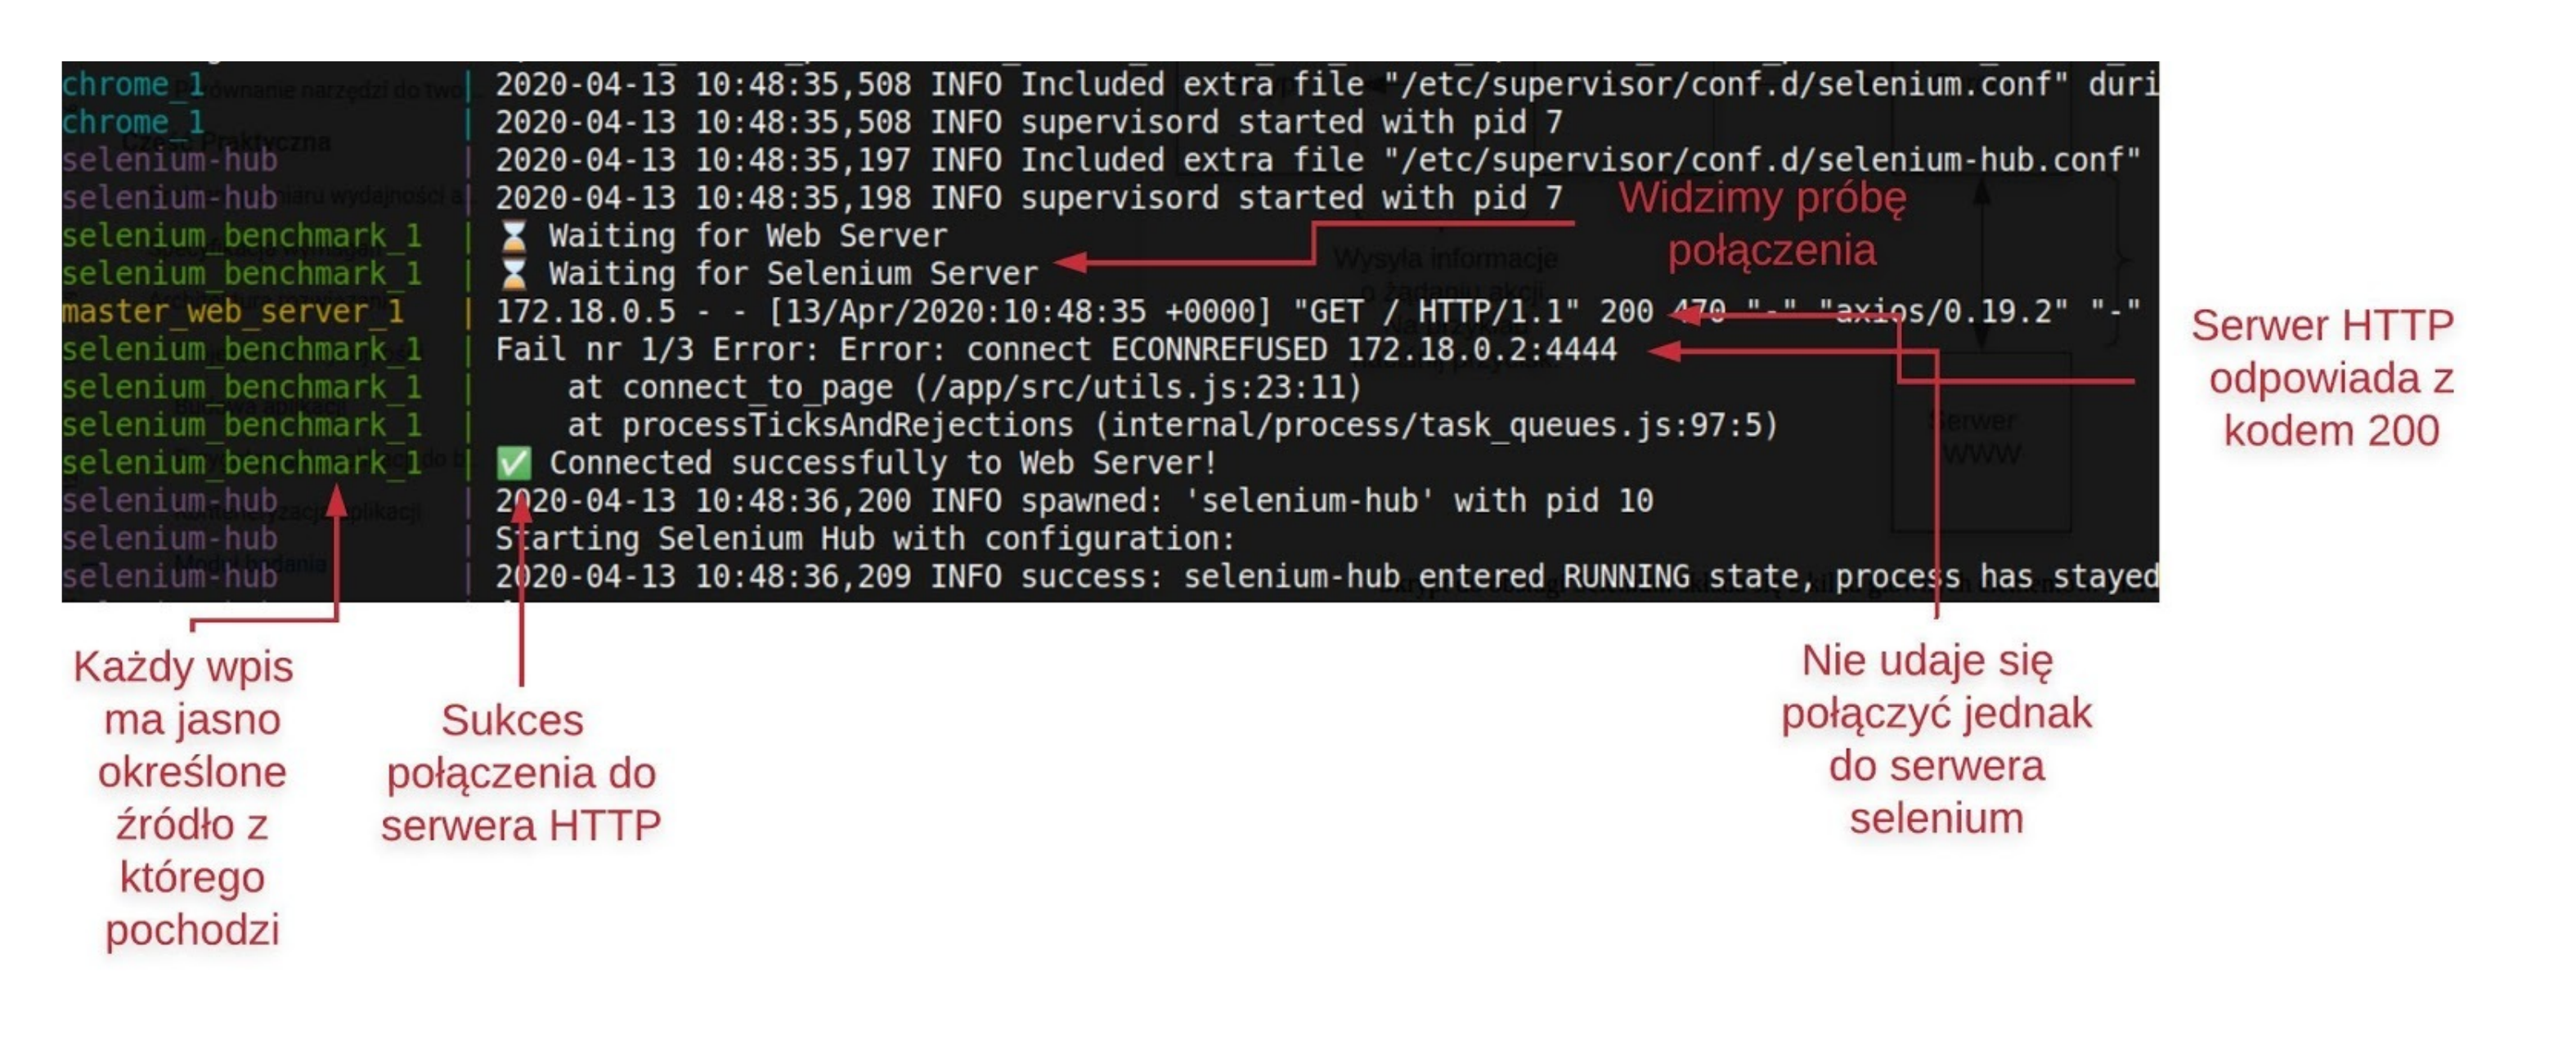
\includegraphics[width=\textwidth]{rysunek_25.png}
    \caption{Wycinek skryptu ukazujący uzyskanie połączenia do Selenium pomimo początkowych problemów}
    \label{fig:rysunek_25}
\end{figure}

Następnie łączymy się do serwera WWW. Odczytujemy z niego listę dostępnych aplikacji.
Dzięki temu, nie musimy zmieniać implementacji kodu testu przy dodawaniu kolejnych implementacji lub badań.
Przed każdym badaniem chcemy jak najbardziej odizolować od siebie testy, z tego też powodu wysyłamy komendę przeładowania strony oraz wyczyszczenia pamięci cache
oraz wołamy komendę garbage collection \cite{mozilla-memory}.
Wreszcie, mając już tak przygotowane środowisko oraz połączenie do Selenium możemy przejść do faktycznej implementacji testu badania.

Obsługa testów została zaprojektowana tak, aby można było dodać dowolną ilość testów oraz dowolnie sprecyzować ilość powtórzeń.
Powtórzenia są dla nas istotne gdyż musimy wykonać ten sam test wielokrotnie w celach porównania wyników i analizy różnicy w czasach w poszczególnych obiegach.
Następnie zostanie omówiona struktura badania którą napisano stricte na potrzeby analizy czasów akcji aplikacji w frameworkach aplikacji SPA.
Test ten otwiera stronę WWW, i dla każdej kolejnej funkcji na początku dopisuje 1000 elementów (tak, aby kolejne komendy miały materiał do pracy)
i po zakończeniu testu danej funkcji czyści wszystkie wiersze. W badaniu następują kolejne zdarzenia:

\begin{itemize}
    \item Wykonuje akcje dopisania 1000 elementów na początku listy, i powtarza ją 100 razy
    \item Wykonuje akcje dopisania 1000 elementów na końcu listy, i powtarza ją 100 razy
    \item Wykonuje akcje zamiany wszystkich wartości na liście, i powtarza ją 100 razy
    \item Wykonuje akcje podmiany wartości dla 500 wierszy, i powtarza ją 100 razy
    \item Wykonuję akcję zamiany wiersza 0 z 1, i powtarzam ją 100 razy
    \item Wykonuję akcję usunięcia pierwszego w kolejności wiersza, i powtarzam ją 100 razy
    \item Wykonuję akcję usunięcia wszystkich wierszy, i powtarzam ją 100 razy
\end{itemize}

Każda akcja jest stworzona jako funkcja, która w momencie uruchomienia tworzy wpis w przeglądarce używając wysoce precyzyjnego API wbudowanego
w przeglądarkę jakim jest Performance API \cite{mozilla-perf}. Wpis taki, posiada precyzję sięgającą 5 mikrosekund \cite{mozilla-high-res-api}.
Tak więc dla jednego obiegu takiego testu mamy 700 wpisów. Całą operację przedstawiono na rysunku \ref{fig:rysunek_26}.

\begin{figure}[htbp]
    \centering
    \includegraphics[width=\textwidth]{rysunek_26.png}
    \caption{Grafika przedstawia rozpoczęcie badania}
    \label{fig:rysunek_26}
\end{figure}

Po zakończeniu testu (rysunek \ref{fig:rysunek_27}), skrypt komunikuje się z Selenium i pobiera listę wpisów zarchiwizowanych po badaniu.
Wpisy te zostają zapisane w postaci pliku JSON w folderze results.
Dla każdej badanej aplikacji i każdego testu, zostaną zapisane 3 pliki wynikowe, po jednym dla każdego z dostępnych logów.

\begin{figure}[htbp]
    \centering
    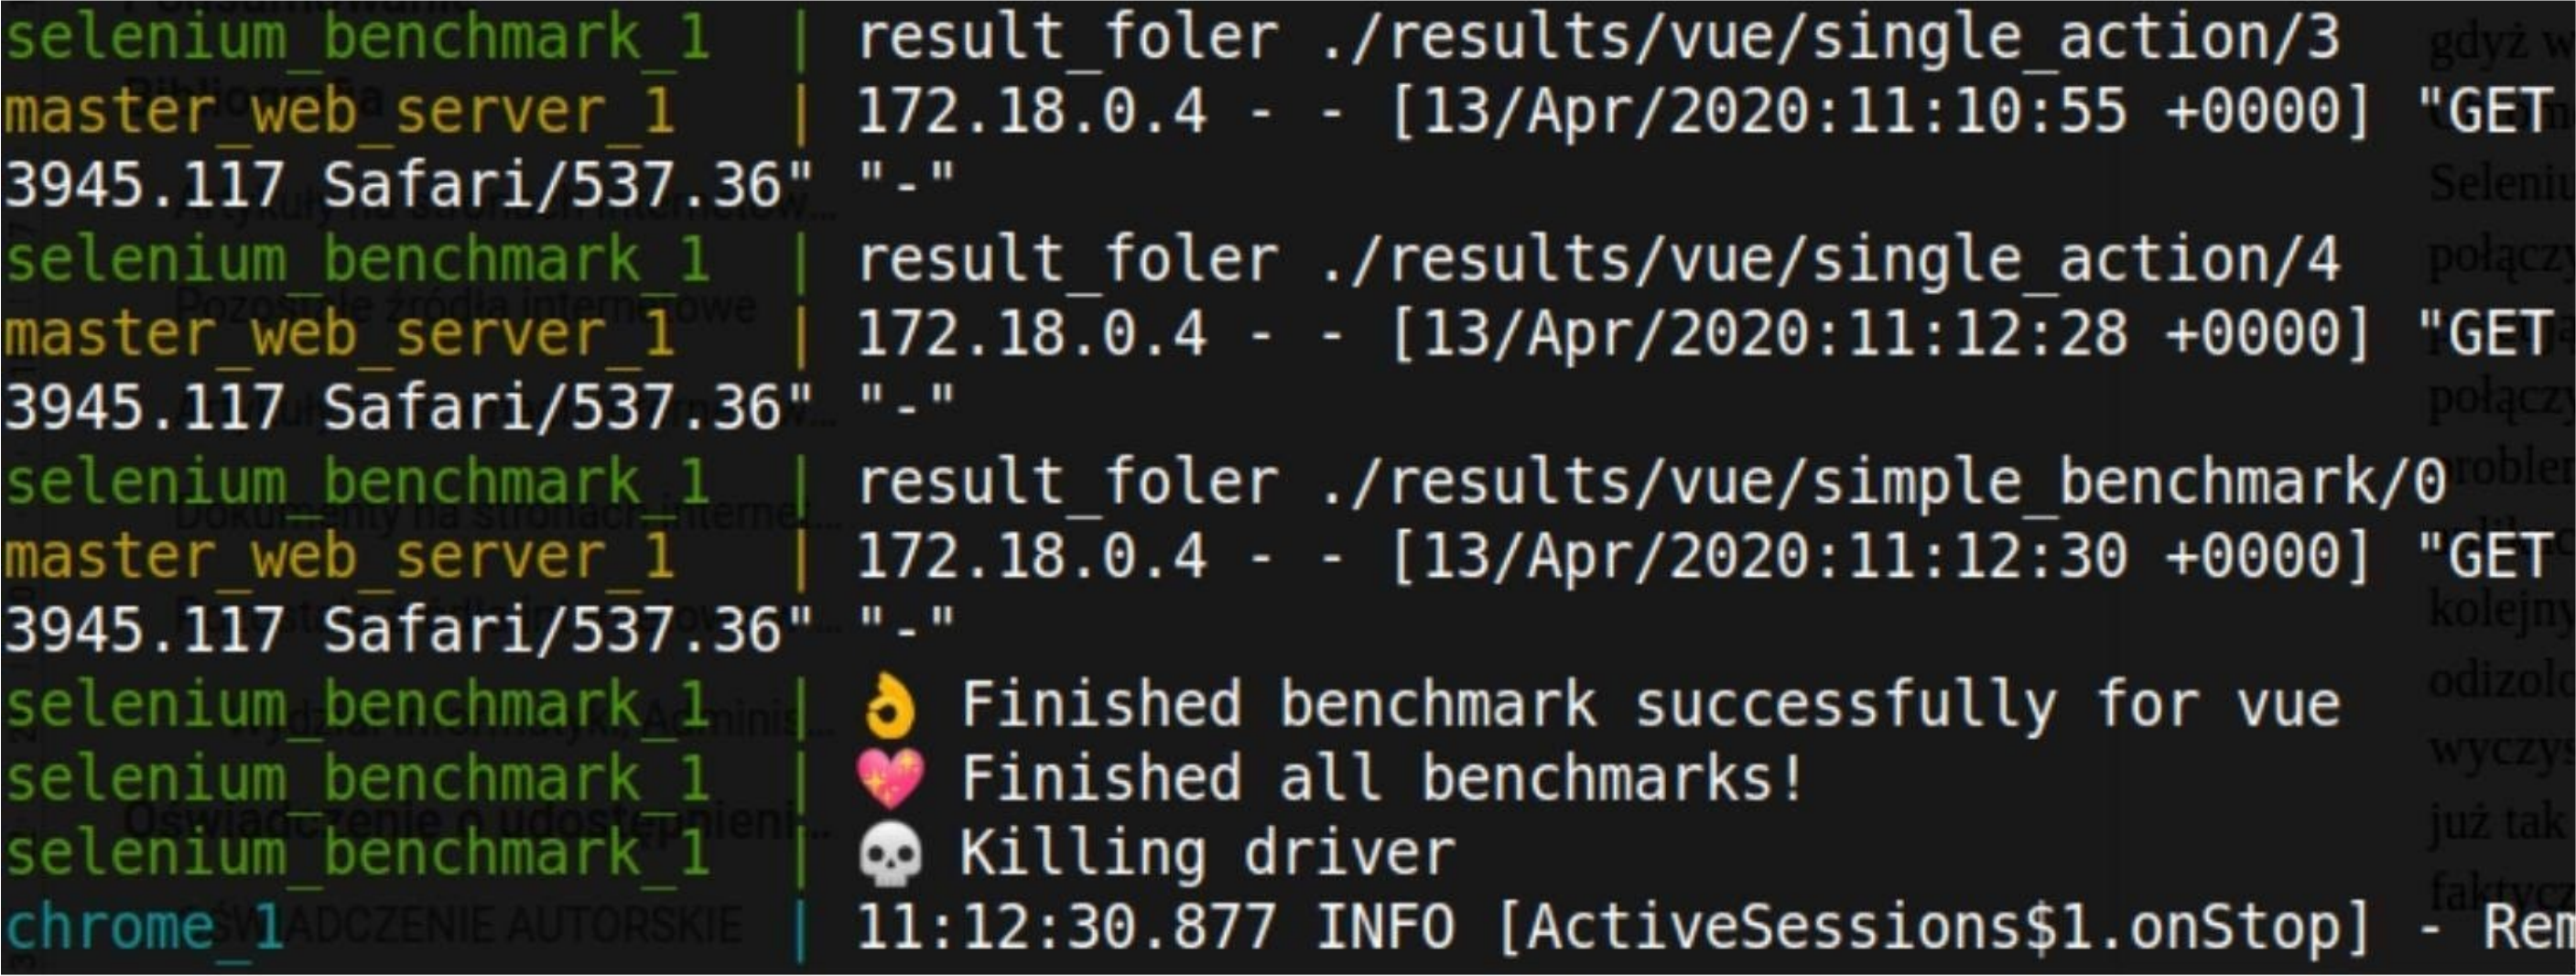
\includegraphics[width=\textwidth]{rysunek_27.png}
    \caption{Grafika przedstawia skrypt zakańczający badanie po zapisaniu zebranych danych na dysk - widzimy, że ważnym elementem jest zamknięcie połączenia do Selenium}
    \label{fig:rysunek_27}
\end{figure}

\subsection{Moduł analizy}

W module tym, zajmiemy się przygotowaniem zebranych danych i skondensowanym ich do postaci pojedynczego pliku JSON zawierającego istotne dla nas informacje.
Skrypt ten jest napisany w sposób generyczny, tak więc dla każdego nowego rodzaju testu powinniśmy przygotować nowy skrypt parsujący.
Podstawowa struktura pliku jest jednak ujednolicona i pozwala nam na generyczne procesowanie pliku. Struktura danych przedstawiona została na grafice \ref{fig:rysunek_28}:

\begin{figure}[htbp]
    \centering
    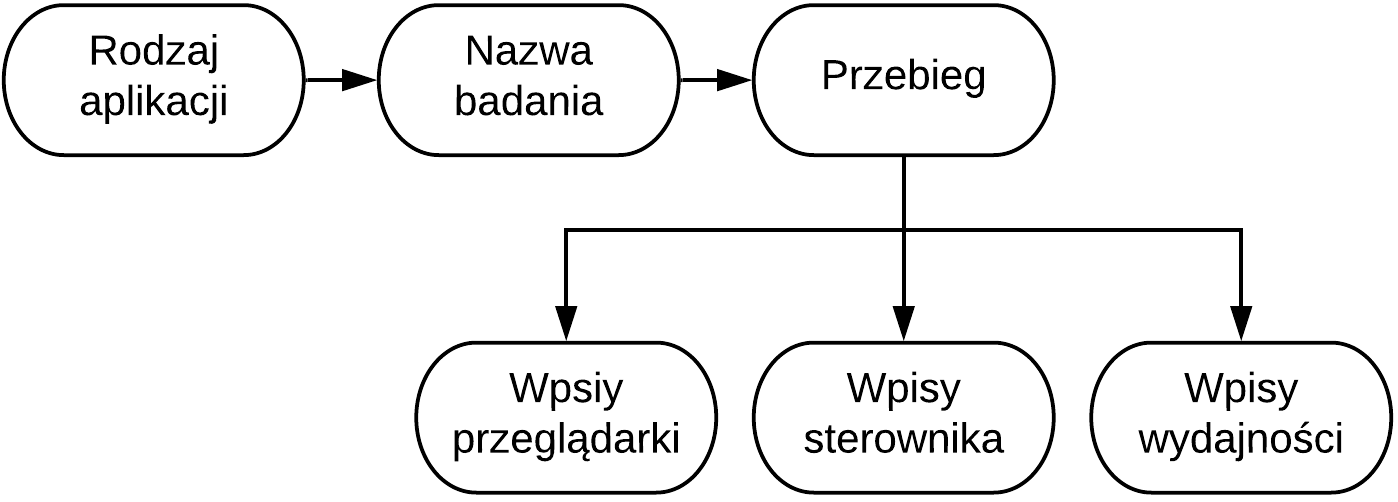
\includegraphics[width=8cm]{rysunek_28.png}
    \caption{Ilustracja struktury wyniku badania na które zostanie poddane dalszej obróbce}
    \label{fig:rysunek_28}
\end{figure}

Dla każdego z dostępnych wpisów, przygotowano po jednej funkcji pozwalającej na ekstrakcję wpisów.
Do celów badania, jedynie wpisy przeglądarki zawierały istotne dane (rysunek \ref{fig:rysunek_29}).
Wynikiem całego skryptu jest pojedyńczy plik index.json zawierający taki sam podział na aplikacje, badania i przebiegi.
Atomowym wpisem dla każdego badania jest pomiar. Pomiar zawiera w sobie nazwę akcji jaka została wykonana oraz zmierzoną wartość.

\begin{figure}[htbp]
    \centering
    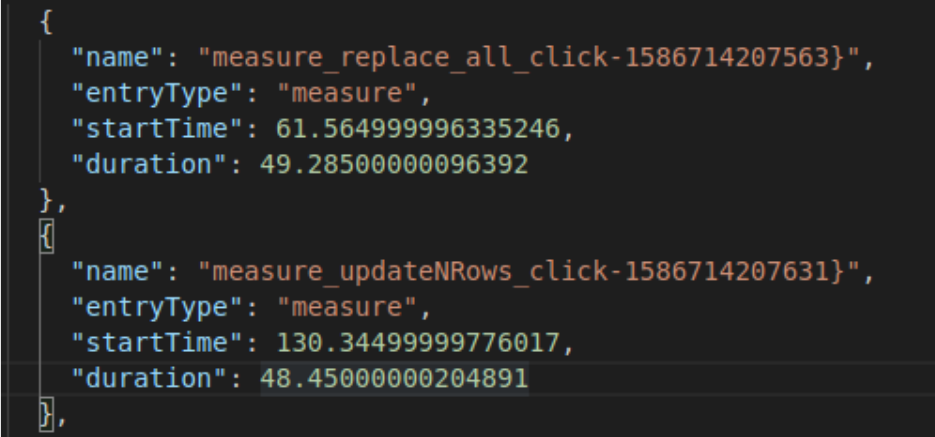
\includegraphics[width=\textwidth]{rysunek_29.png}
    \caption{Grafika przedstawiająca wpis zebranego pomiaru}
    \label{fig:rysunek_29}
\end{figure}

\clearpage
\section{Analiza wyników}

Finalny zestaw badań jakie wykonano objęły następujące parametry:
\begin{itemize}
    \item Test wykonano dla 20 powtórzeń dla każdej aplikacji, czyli łącznie 60 powtórzeń
    \item Każda akcja została powtórzona 100 razy w ramach jednego testu, czyli 2000 razy w ramach pojedynczego badania
    \item Łączna liczba punktów pomiarowych wyniosła 42000 pomiarów
    \item Na potrzeby pracy przyjęto błąd pomiarowy równy $\pm$ 1 milisekunda
\end{itemize}

\subsection{Czas załadowania aplikacji}

Pierwsze badanie polega na zmierzeniu czasu potrzebnego do rozpoczęcia malowania strony. Oczekujemy tutaj na zdarzenie first paint \cite{mdn-first-paint}.
Wyniki zaprezentowano na rysunku \ref{fig:rysunek_30}.

\begin{figure}[htbp]
    \centering
    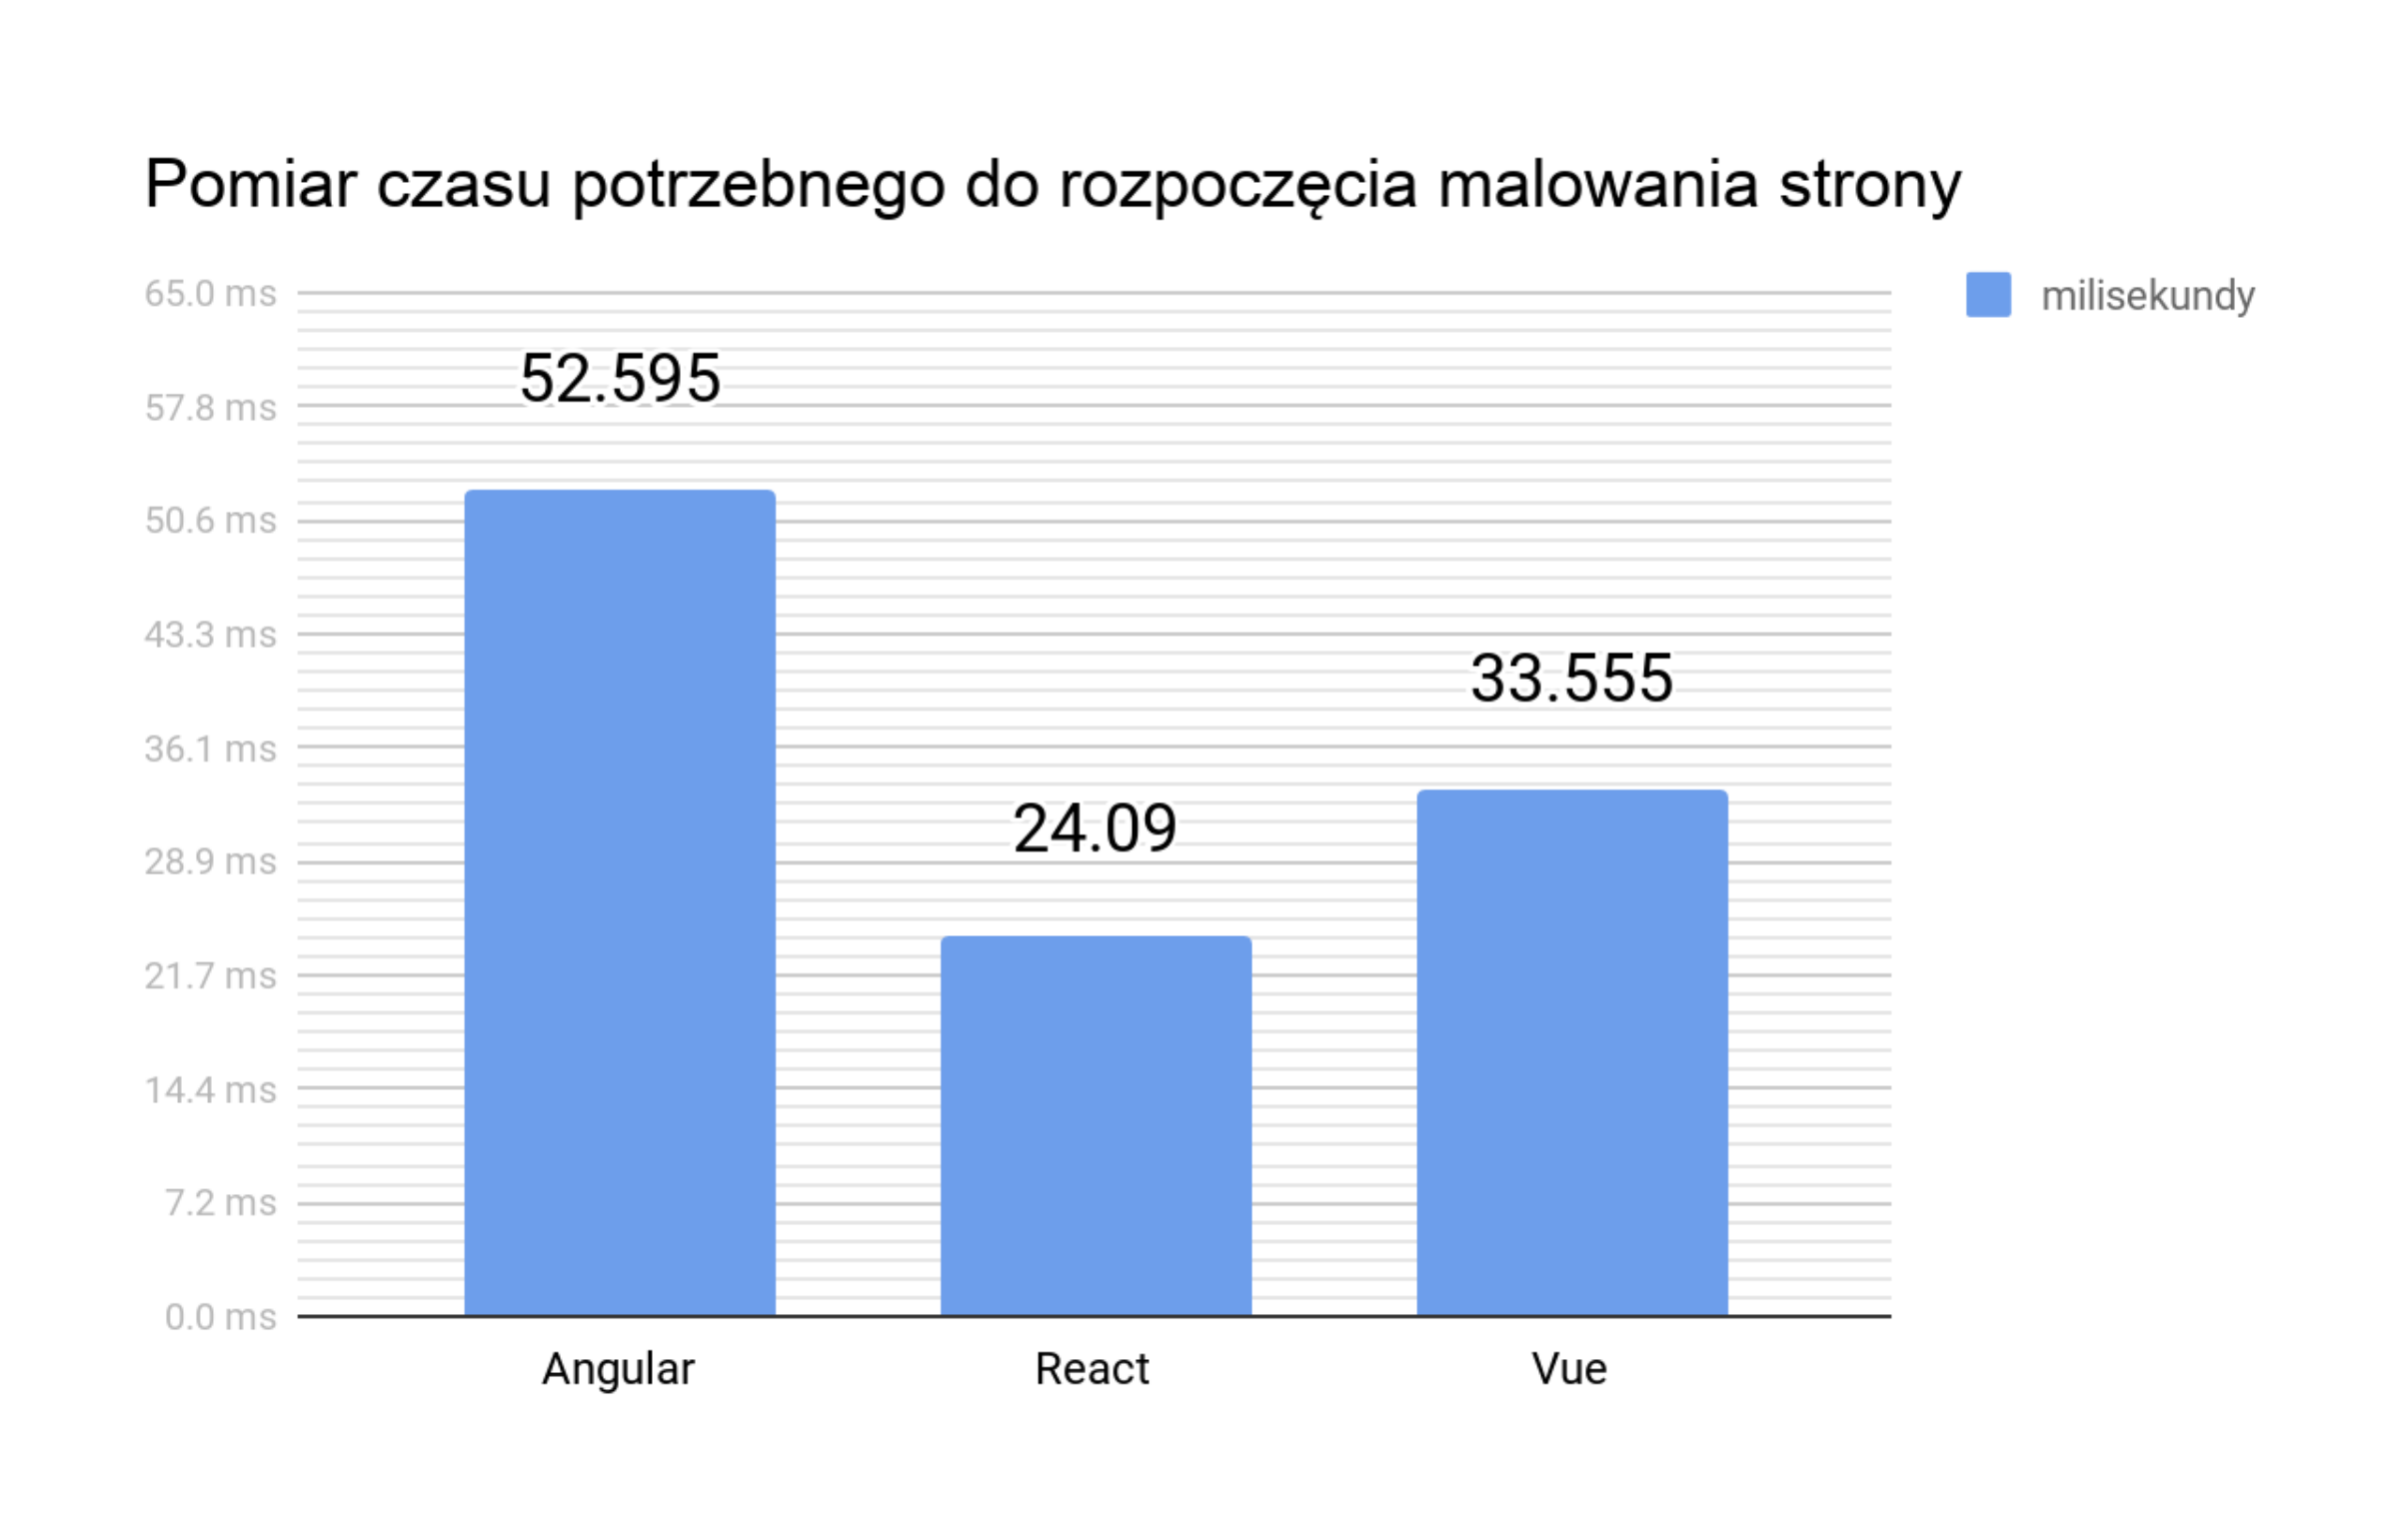
\includegraphics[width=\textwidth]{rysunek_30.png}
    \caption{Diagram kolumnowy ukazujący wynik badania czasu potrzebnego do rozpoczęcia malowania strony}
    \label{fig:rysunek_30}
\end{figure}

Każdy pomiar miał miejsce w czasie odświeżenia strony.
Podane wartości są średnimi wartościami z 20 przeładowań.
Widzimy ogromną różnicę w otrzymanych wynikach. React jest o 9.465 milisekundy szybszy, czyli o 39.290\% szybszy od Vue.
Vue jest także o 19.04 milisekundy szybsze od Angulara co stanowi 56.743\% lepszy wynik.

Główny wpływ na otrzymane wyniki będą mieć waga narzędzia oraz ilość kodu który musi być pobrany oraz uruchomiony zanim narzędzie zacznie renderować wymaganą treść.
Dodatkowe informacje możemy wyłuskać patrząc na ilość bajtów pobranych przez przeglądarkę co ukazano na rysunku \ref{fig:rysunek_31} - Angular2, rysunek \ref{fig:rysunek_32} - React oraz rysunek \ref{fig:rysunek_33} - Vue.

\begin{figure}[htbp]
    \centering
    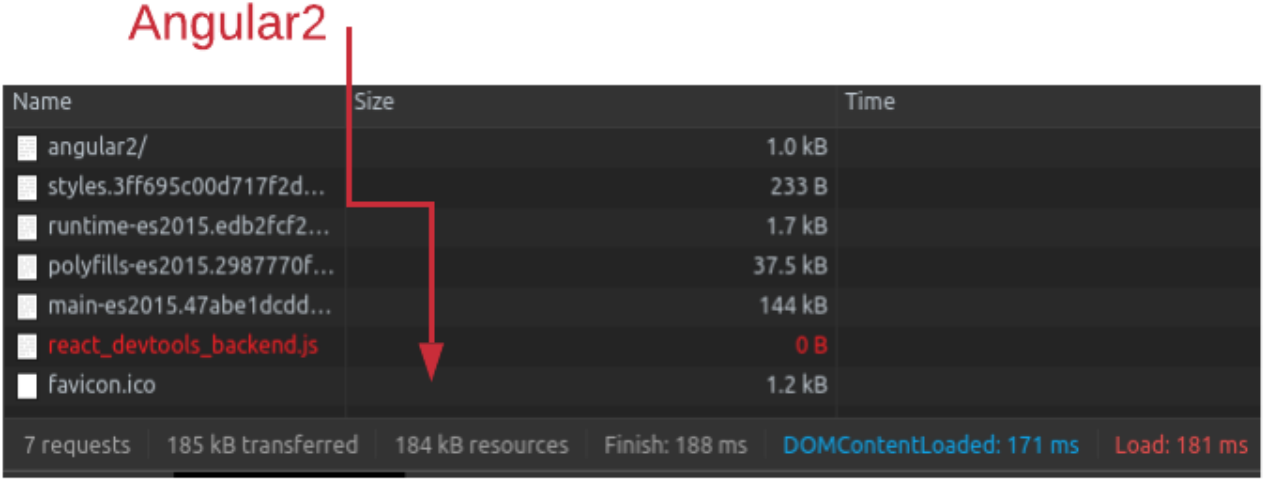
\includegraphics[width=\textwidth]{rysunek_31.png}
    \caption{Grafika ukazująca rozmiar plików zasobów dla aplikacji Angular2}
    \label{fig:rysunek_31}
\end{figure}

\begin{figure}[htbp]
    \centering
    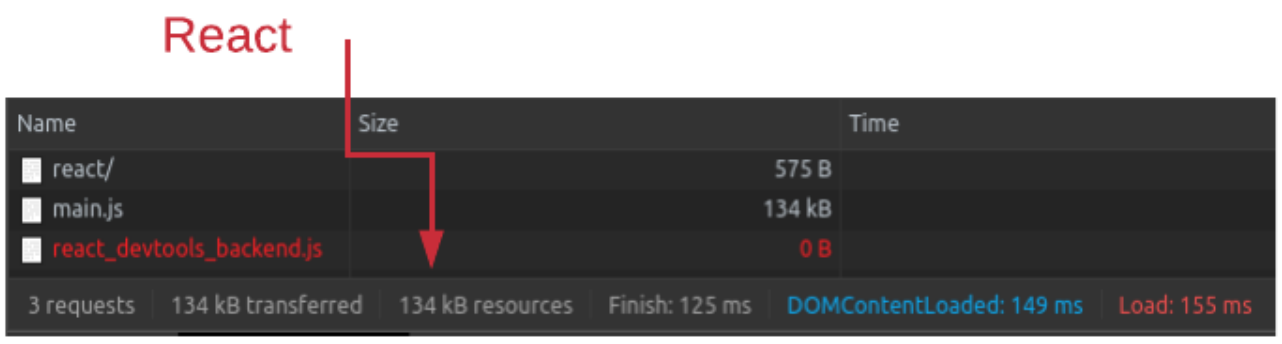
\includegraphics[width=\textwidth]{rysunek_32.png}
    \caption{Grafika ukazująca rozmiar plików zasobów dla aplikacji React}
    \label{fig:rysunek_32}
\end{figure}

\begin{figure}[htbp]
    \centering
    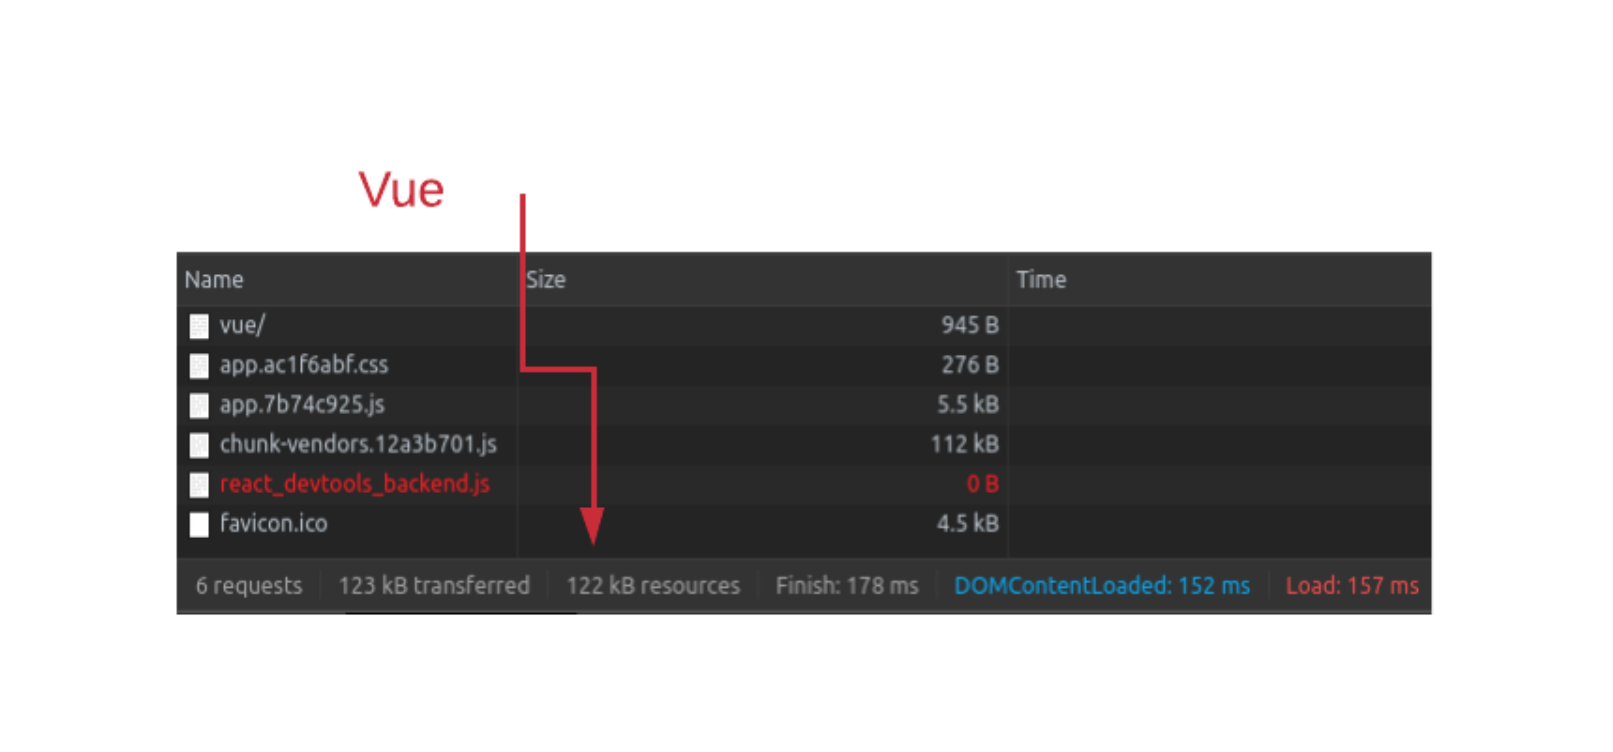
\includegraphics[width=\textwidth]{rysunek_33.png}
    \caption{Grafika ukazująca rozmiar plików zasobów dla aplikacji Vue}
    \label{fig:rysunek_33}
\end{figure}

Wniosek nasuwa się następujący. React który potrzebuje 134 kB danych potrzebuje 24.09 milisekund na wyrenderowanie pierwszego piksela.
Vue który pobiera 122 kB czyli o 8.955\% mniej danych, ładuje się w czasie 33.555 milisekund.
Wskazuje to jednoznacznie, że kod Reacta pomimo większej wagi, wykonuje mniej operacji przed pierwszym renderowaniem.
Na ostatnim miejscu w tym badaniu znajduje się Angular2 który potrzebuje 185 kB oraz 52.595 milisekund na załadowanie pierwszego piksela.

\clearpage
\subsection{Dodanie 1000 wierszy na początku listy}

W badaniu tym do istniejącej listy 1000 elementów dodajemy kolejne 1000 elementów na początek listy.
Akcję tą powtarzamy 100 krotnie, czyli zaczynając od 1000 elementów aż do 101 000 kończąc.
Problem badawczy tego zadania opisano w rozdziale Projekt testu wydajności.
Wyniki badania zobrazowano na rysunku \ref{fig:rysunek_34}.

\begin{figure}[htbp]
    \centering
    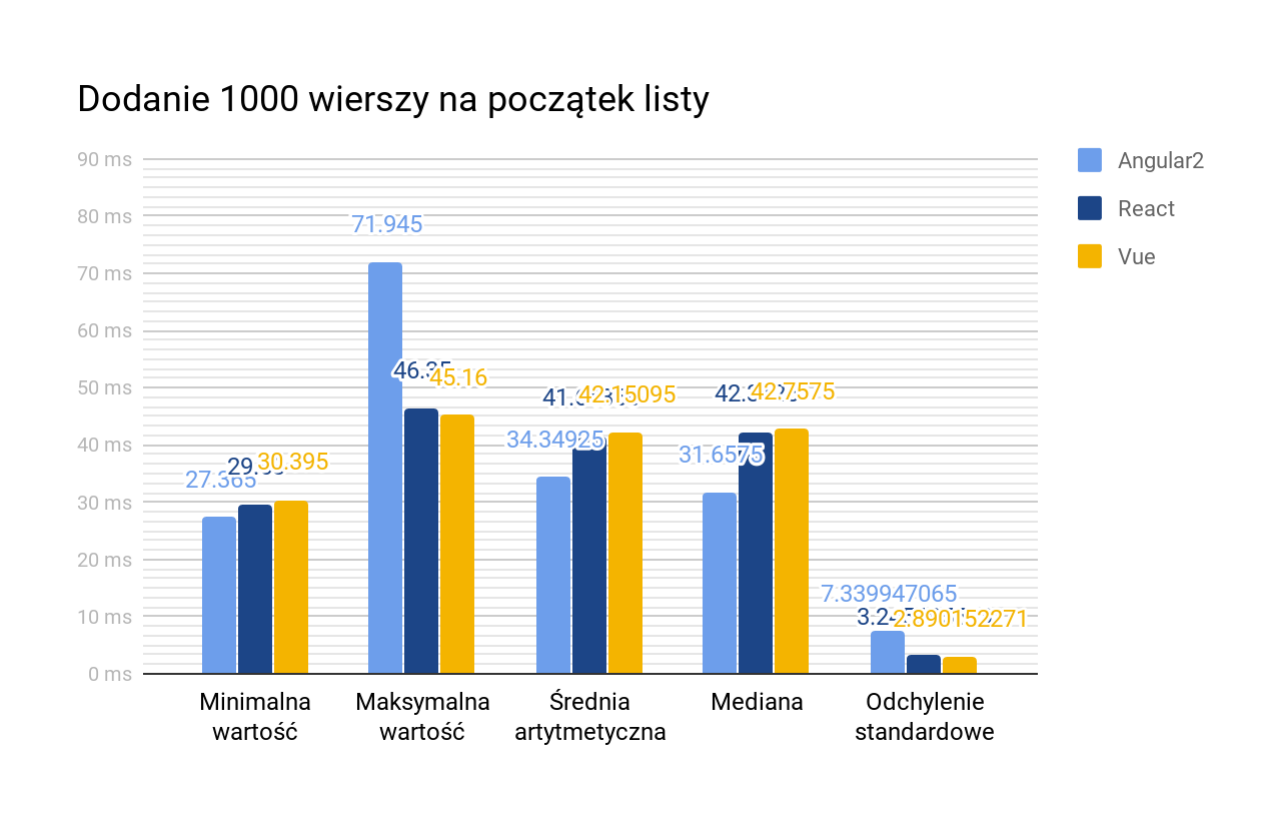
\includegraphics[width=\textwidth]{rysunek_34.png}
    \caption{Diagram kolumnowy obrazujący wynik badania pomiaru czasu dodania 1000 elementów na początek listy}
    \label{fig:rysunek_34}
\end{figure}

Z wykresu wartości, możemy odczytać, iż wartości brzegowe Angular2 wyznaczają dolną oraz górną granicę otrzymanych wartości czasu.
Także odchylenie standardowe jest ponad dwukrotnie wyższe niż kolejny po nim React.
Jednak średnia i mediana wskazują, że w uśrednionym przypadku, dopisywanie nowych elementów do listy jest najszybsze w frameworku Angular2.
React oraz Vue w przypadku uśrednionym, plasują się na drugiej pozycji, gdyż ich wartości mieszczą się w wartości błędu pomiaru.
Najmniejsze rozproszenie wyników prezentuje Vue, którego średnia i mediana są bardzo zbliżone,
a odchylenie standardowe najniższe spośród badanych narzędzi, co świadczy o stabilności rozwiązania.

\clearpage
\subsection{Dodanie 1000 wierszy na końcu listy}

Dopisywanie elementów do końca listy jest mało obciążającym zadaniem dla naszych narzędzi. Nie musimy przesuwać żadnych elementów, jedynie wyrenderować nowo dodane.
Oczekujemy, iż wyniki (rysunek \ref{fig:rysunek_35}) będą miały małe odchylenie standardowe (gdyż ilość poprzednich elementów nie powinna mieć wpływu na dodanie nowych).

\begin{figure}[htbp]
    \centering
    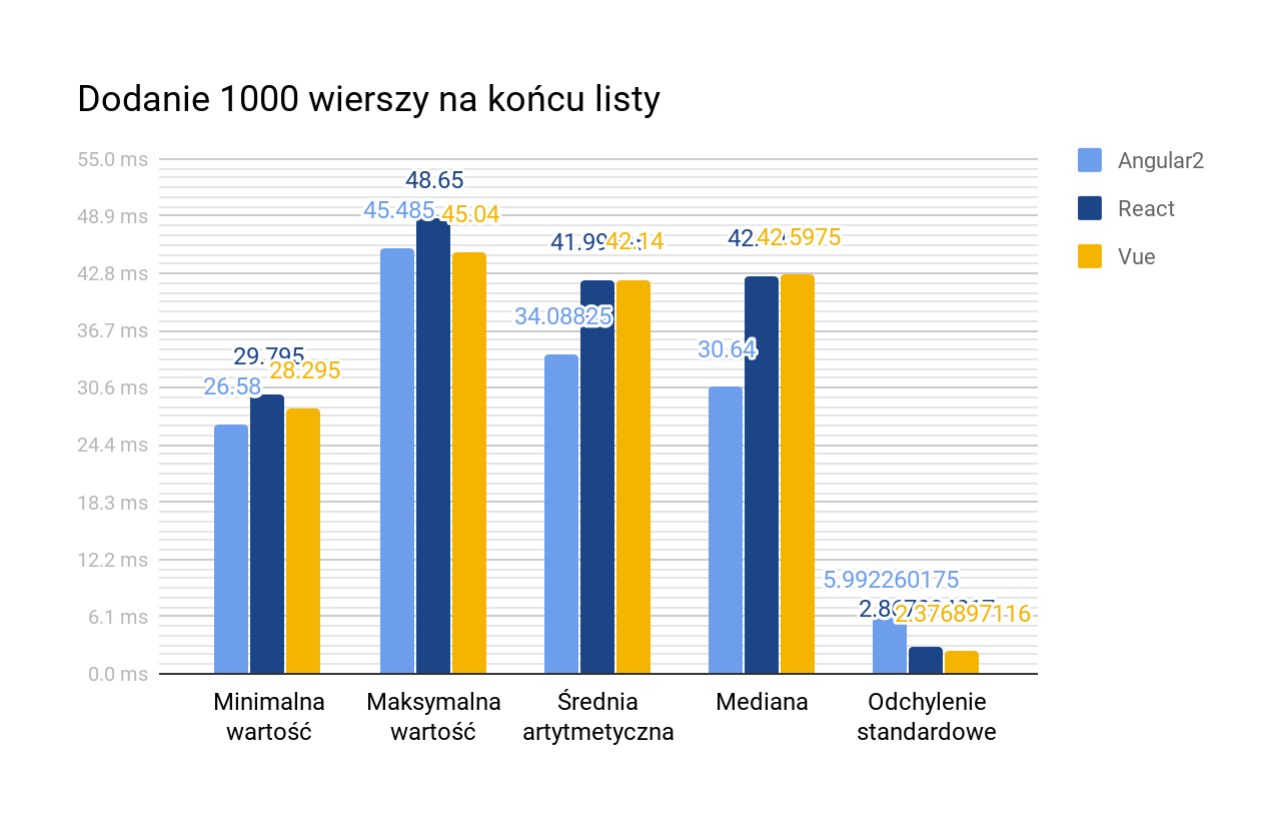
\includegraphics[width=\textwidth]{rysunek_35.png}
    \caption{Diagram kolumnowy obrazujący wynik badania pomiaru czasu dodania 1000 elementów na koniec listy}
    \label{fig:rysunek_35}
\end{figure}

Pierwszym, co można zauważyć, jest fakt iż dla przypadku minimalnej wartości oraz maksymalnej wartości, wyniki pomiędzy narzędziami są zbliżone.
Jednak warto zaznaczyć, iż React jest najwolniejszy w skrajnych przypadkach.
W uśrednionym przypadku, Angular2 jest najszybszym narzędziem bijąc React oraz Vue o 8 milisekund w przypadku średniej a w przypadku mediany o aż 12 milisekund.
Jednak warto zaznaczyć, iż odchylenie standardowe tego badania wskazuje, że Angular2 jest najmniej przewidywalnym z całej trójki.
Ciekawą sytuację natomiast możemy zaobserwować dla wyników średniej oraz mediany pomiędzy React oraz Vue.
Wyniki są bardzo zbliżone, jednak odchylenie standardowe wskazuje, że to Vue jest stabilniejszym rozwiązaniem.

\clearpage
\subsection{Zamiana wszystkich wierszy na liście}

Badanie to wskazuje, jak szybko jesteśmy w stanie przerenderować listę 1000 elementów. Wyniki ukazano na rysunku \ref{fig:rysunek_36}.

\begin{figure}[htbp]
    \centering
    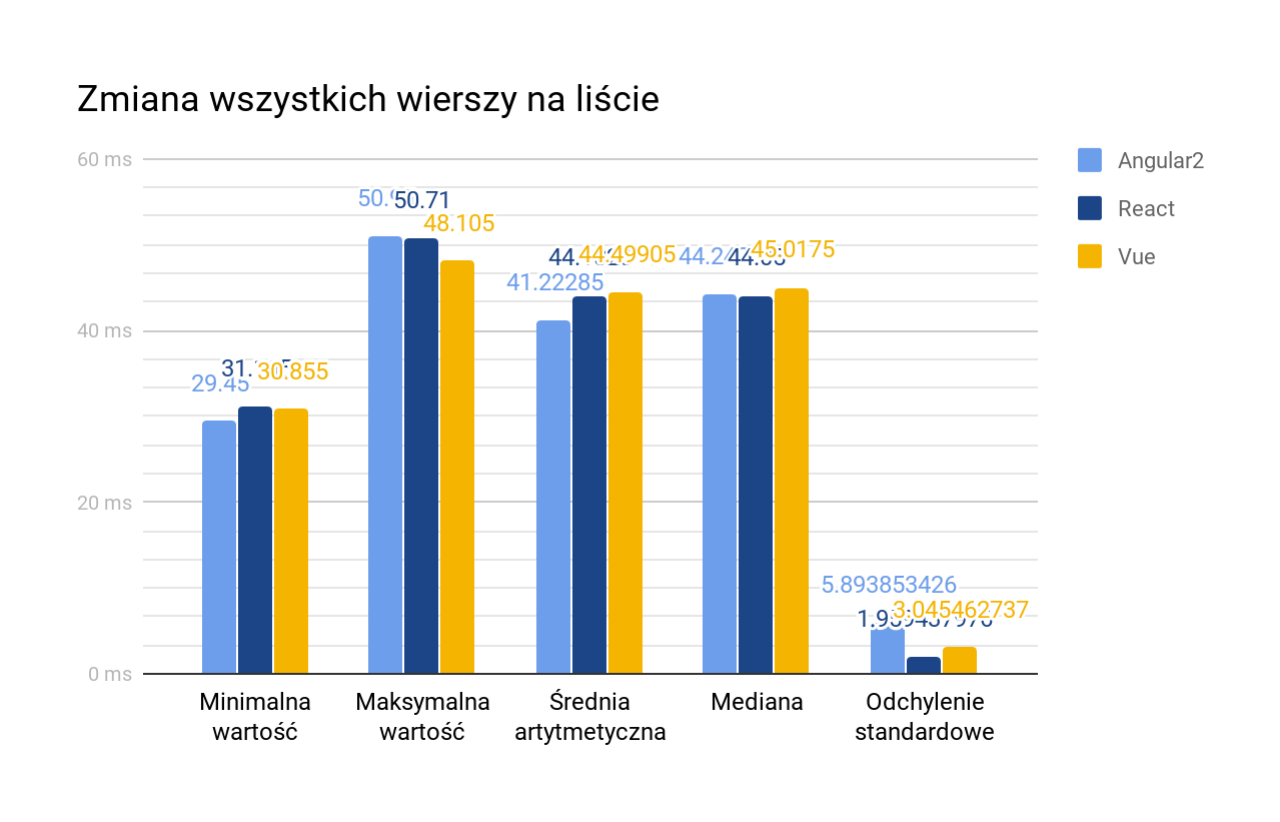
\includegraphics[width=\textwidth]{rysunek_36.png}
    \caption{Diagram kolumnowy obrazujący wynik badania pomiaru czasu zmiany wszystkich wartości listy dla 1000 elementów}
    \label{fig:rysunek_36}
\end{figure}

Minimalna wartość jest bardzo zbliżona dla każdego z badanych narzędzi. Maksymalna wartość wskazuje nieznaczną przewagę około 2 milisekund na korzyść Vue.
Średnia arytmetyczna wskazuje nam, iż Angular2 jest najszybszym narzędziem, jednak odchylenie standardowe wskazuje, iż jest także najbardziej niestabilnym.
W tym badaniu React udało się uzyskać odchylenie poniżej 2 milisekund, co jest wynikiem bardzo dobrym.

\clearpage
\subsection{Aktualizacja 500 wierszy}
W badaniu tym, aktualizujemy tylko połowę wyrenderowanych wierszy. Wyniki ukazano na rysunku \ref{fig:rysunek_37}.
\begin{figure}[htbp]
    \centering
    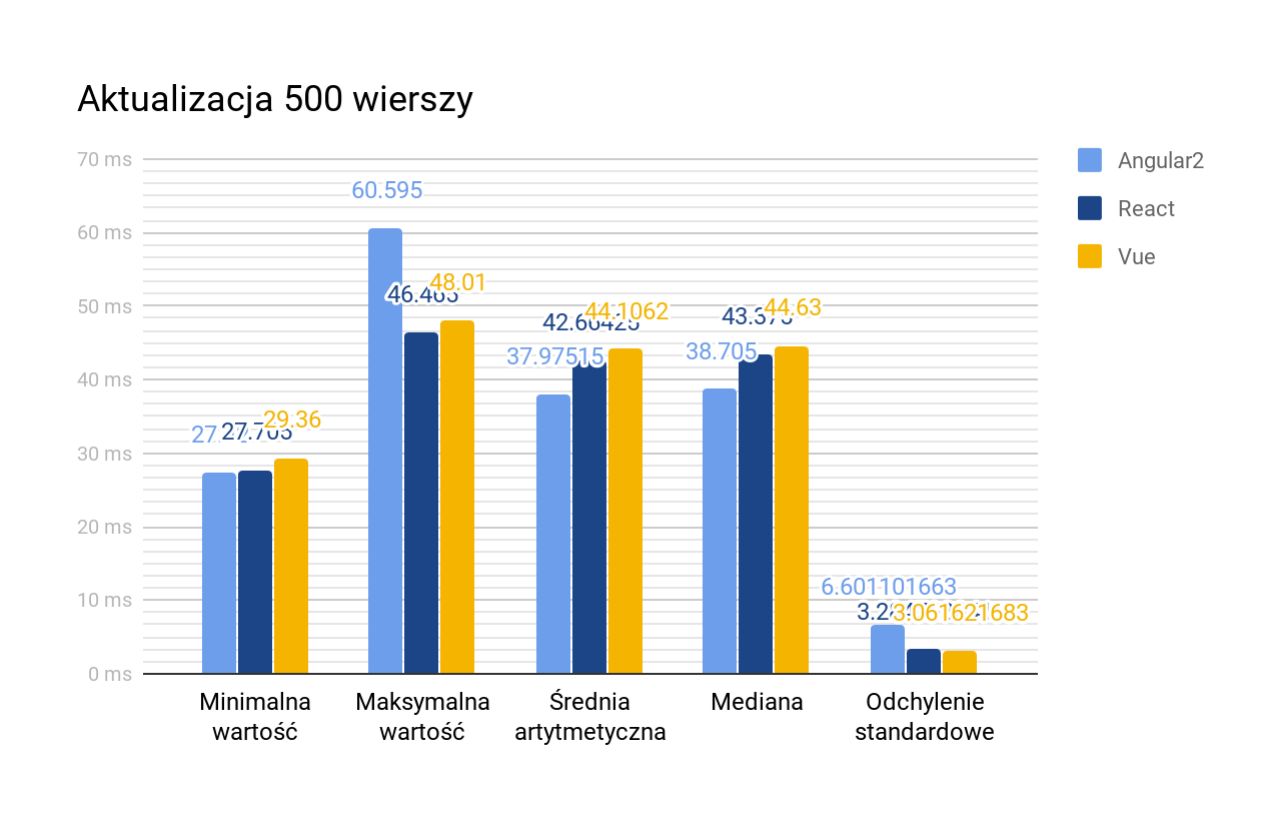
\includegraphics[width=\textwidth]{rysunek_37.png}
    \caption{Diagram kolumnowy obrazujący wynik badania pomiaru czasu zmiany wartości dla 500 elementów listy}
    \label{fig:rysunek_37}
\end{figure}
Wartości minimalne są bardzo zbliżone dla Reacta oraz Angular2. Vue odbiega tylko nieznacznie mniej niż 2 milisekundy.
W przypadku wartości maksymalnych, Angular2 znacząco odbiega od reszty narzędzie wykazuje różnicę 12 milisekund do kolejnego na liście Vue.
W uśrednionym przypadku, widzimy zgodność średniej arytmetycznej i mediany, które wskazują, iż Angular2 jest najszybszym narzędziem.
Ponownie już odchylenie standardowe wskazuje iż jest także najmniej stabilnym czasowo narzędziem.

\clearpage
\subsection{Zamiana miejscami dwóch wierszy}

Zamiana miejscami dwóch wierszy jest najmniej wymagającym badania z całej pracy. Z tego powodu oczekujemy niskich wartości odchylenia standardowego. Wyniki ukazano na rysunku \ref{fig:rysunek_38}.

\begin{figure}[htbp]
    \centering
    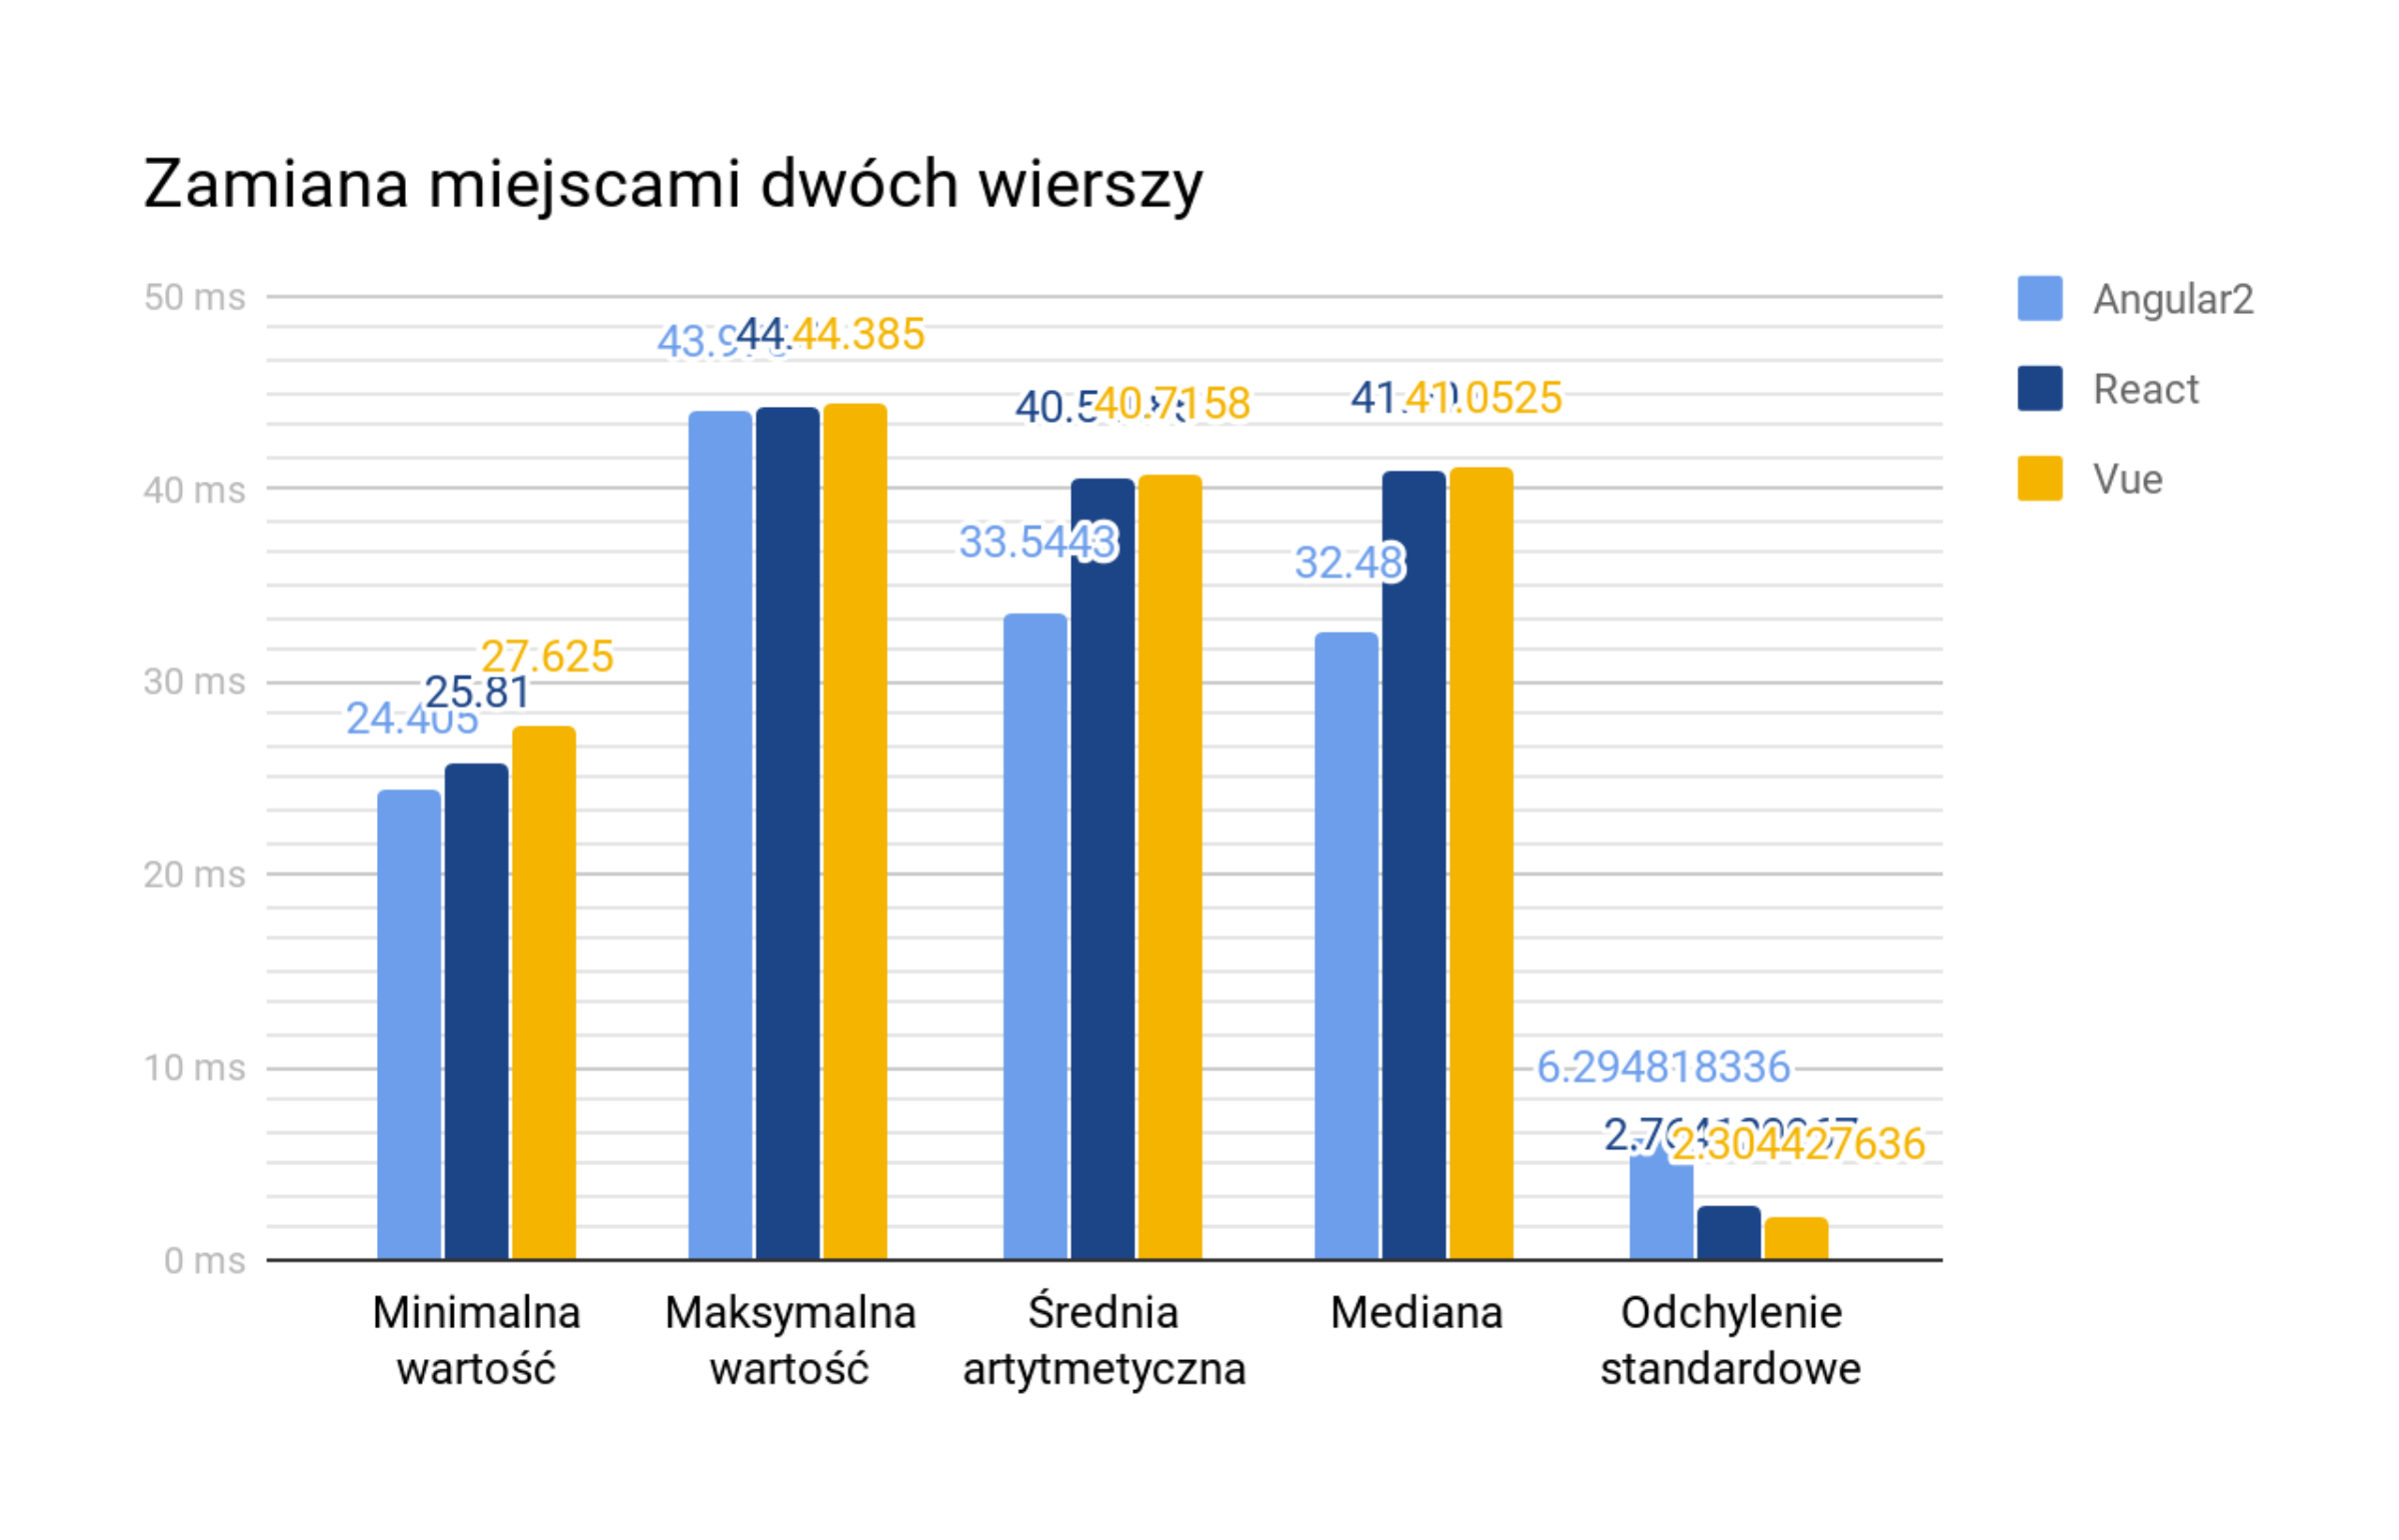
\includegraphics[width=\textwidth]{rysunek_38.png}
    \caption{Diagram kolumnowy obrazujący wynik badania pomiaru czasu zamiany miejscami dwóch wartości na liście elementów}
    \label{fig:rysunek_38}
\end{figure}

I tak wartość minimalna wskazuje, iż Angular2 jest najszybszy. Wartości maksymalne są prawie identyczne.
Są one w granicy błędu pomiarowego. Średnia arytmetyczna i mediana zgodnie wskazują, iż Angular2 jest najszybszy w średnim przypadku, znowu z zastrzeżeniem, gdyż odchylenie standardowe wynosi aż 6.3 milisekundy.

\clearpage
\subsection{Usunięcie pojedynczego wiersza}

Badanie to polega na usunięciu pierwszego w kolejności wiersza na początku listy. Powoduje to przesunięcie całej listy o jeden wiersz. Wyniki ukazano na rysunku \ref{fig:rysunek_39}.

\begin{figure}[htbp]
    \centering
    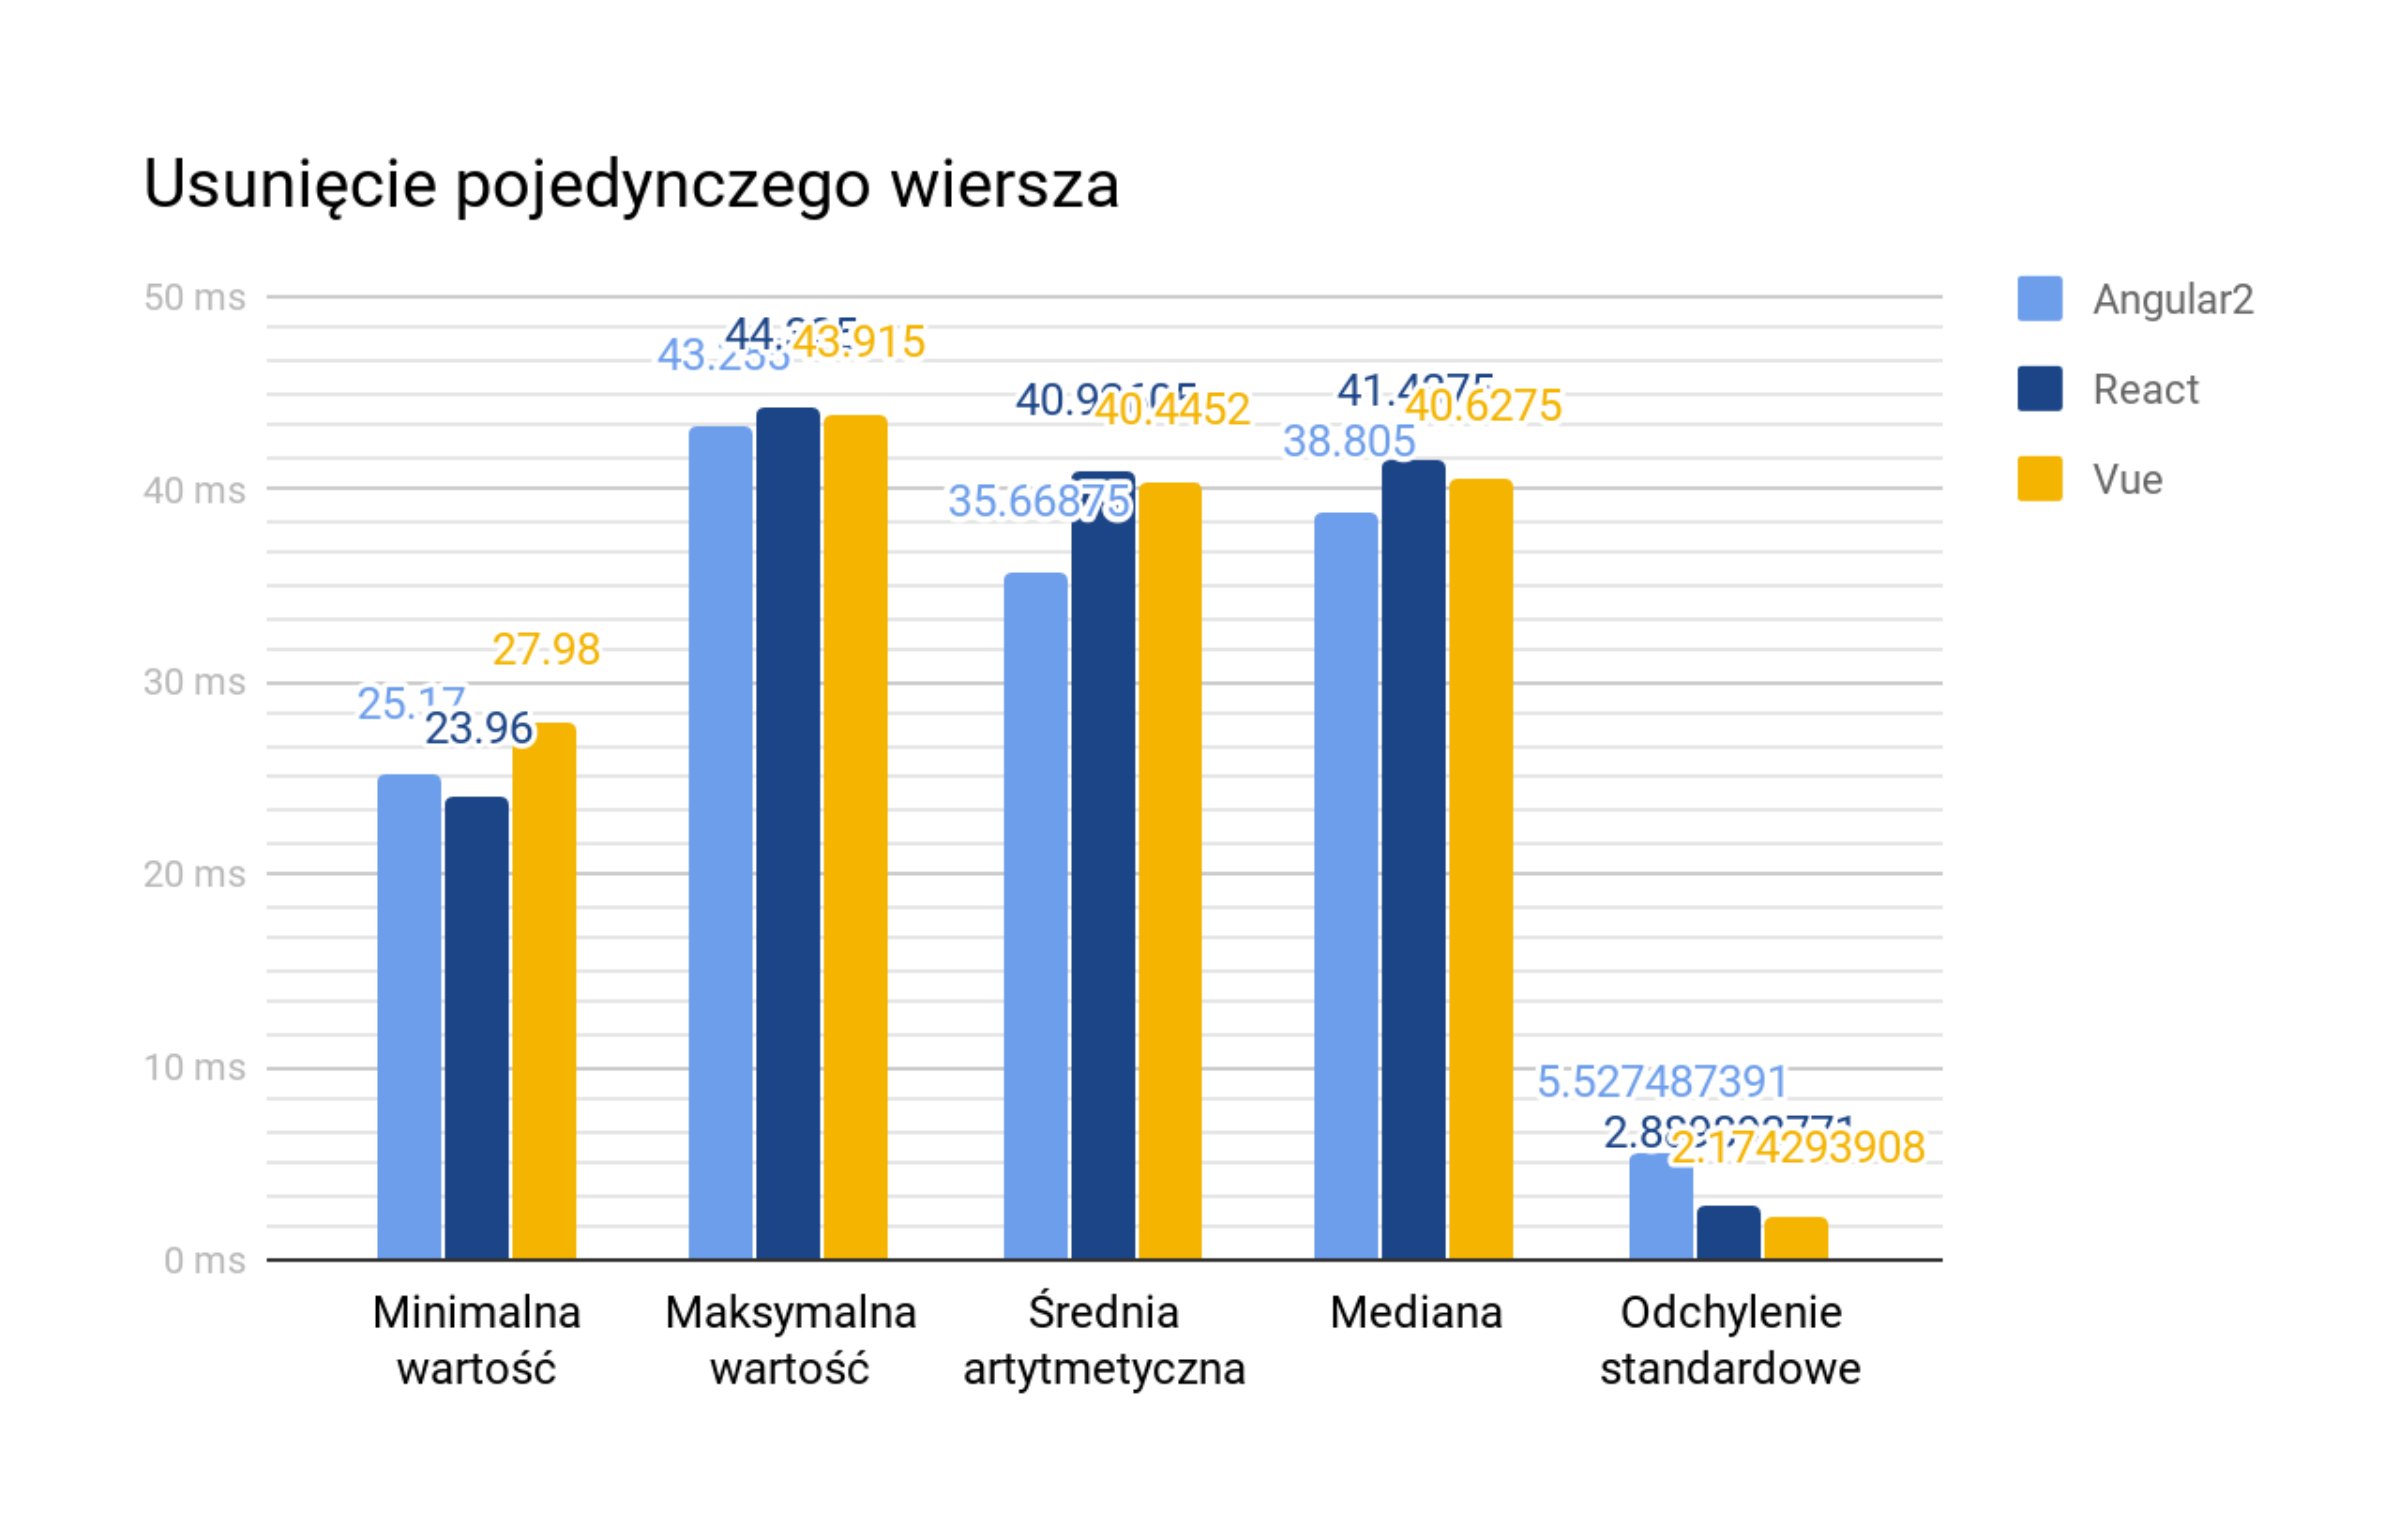
\includegraphics[width=\textwidth]{rysunek_39.png}
    \caption{Diagram kolumnowy obrazujący wynik badania pomiaru czasu usunięcia pojedynczej wartości z listy elementów}
    \label{fig:rysunek_39}
\end{figure}

Po raz pierwszy obserwujemy Reacta jako najszybsze narzędzie w przypadku wartości minimalnej.
Wartości maksymalne mieszczą się w granicy błędu pomiarowego dla każdego z badanych narzędzi. Średnia arytmetyczna i mediana ponownie wskazują na dominację Angulara 2.
Jednak ponownie odchylenie standardowe wskazuje na znaczące wahania wartości wokół średniej wartości dla Angular2.
Vue oraz React poza wartością minimalną mieszczą się w granicy błędu pomiarowego.

\clearpage
\subsection{Usunięcie wszystkich wierszy}

Ostatnie badanie skupia się na usunięciu wszystkich wierszy. Spowoduje to przerenderowanie całej listy. Wyniki ukazano na rysunku \ref{fig:rysunek_40}. 

\begin{figure}[htbp]
    \centering
    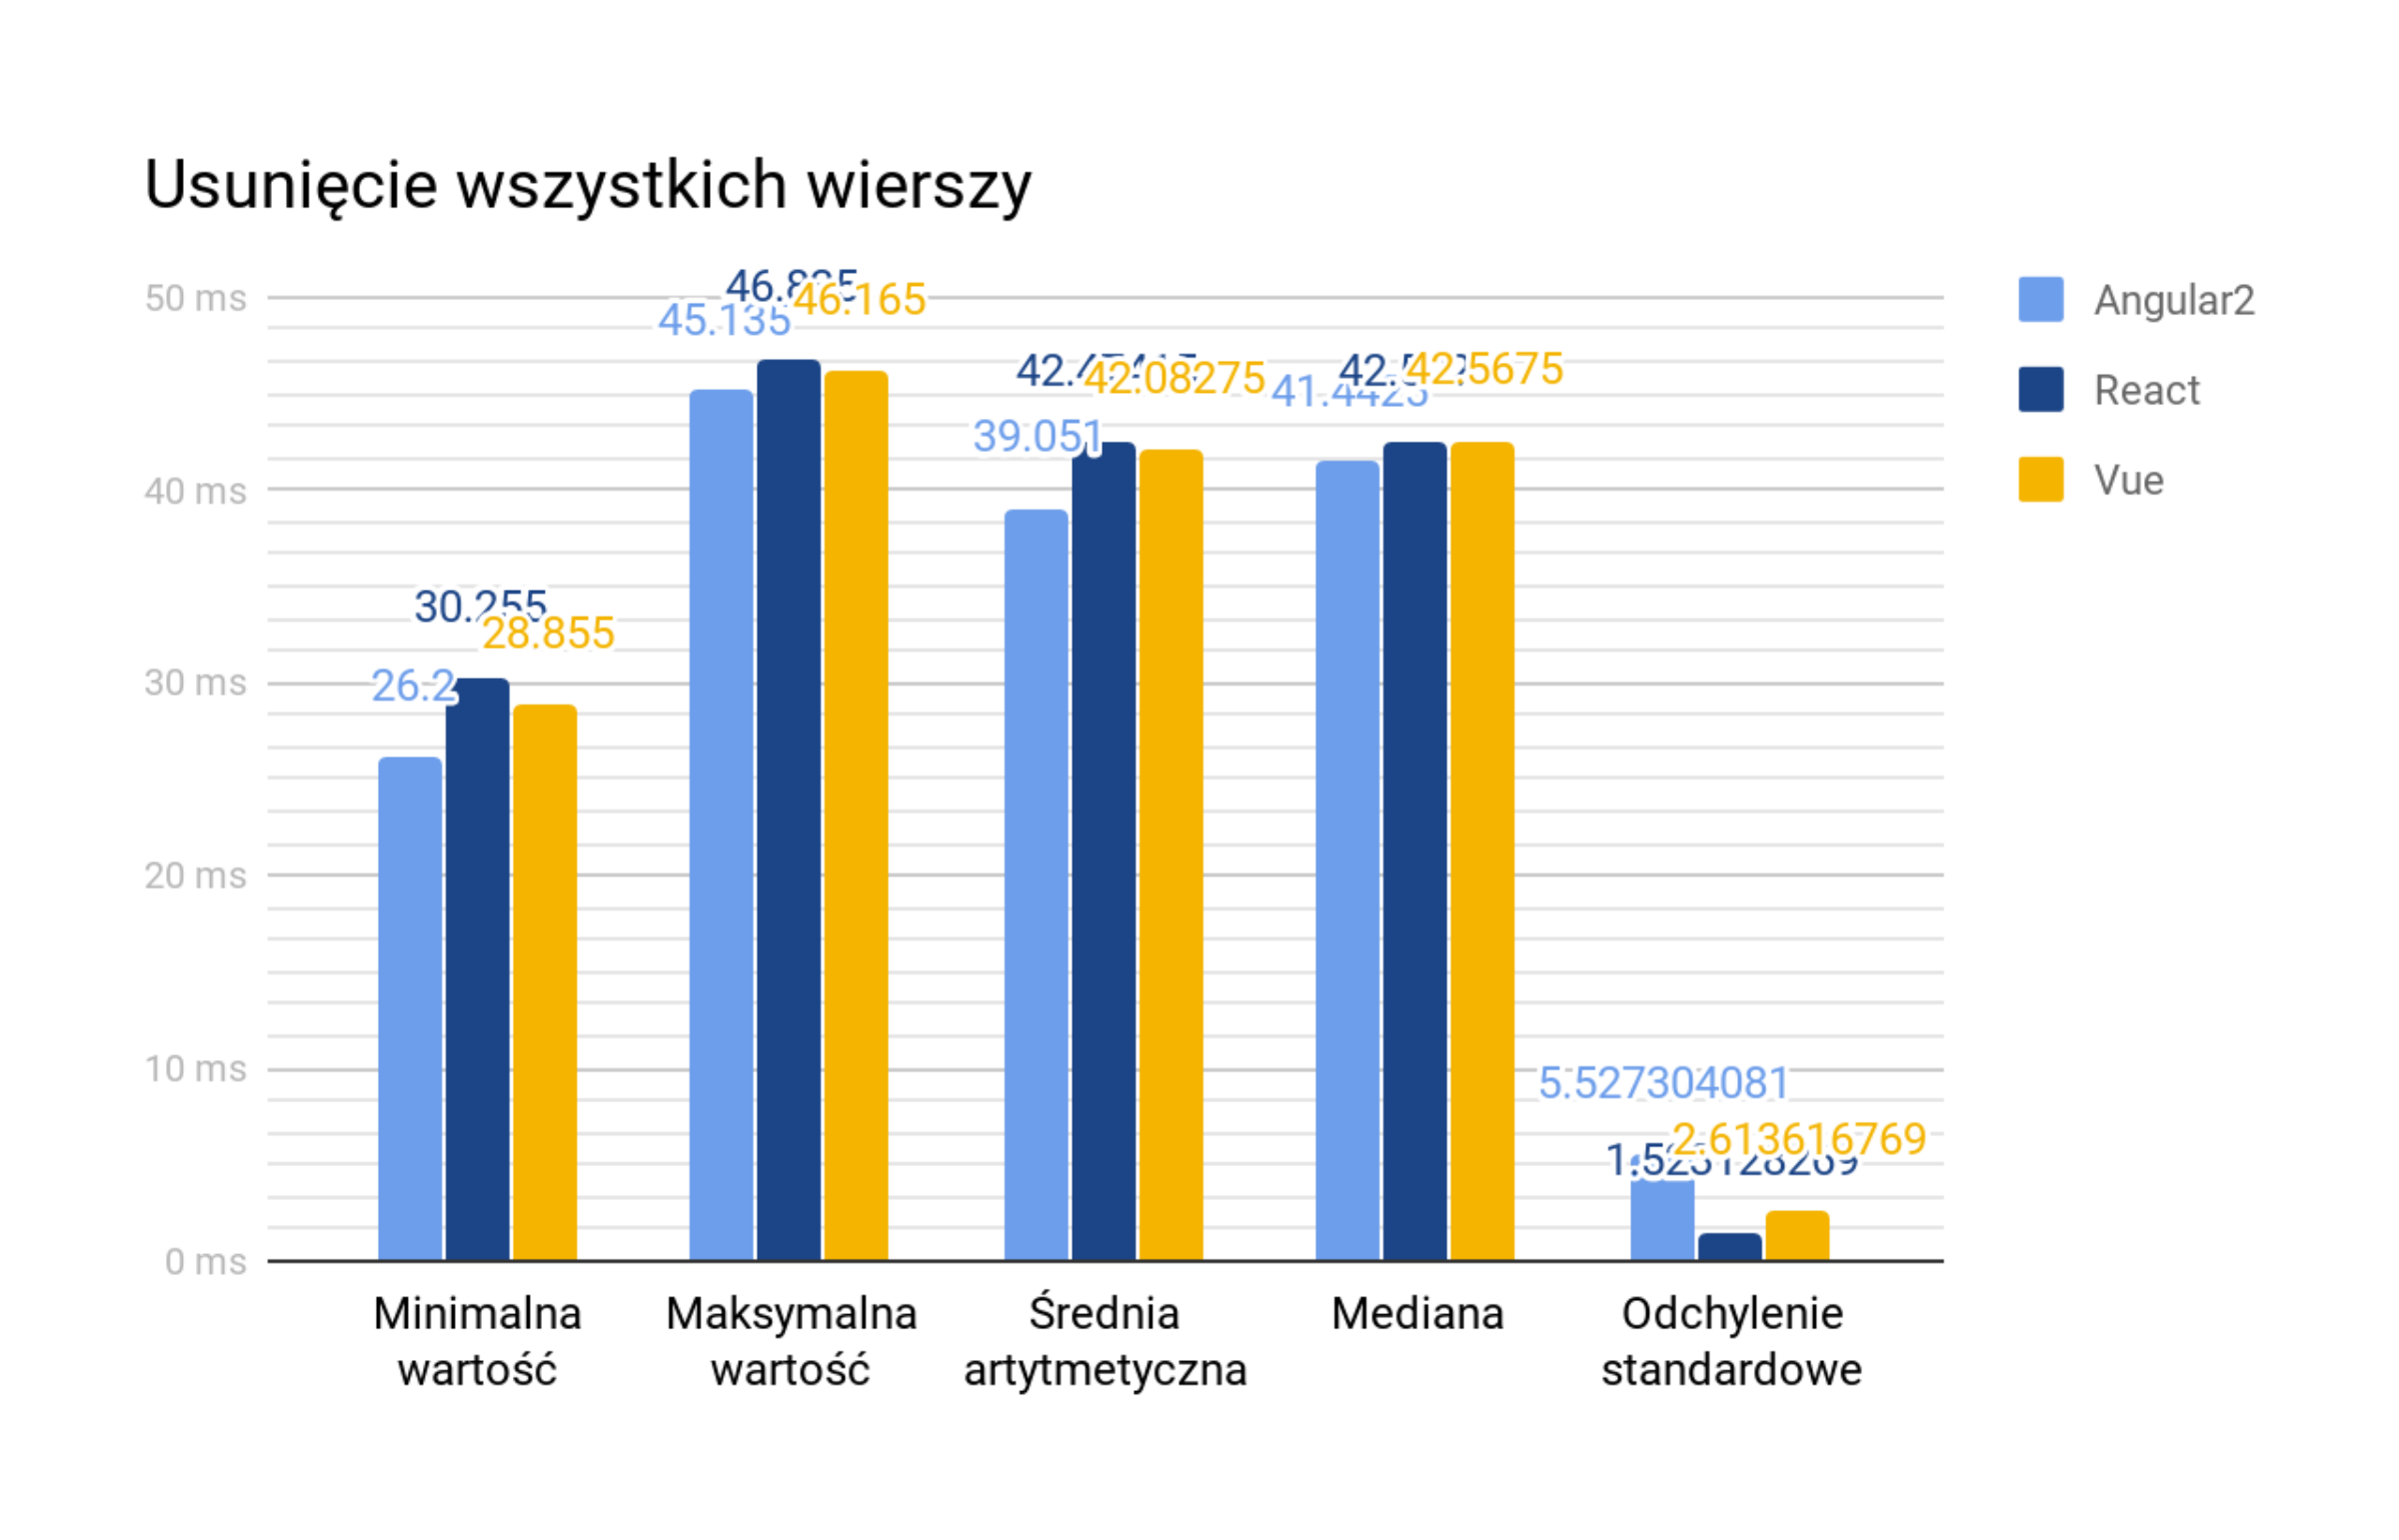
\includegraphics[width=\textwidth]{rysunek_40.png}
    \caption{Diagram kolumnowy obrazujący wynik badania pomiaru czasu usunięcia wszystkich wartości z listy elementów}
    \label{fig:rysunek_40}
\end{figure}

Dla minimalnej wartości Angular2 wykazuje 2 milisekundy przewagi nad kolejnym Vue które z kolei wykazuje około 1.5 milisekundy przewagi nad React.
Wartości maksymalne dla każdego badanego narzędzia mieszczą się w granicy błędu pomiarowego, z delikatnym wskazaniem przewagi dla Angular2.
W średnim przypadku Angular2 jest ponownie najszybszy, lecz odchylenie standardowe wskazuje prawie 5.5 milisekundy zabiegu.
W tym przypadku należy zauważyć, iż React ponownie uzyskał odchylenie standardowe na poziomie 1.5 milisekundy.

%czyści puste strony
\let\cleardoublepage\clearpage